\chapter{Evaluation}\label{ch:evaluation}



\section{Experimental Setup}


    \subsection{Datasets}
    We used two different synthetic datasets to learn our proposed models. We chose to use synthetic datasets due to their completeness, which was essential for our methods. The problem of surface reconstruction with uncertainty quantification from just partial point clouds is already quite challenging, uncertain, and underdetermined. Further lack of information, such as missing regions in ground truth data, would have made it extremely difficult to learn even the surface reconstruction. Uncertainty quantification would be an added challenge. 
    \newline
    
    One of the datasets we used was generated from the popular synthetic 3D point cloud dataset ShapeNet~\cite{ShapeNet}. We follow the same procedure and data split used in~\cite{PCN}. The dataset is created from CAD models of 8 different categories of objects, namely airplane, cabinet, car, chair, lamp, sofa, table, and vessel. There are 30974 models in total, out of which 28794 are used for training. For each model used in training, we have one complete point cloud consisting of 16384 points sampled uniformly on the surfaces defined by meshes and 8 different partial point clouds with different counts of points corresponding to 8 randomly distributed viewpoints. Due to resource constraints, we used 2048 points out of 16384 to represent the complete shapes. We used farthest point sampling to select the points for complete clouds. For partial clouds, we used a maximum of 1024 points for standard learning unless specified otherwise. Out of the remaining 2000 models, 800 were used for validation and 1200 for testing. The validation and test data were equally distributed among different categories, with 100 each for validation and 150 each for testing. 
    \\
    The second dataset we performed our experiments on was used to benchmark different methods for building point cloud completion introduced in~\cite{BuildingPCC}. The dataset consists of around 50000 building models from The Hague and Rotterdam in the Netherlands. It contains 29999 training samples with each complete sample corresponding to 2 viewpoint partial scans, 9998 validation samples, and 10000 testing samples. 


    \subsection{Model Architectures}

        \subsubsection{Point Cloud Completion Networks}
        \textbf{Autoencoder.} 
        For learning the encoding for a given input cloud, we mainly trained an autoencoder (encoder-decoder network), minimizing Earth Mover's Distance for a reconstruction task. We experimented with standard, variational, and vector quantized variational autoencoders. Nevertheless, we mainly perform our experiments with a standard encoder-decoder network. The encoder network E consists of 4 internal fully connected layers with dimensions 64, 128, 128, and 256, respectively. We also added a residual connection between the input and the final internal layer. We chose the latent dimension of the encoding space to be 128 in general unless stated otherwise. Rather than just the coordinates of the point clouds, we use a positional encoding with 6 different encoding functions concatenated with the 3D coordinates as an input to the encoder network. The output of the encoder network is then fed to the decoder network. The decoder network D consists of 2 hidden linear layers, each having 256 nodes. We used leaky rectified linear units as the activation function to allow non-zero gradients for negative values.
        \newline \textbf{Generator.}
        For learning to produce encodings corresponding to complete shapes from the encoding of a partial cloud input, we use a simple generator network. The generator network comprises 2 hidden linear layers with dimensions 256 and 512. For MC dropout or MC DropConnect, the input is just the 128-dimensional encoding of the partial cloud. This is the same for the ensemble of generators, with each generator having the same input. Only for the implicit generative model do we concatenate a noise vector with the encoding before passing it to the generator. We chose the noise dimension to be 32. The hidden layers retain the same structure for all the models except when dropout or DropConnect is applied. We drop weights of nodes with a probability of 0.1 in such methods. Again, we used leaky rectified linear units as the activation function.
        
        \subsubsection{Implicit Representation Autoencoder.}
        We used an autoencoder (standard or variational) to learn implicit representations conditioned on partial cloud and noise. The encoder network E used follows the same construction as the encoder network in point cloud completion. But the decoder network D$_\text{INR}$ has to be restructured since, in this case, we want to predict implicit representations through the decoder instead of reconstructed point clouds. The decoder D$_\text{INR}$ contains 4 hidden fully connected layers, each with 512 nodes. The input to the decoder is a point in space concatenated with the encoding of the partial cloud input computed using the encoder and some noise. The output for each point is a scalar representing the implicit function value. The noise dimension selected was 16. We originally planned to implement the convolutional feature encoder with modified PointNet~\cite{PointNet} and SIREN decoder~\cite{SIREN} with FiLM conditioning~\cite{FiLM} used in~\cite{NeuralHessian}, but due to resource and time constraints, we experimented with a slightly simpler architecture with fewer parameters.


    \subsection{Hyperparameters}

        \subsubsection{Point Cloud Completion Networks}
        \textbf{Autoencoder.}
        We set the initial learning rate to $10^{-3}$ using the Adam optimizer ~\cite{Adam} with $\beta_1 = 0.9$ and $\beta_2 = 0.999$. We used an exponential learning rate scheduler~\cite{ExpLR} with learning rate decay $\gamma = 0.9995$ to dynamically adjust the learning rate during the training of the autoencoder. The experiments were performed on a single GPU or two GPUs with at least 8GB of memory, with a batch size of 200 for 200 epochs on each subcategory of ShapeNet data or the complete building completion data. 
        \newline \textbf{Generator.}
        We set the fixed learning rate to $5\cdot10^{-4}$ using the Adam optimizer~\cite{Adam} with $\beta_1 = 0.5$ and $\beta_2 = 0.999$. To train the generator with dropout or DropConnect, we dropped the nodes or weights with a probability of 0.1. To train an ensemble of generators, we created an ensemble of 10 models, each with a different initialization of weights with no bias term. The weights of the linear layers were sampled from a normal distribution with zero mean and a standard deviation of 0.02. For the implicit generative models, we generated 20 different encodings from the partial cloud encoding based on 20 noises while choosing the one closest to the encoding from the complete cloud during training. We used a fast nearest neighbour search based on dynamic continuous indexing~\cite{DCIkNN} to find the nearest encoding as suggested in~\cite{PCCIMLE}. In Eq~\ref{gen_obj}, we chose $\lambda_{encoding} = 5.0$ and $\lambda_{fidelity} = 6.0$. The experiments were performed on a single GPU or two GPUs with at least 8GB of memory, with a batch size of 10 for 200 epochs on each subcategory of ShapeNet data or the complete building completion data.

        \subsubsection{Implicit Representation Autoencoder.}
        We set the initial learning rate to $10^{-4}$ using the AMSGrad variant of the Adam optimizer~\cite{AMSGrad} with $\beta_1 = 0.9$ and $\beta_2 = 0.999$. We used a cosine annealing learning rate scheduler~\cite{CosLR} with the learning rate going to a minimum of $10^{-6}$. We chose the latent dimension of the encoding space to be 256. We performed 20 different forward passes through the decoder for the points on the surface based on 20 noises while choosing the noise that leads to the best approximation of the surface (minimum $\lambda_{\text {manifold }}$) during training. The selected noise is then used to predict the implicit function values for other points (non-manifold and near). In Eq~\ref{Hessian3}, we chose $\lambda_{\text {manifold }} = 7\cdot 10^3, \lambda_{\text {non-manifold }} = 6\cdot 10^2, \lambda_{\text {Eikonal }} = 50, \lambda_{\text{Hessian }} = 3$, and $\lambda_{\text {reg }} = 1$. Following~\cite{NeuralHessian}, during the first $10\%$ iterations we have $\tau = 1$, then it linearly decreases to $0.000\overline{3}$ during the $10\%$ to $20\%$ iterations, and finally decreases to $0$ at the termination. The experiments were performed on two GPUs with at least 8GB of memory, with a batch size of 1 for 200 epochs on each subcategory of ShapeNet data. 
        

    \subsection{Metrics}



\section{Evaluation of Point Cloud Completion-based Empirical Methods}
\begin{figure}[htb]
      \centering
      \begin{subfigure}[t]{\dimexpr0.315\textwidth+20pt\relax}
        \makebox[20pt]{\raisebox{30pt}{\rotatebox[origin=c]{90}{\small Input}}}%
        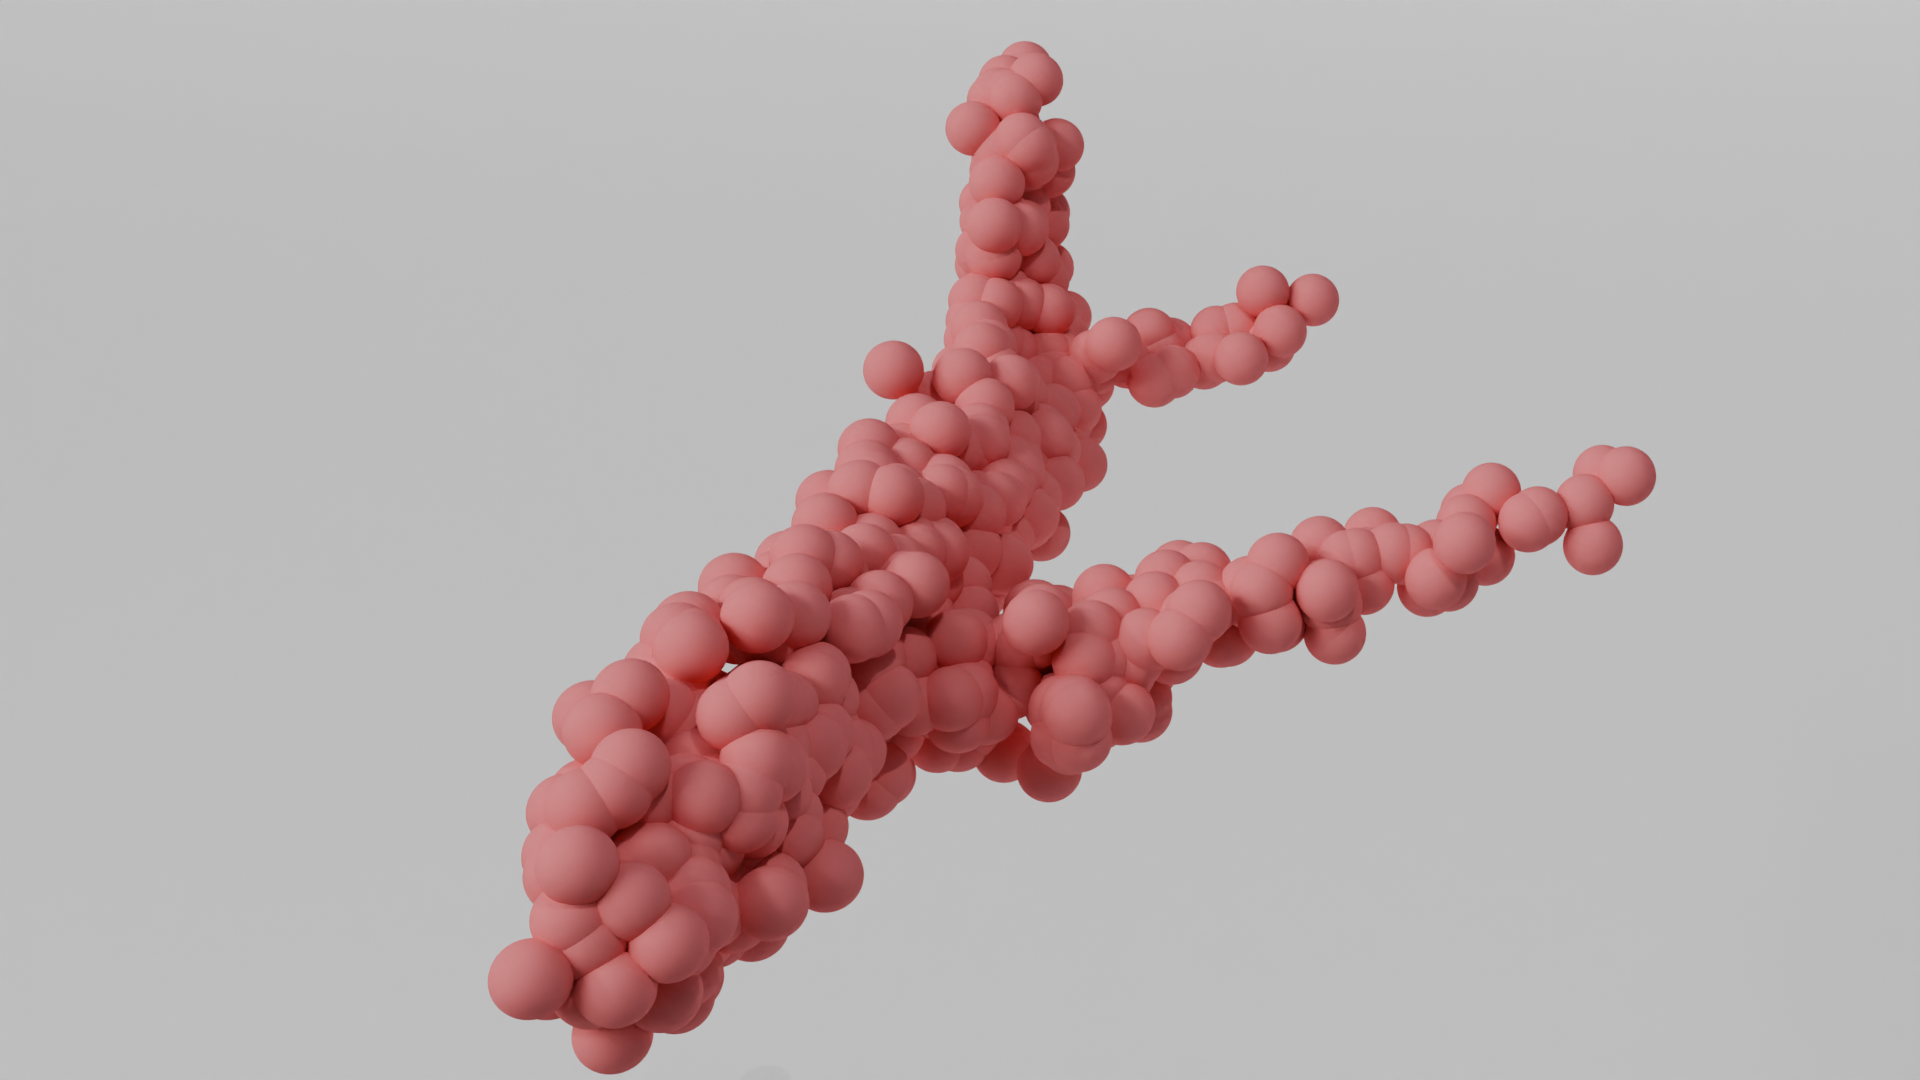
\includegraphics[width=\dimexpr\linewidth-20pt\relax]{figures/part_ap1.png}
        \makebox[20pt]{\raisebox{30pt}{\rotatebox[origin=c]{90}{\small DropCon}}}%
        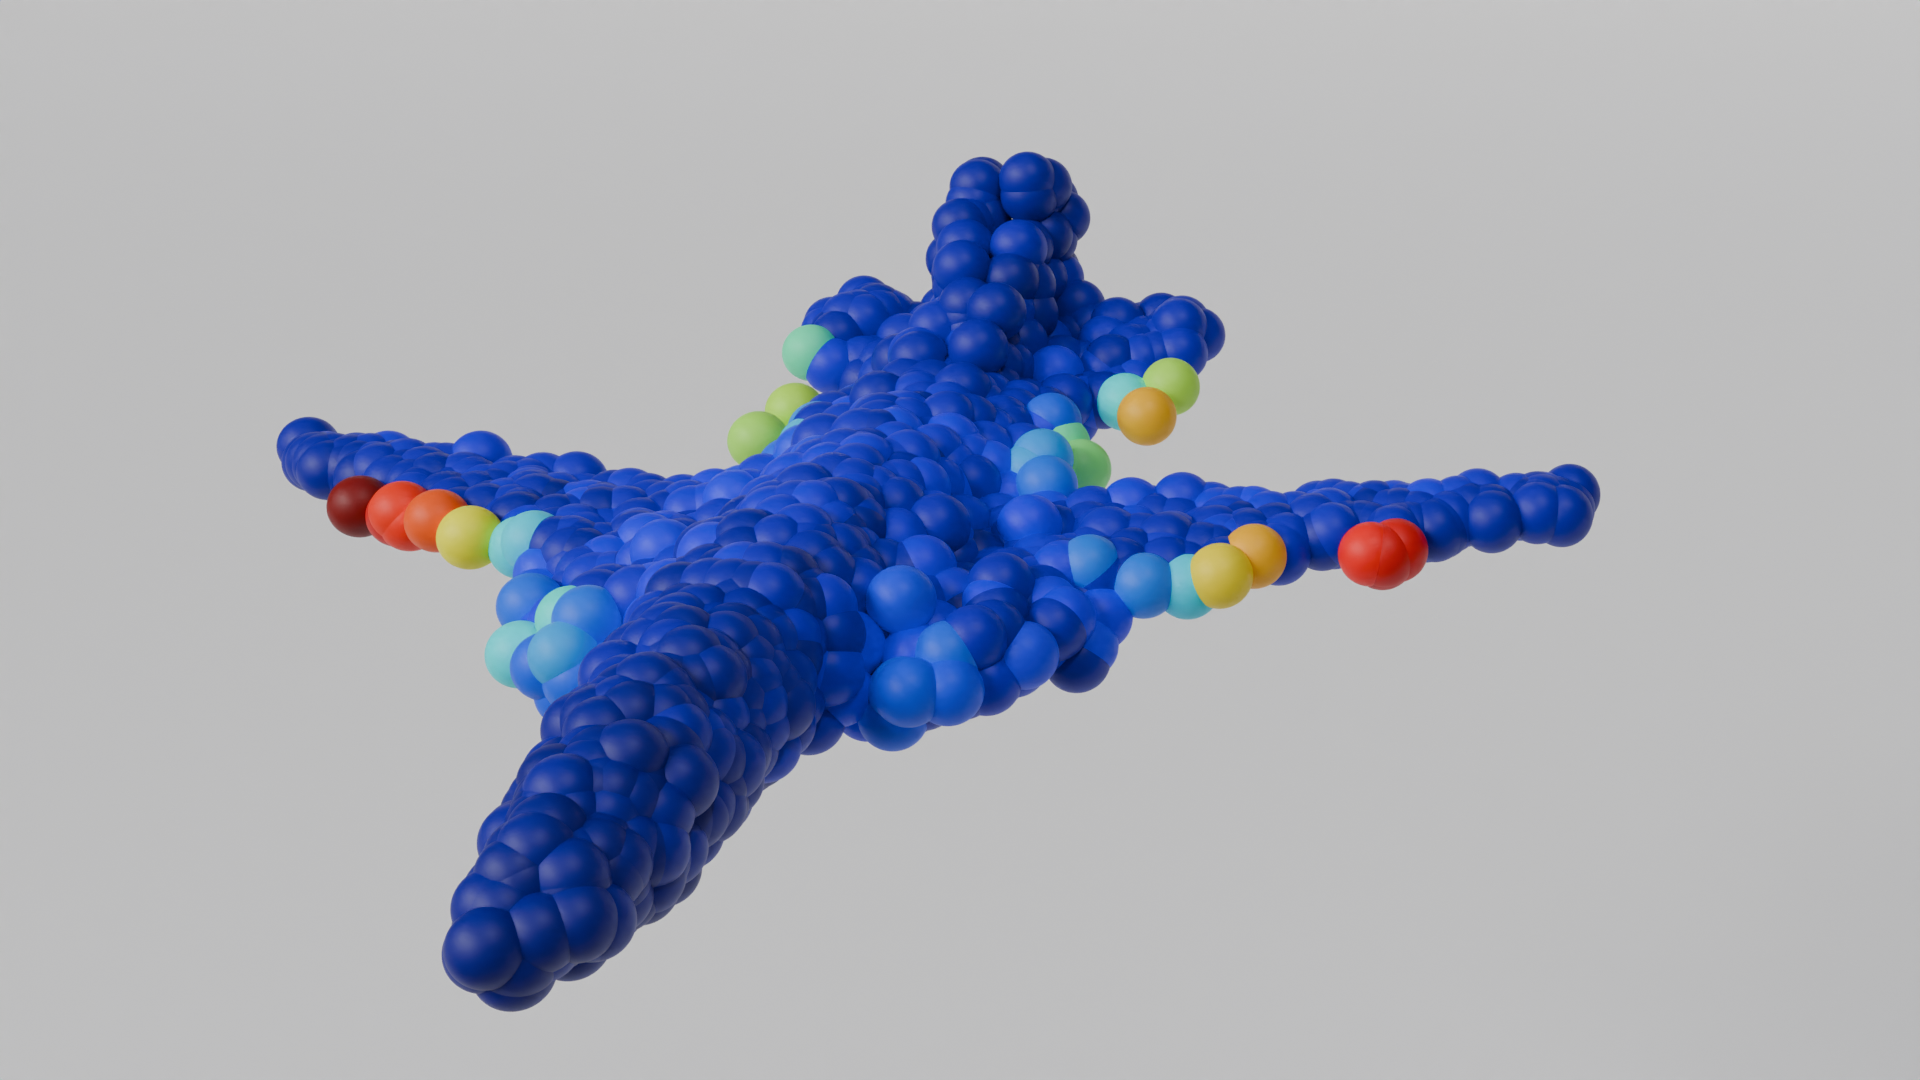
\includegraphics[width=\dimexpr\linewidth-20pt\relax]{figures/dc_lin_ap1.png}
        \makebox[20pt]{\raisebox{30pt}{\rotatebox[origin=c]{90}{\small Dropout}}}%
        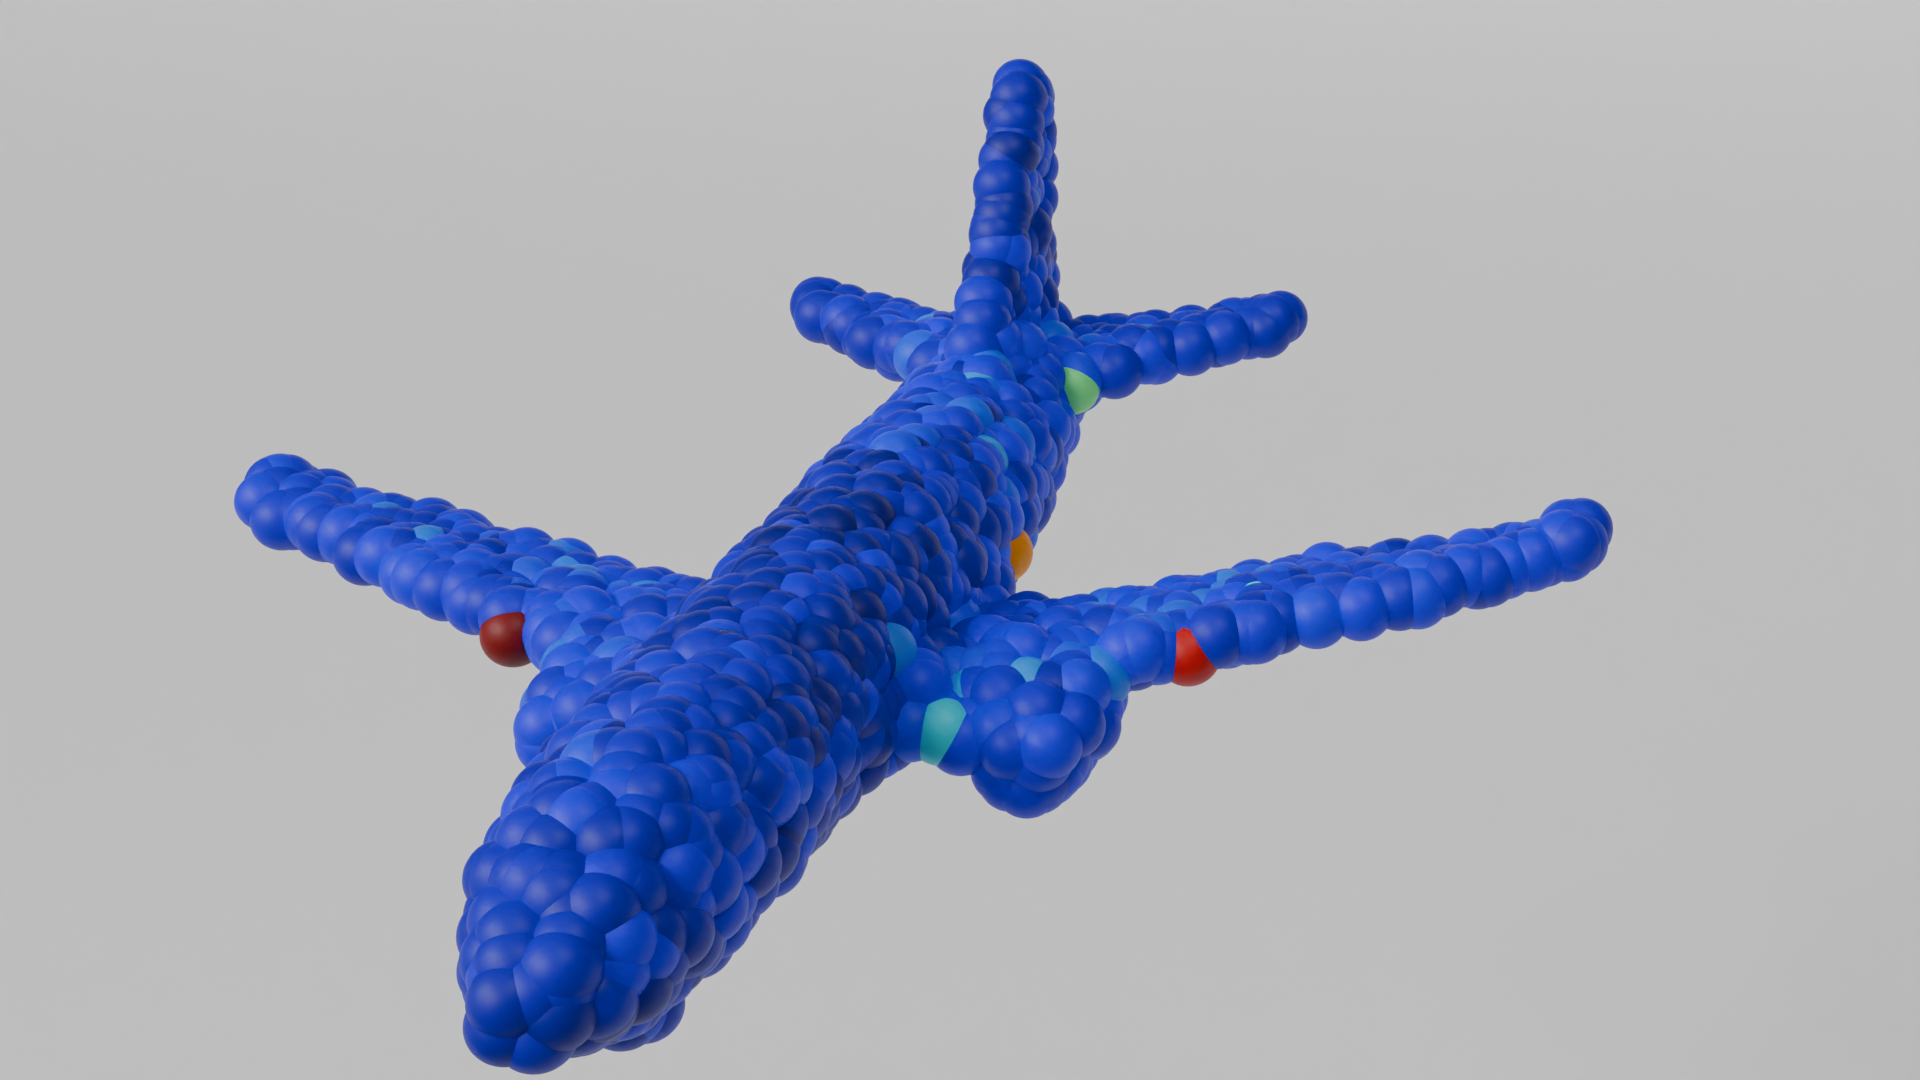
\includegraphics[width=\dimexpr\linewidth-20pt\relax]{figures/do_lin_ap1.png}
        \makebox[20pt]{\raisebox{30pt}{\rotatebox[origin=c]{90}{\small Ensemble}}}%
        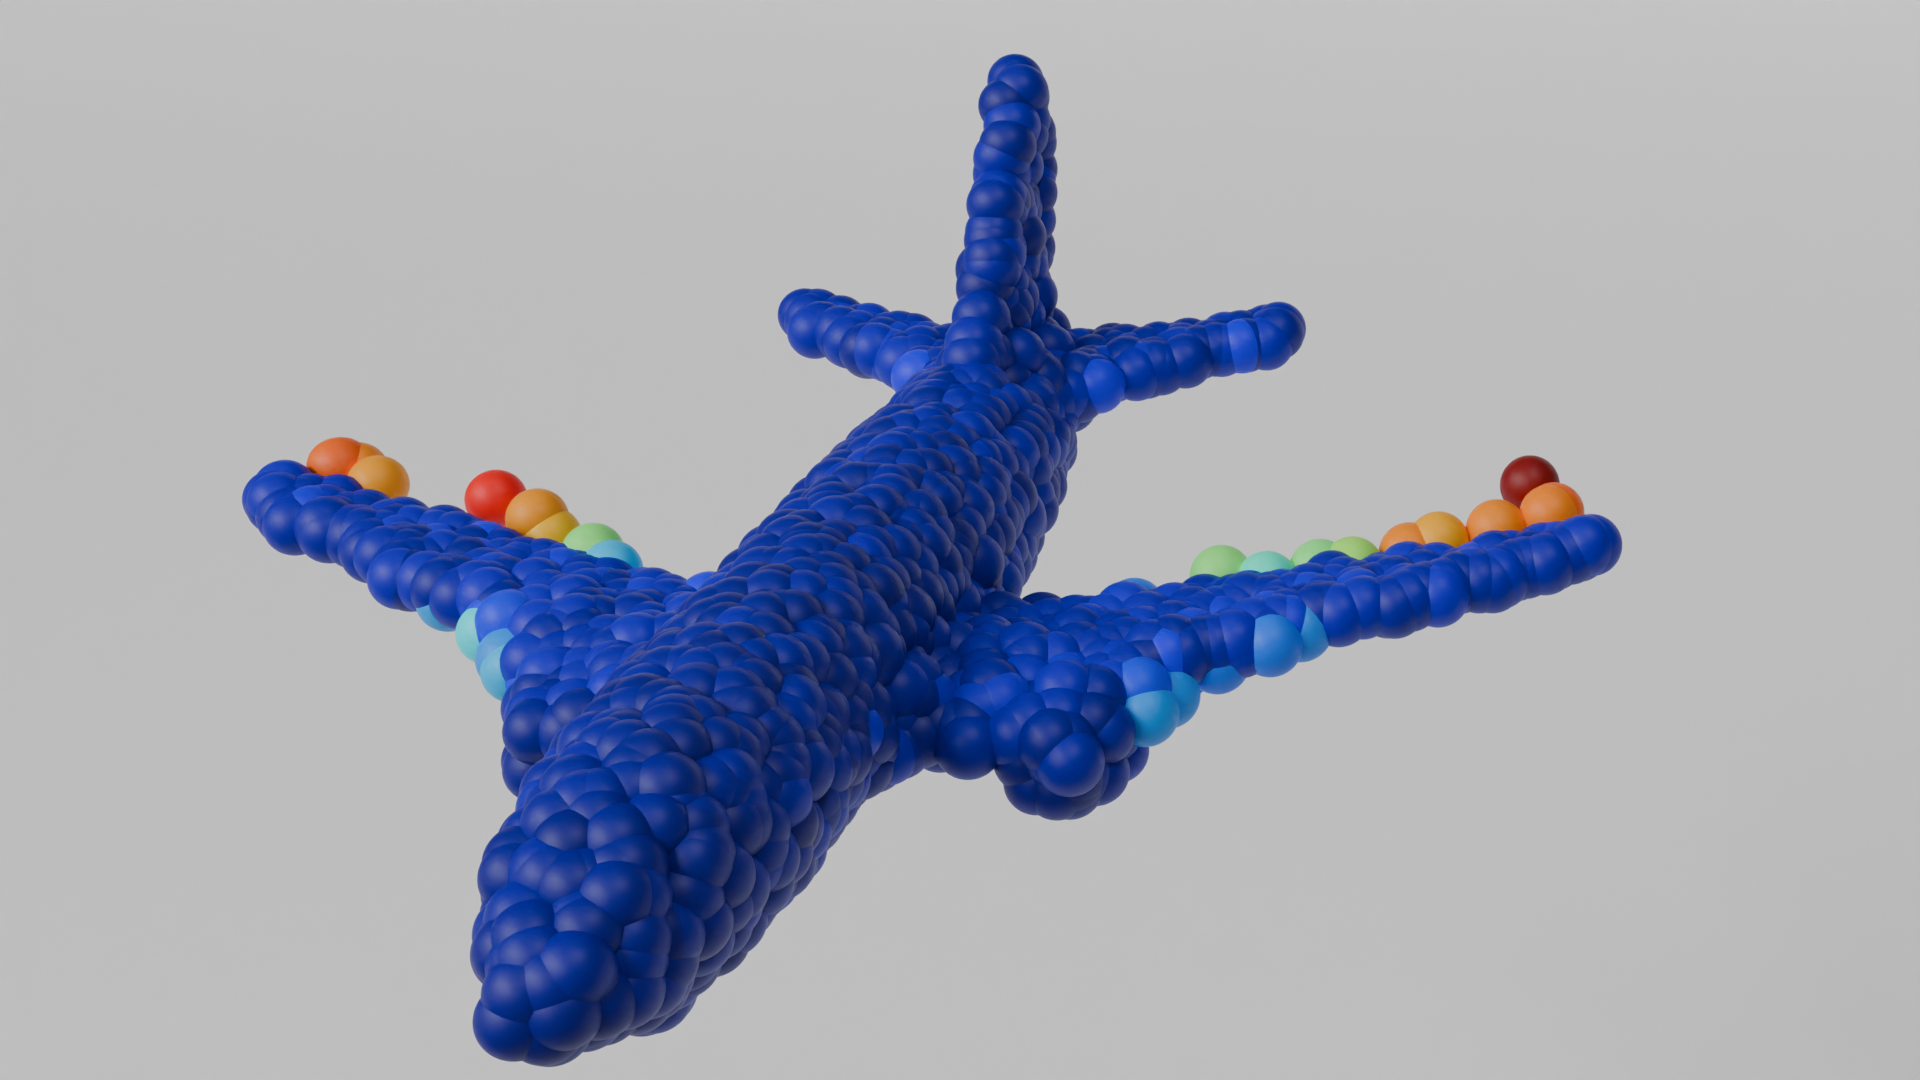
\includegraphics[width=\dimexpr\linewidth-20pt\relax]{figures/ens_lin_ap1.png}
        \makebox[20pt]{\raisebox{30pt}{\rotatebox[origin=c]{90}{\small Implicit}}}%
        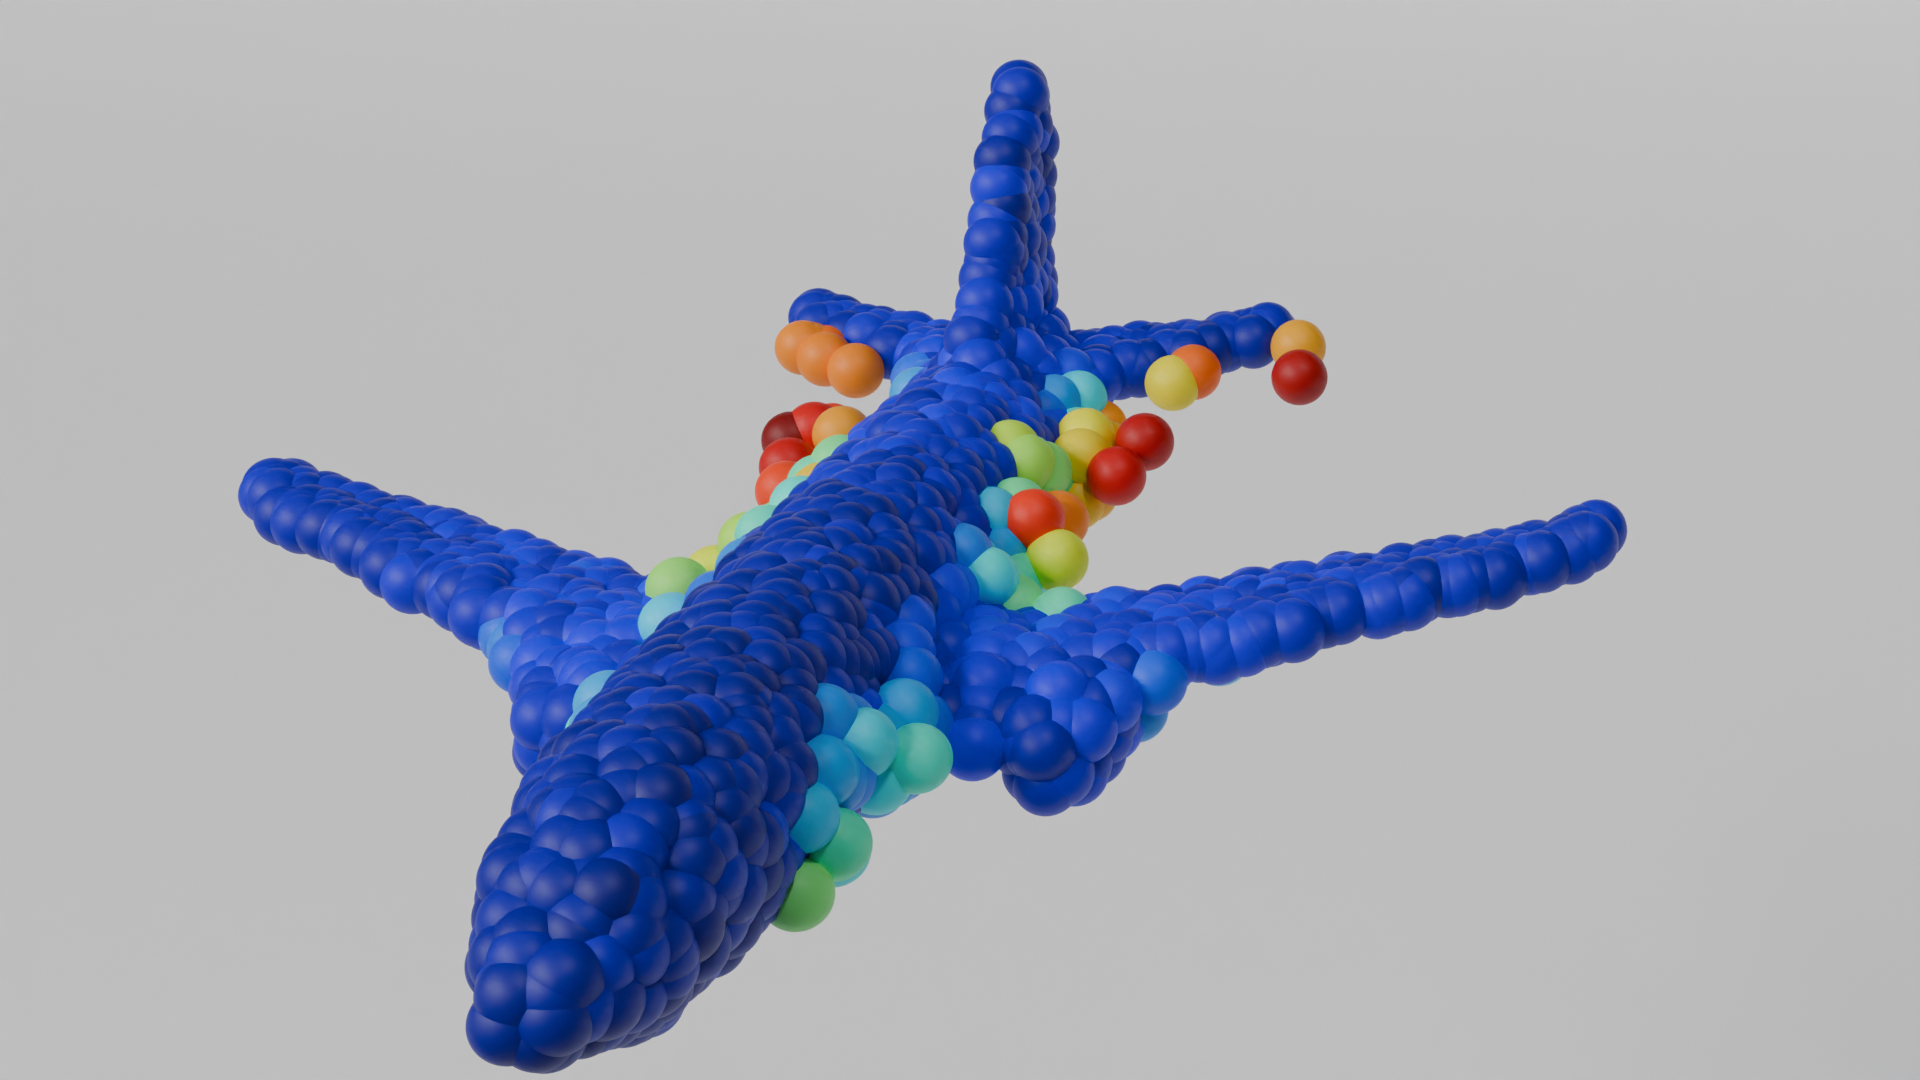
\includegraphics[width=\dimexpr\linewidth-20pt\relax]{figures/iml_lin_ap1.png}
        \makebox[20pt]{\raisebox{30pt}{\rotatebox[origin=c]{90}{\small GT}}}%
        \includegraphics[width=\dimexpr\linewidth-20pt\relax]{figures/com_ap1.png}
        \caption{Airplane 1}
    \end{subfigure}\hfill
    \begin{subfigure}[t]{0.315\textwidth}
        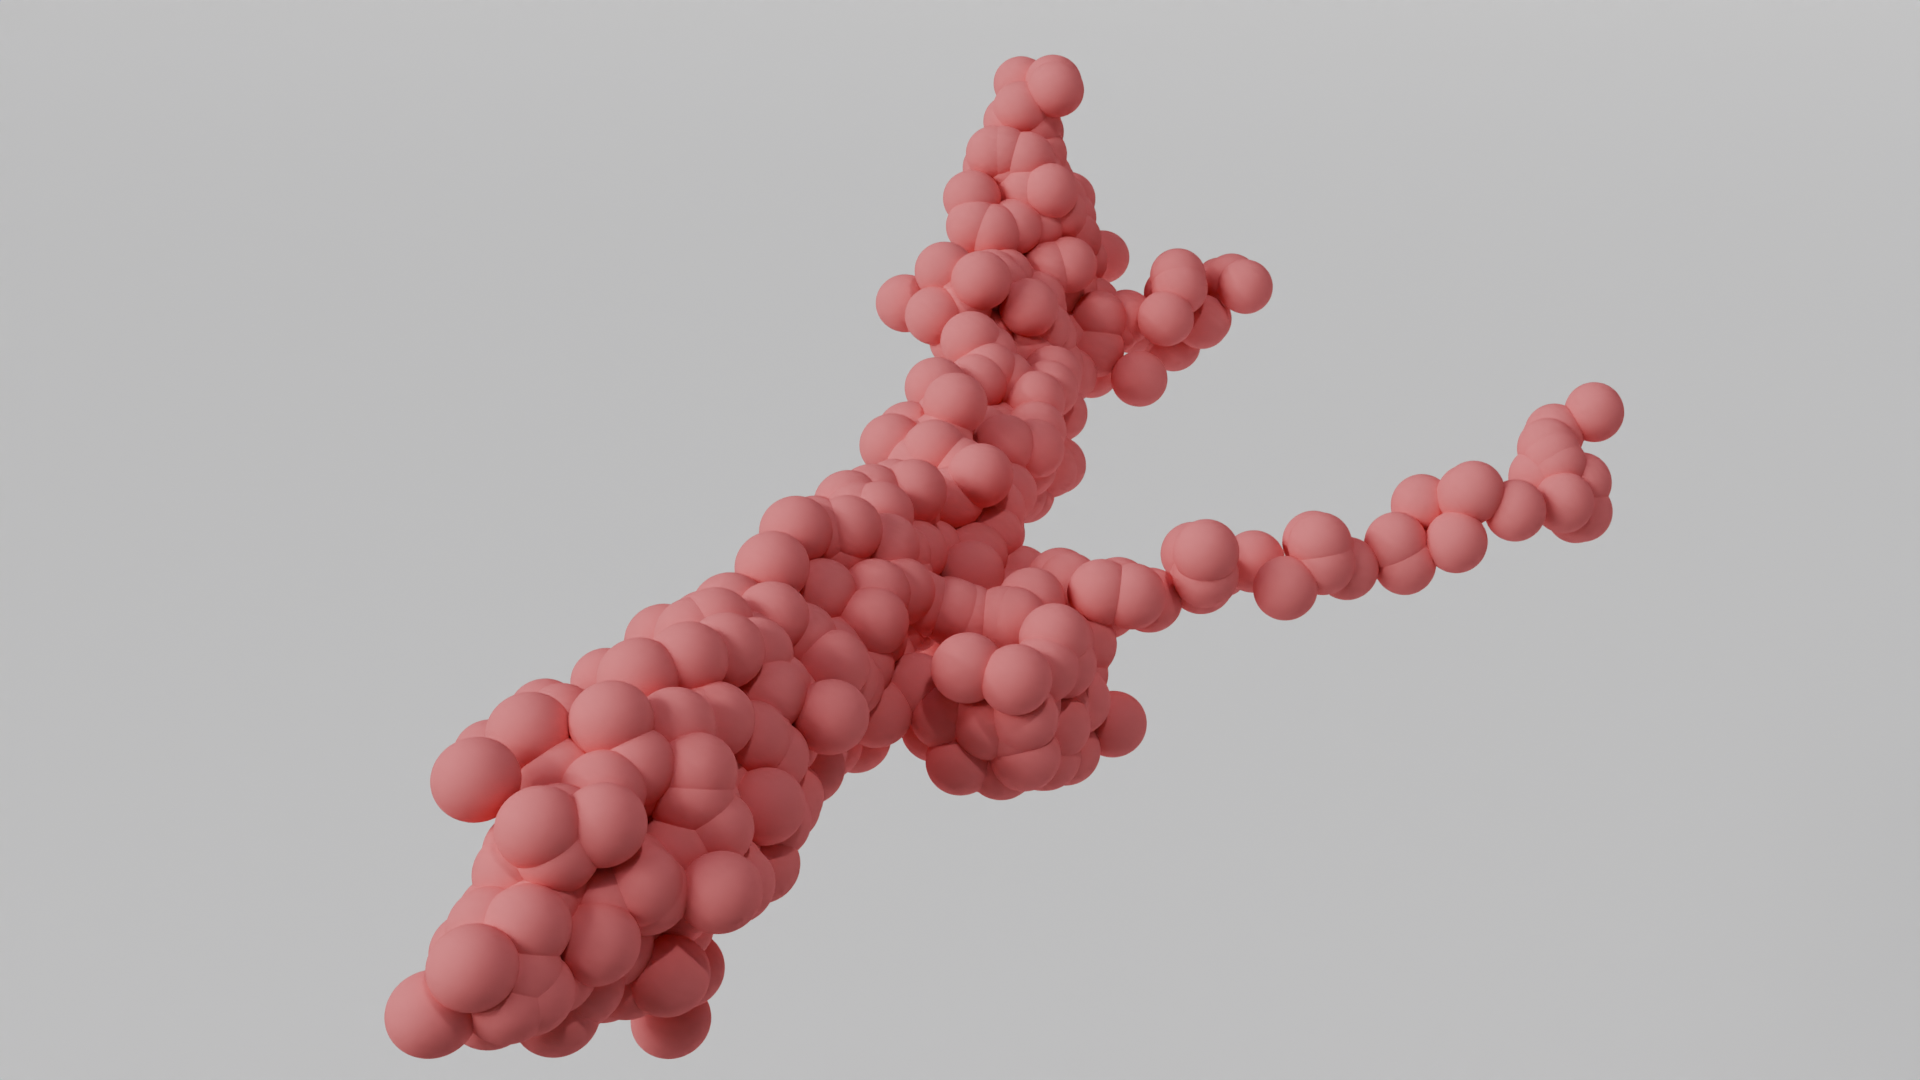
\includegraphics[width=\textwidth]{figures/part_ap2.png}
        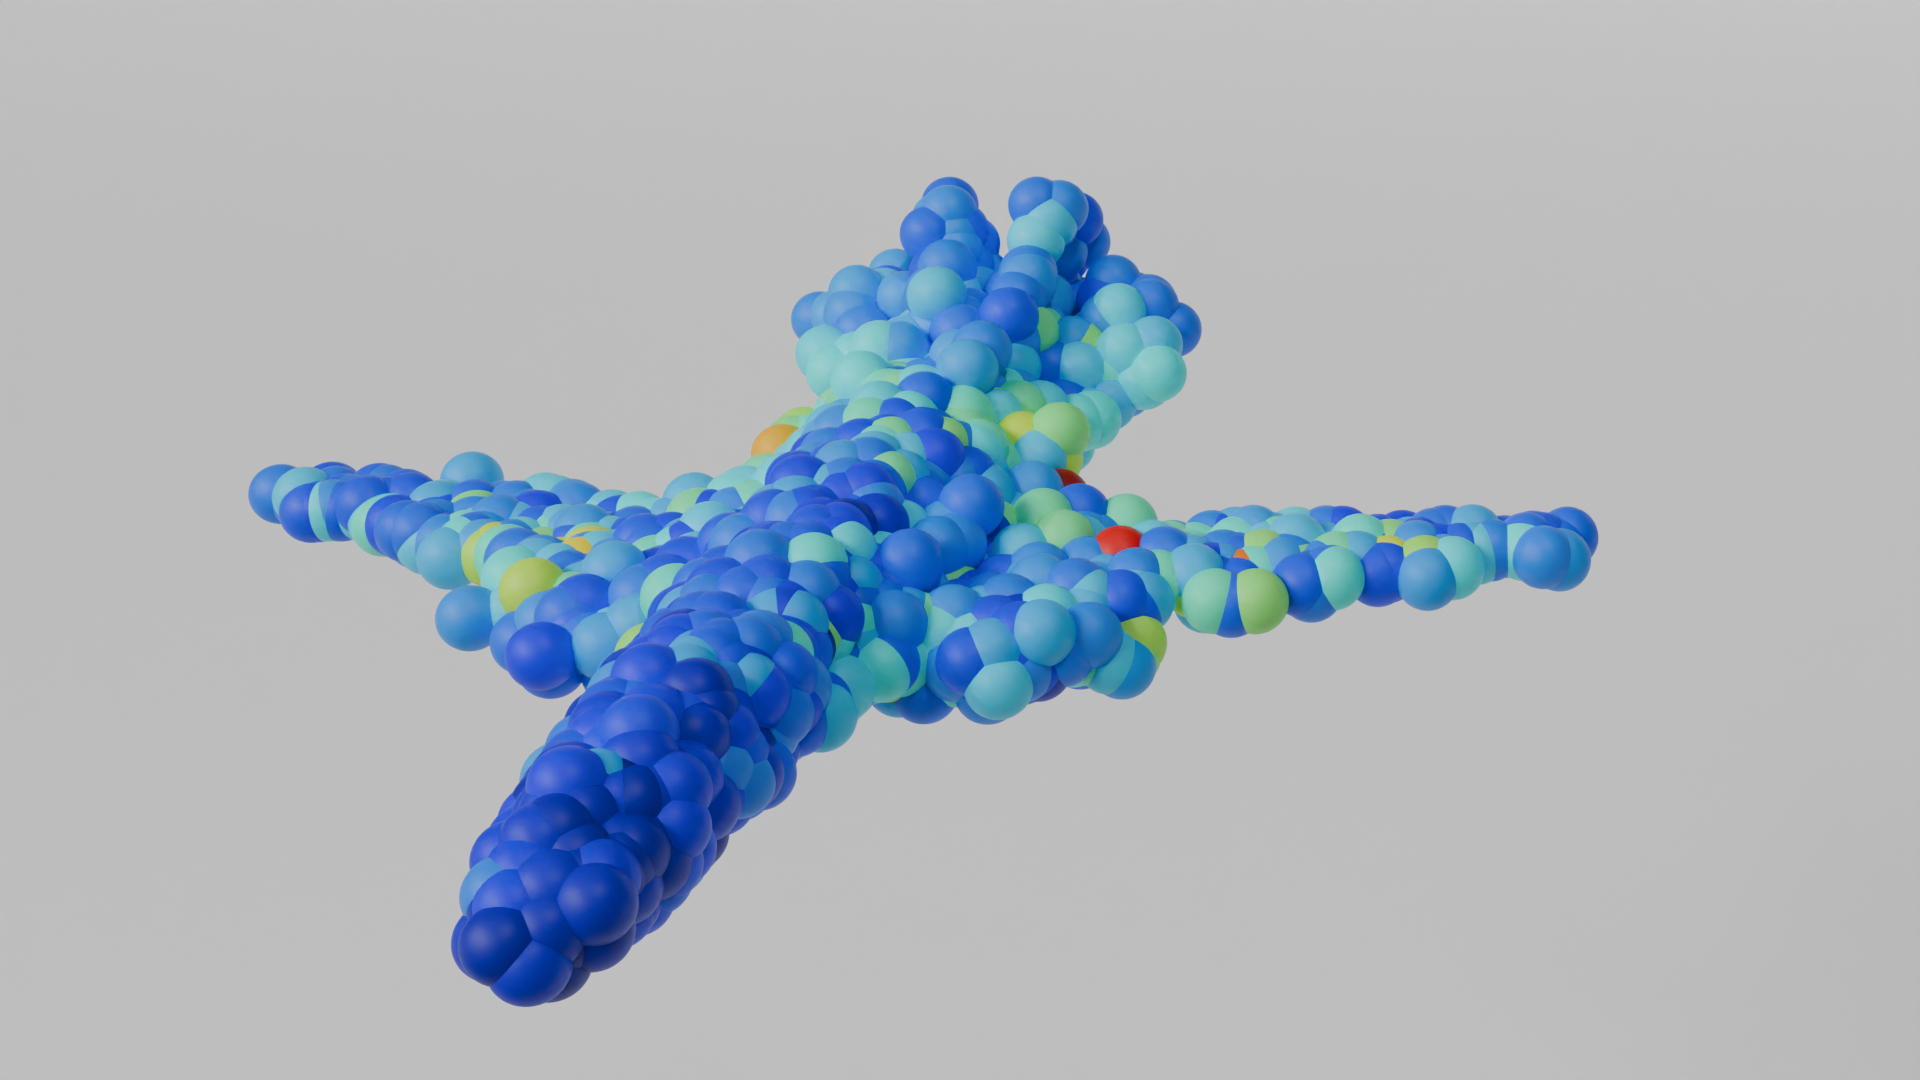
\includegraphics[width=\textwidth]{figures/dc_lin_ap2.png}
        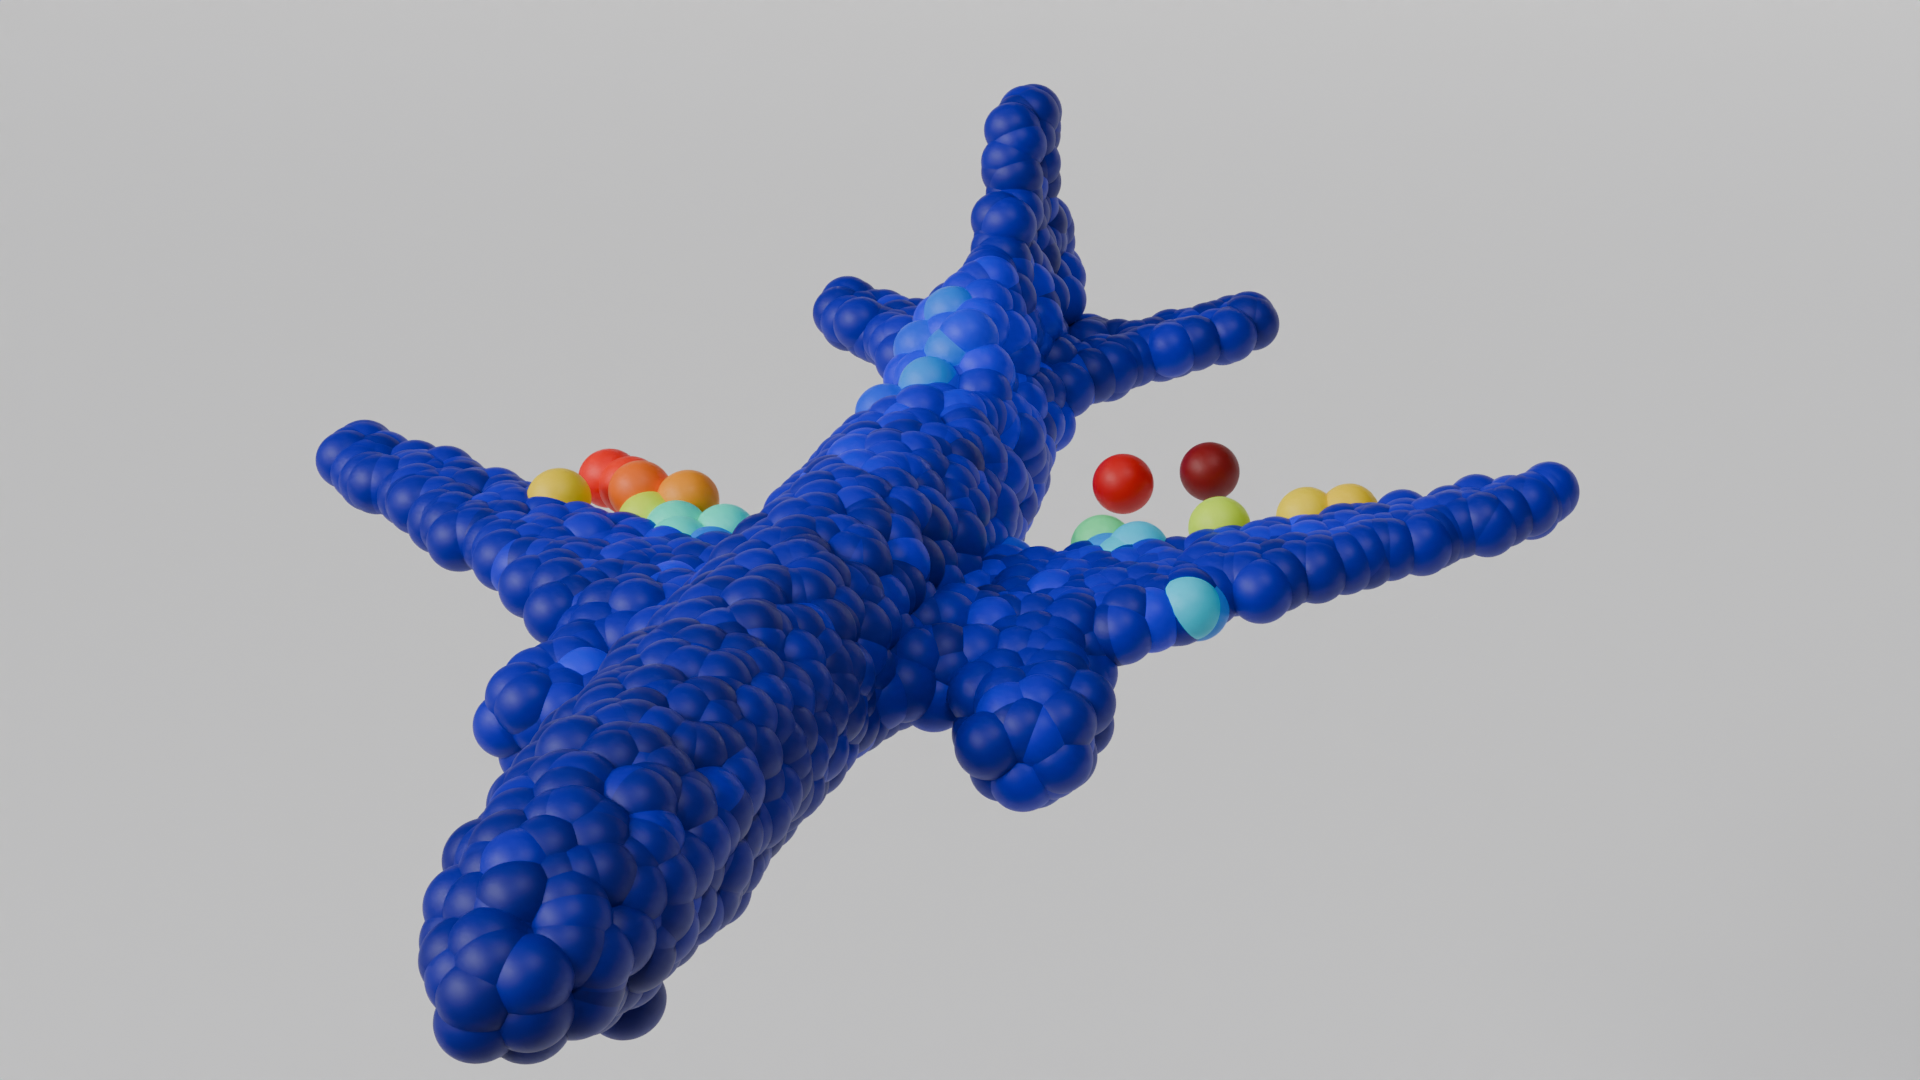
\includegraphics[width=\textwidth]{figures/do_lin_ap2.png}
        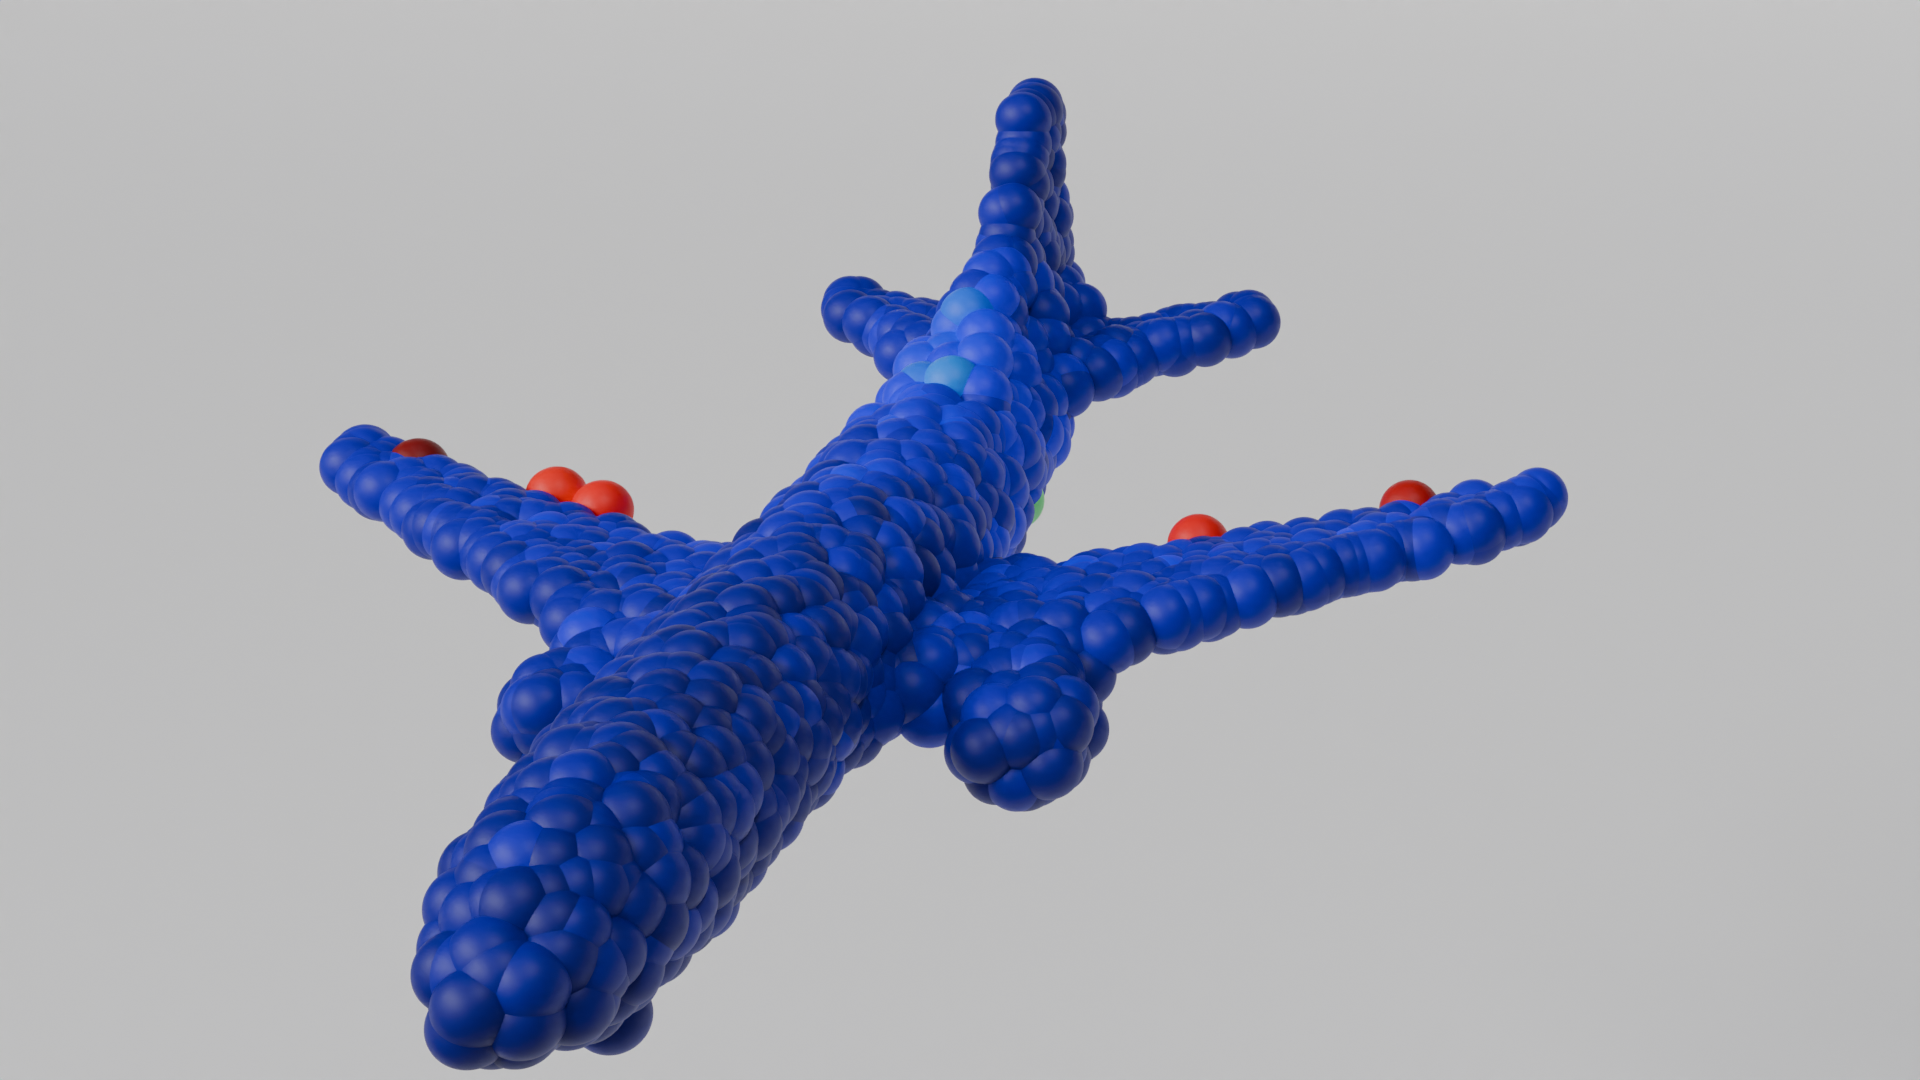
\includegraphics[width=\textwidth]{figures/ens_lin_ap2.png}
        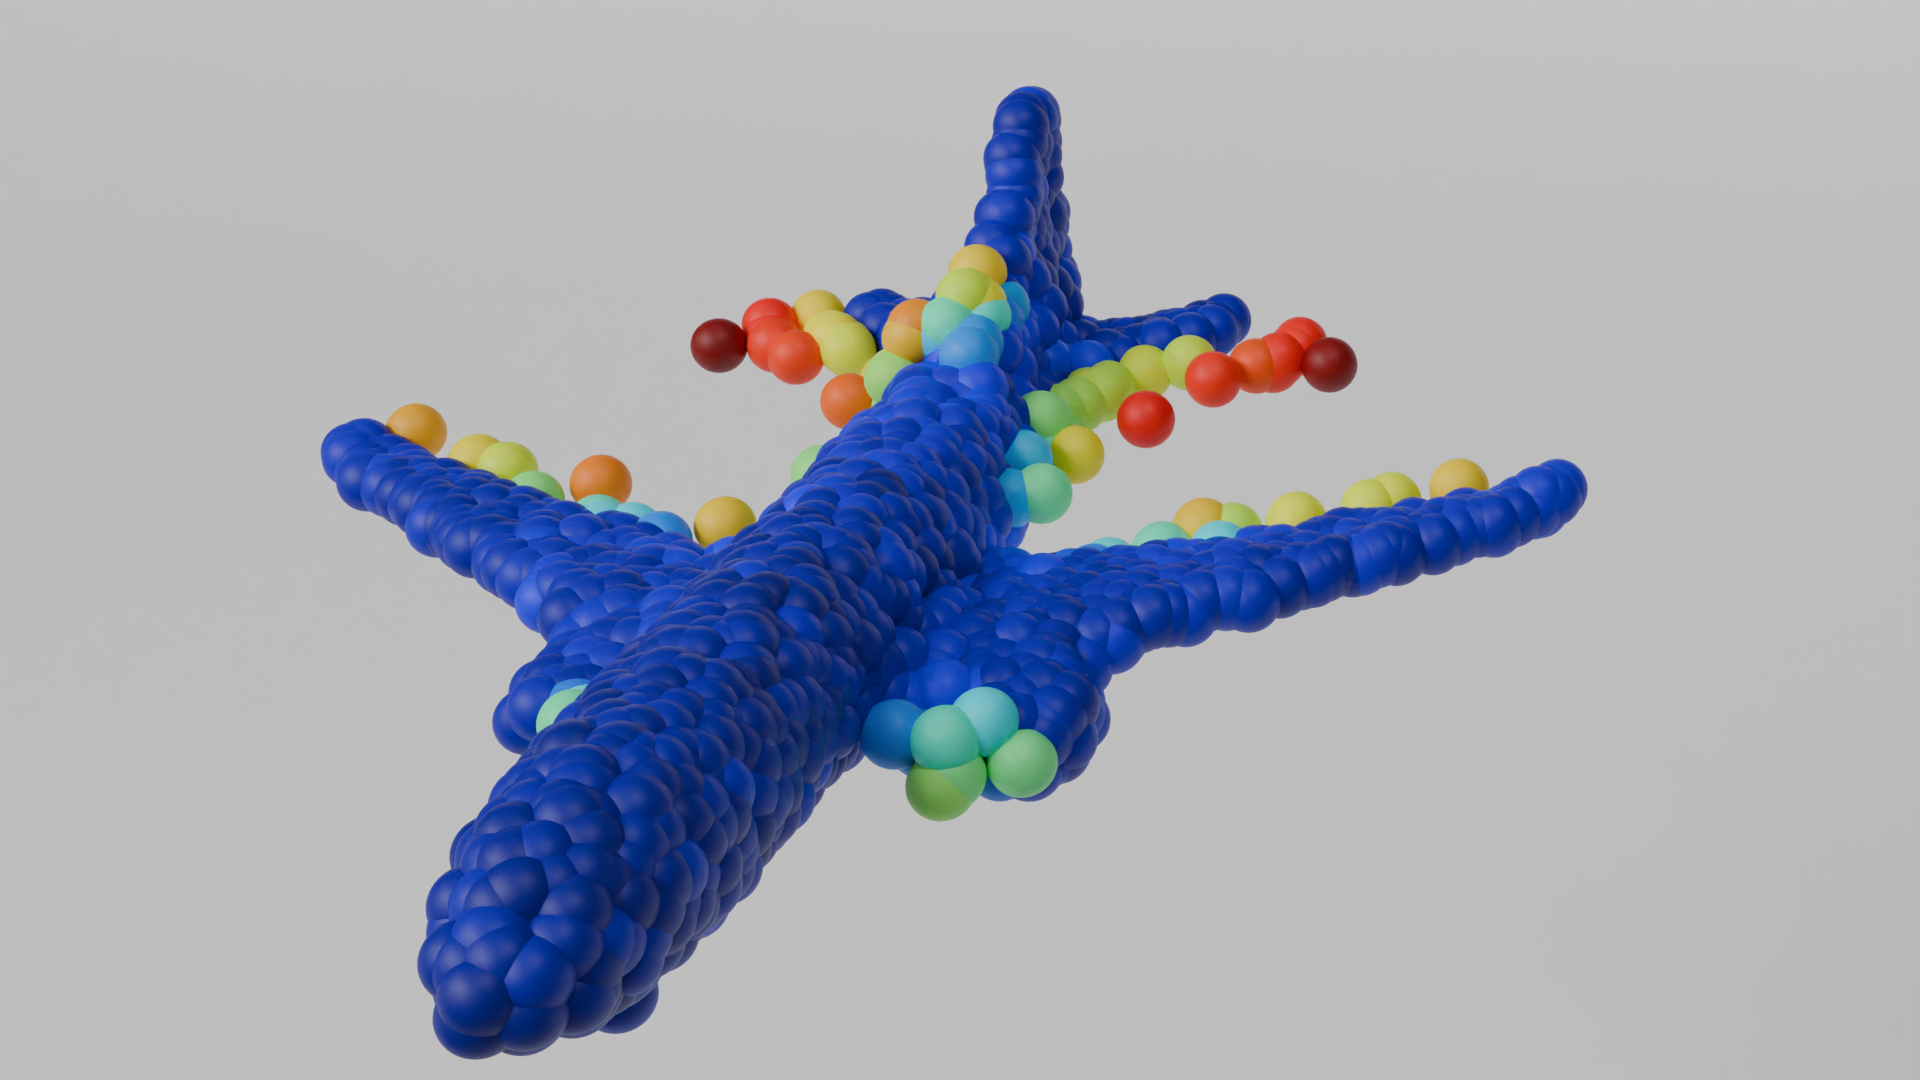
\includegraphics[width=\textwidth]{figures/iml_lin_ap2.png}
        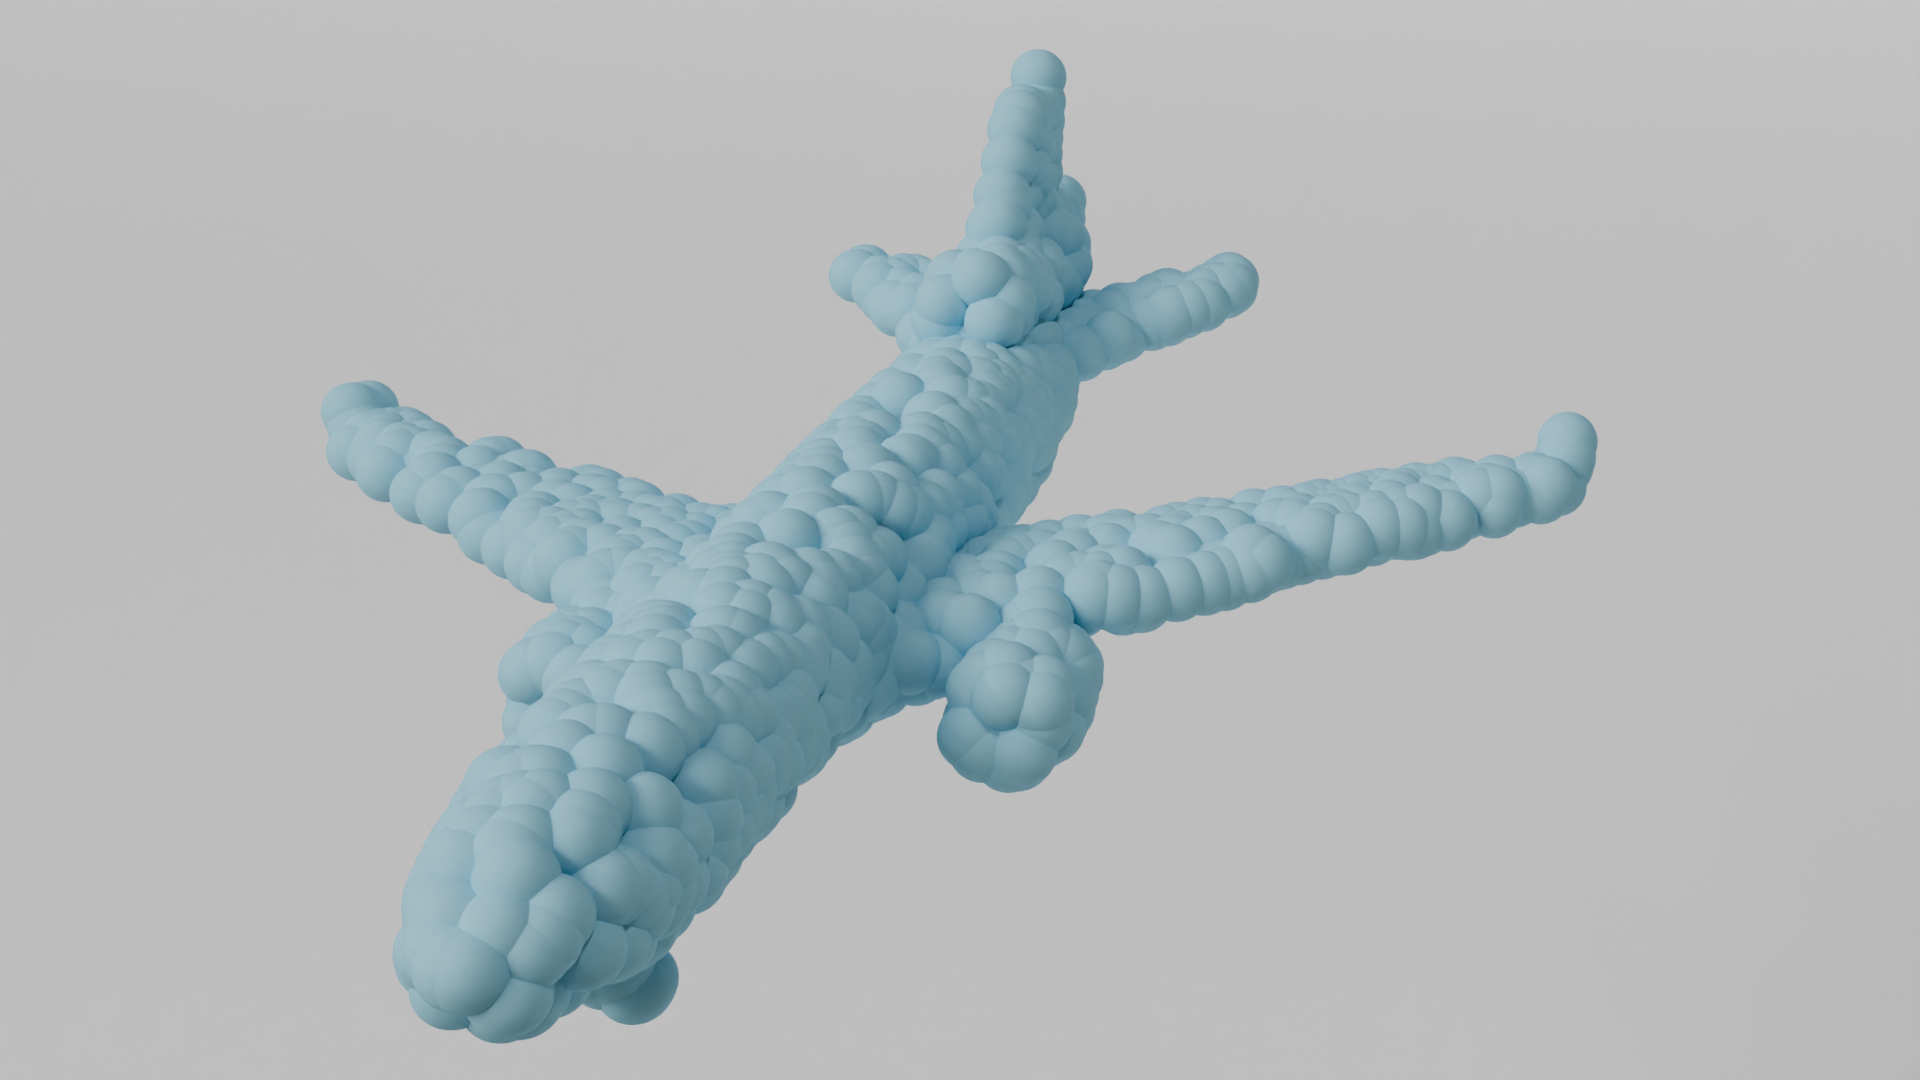
\includegraphics[width=\textwidth]{figures/com_ap2.png}
        \caption{Airplane 2}
    \end{subfigure}\hfill
    \begin{subfigure}[t]{0.315\textwidth}
        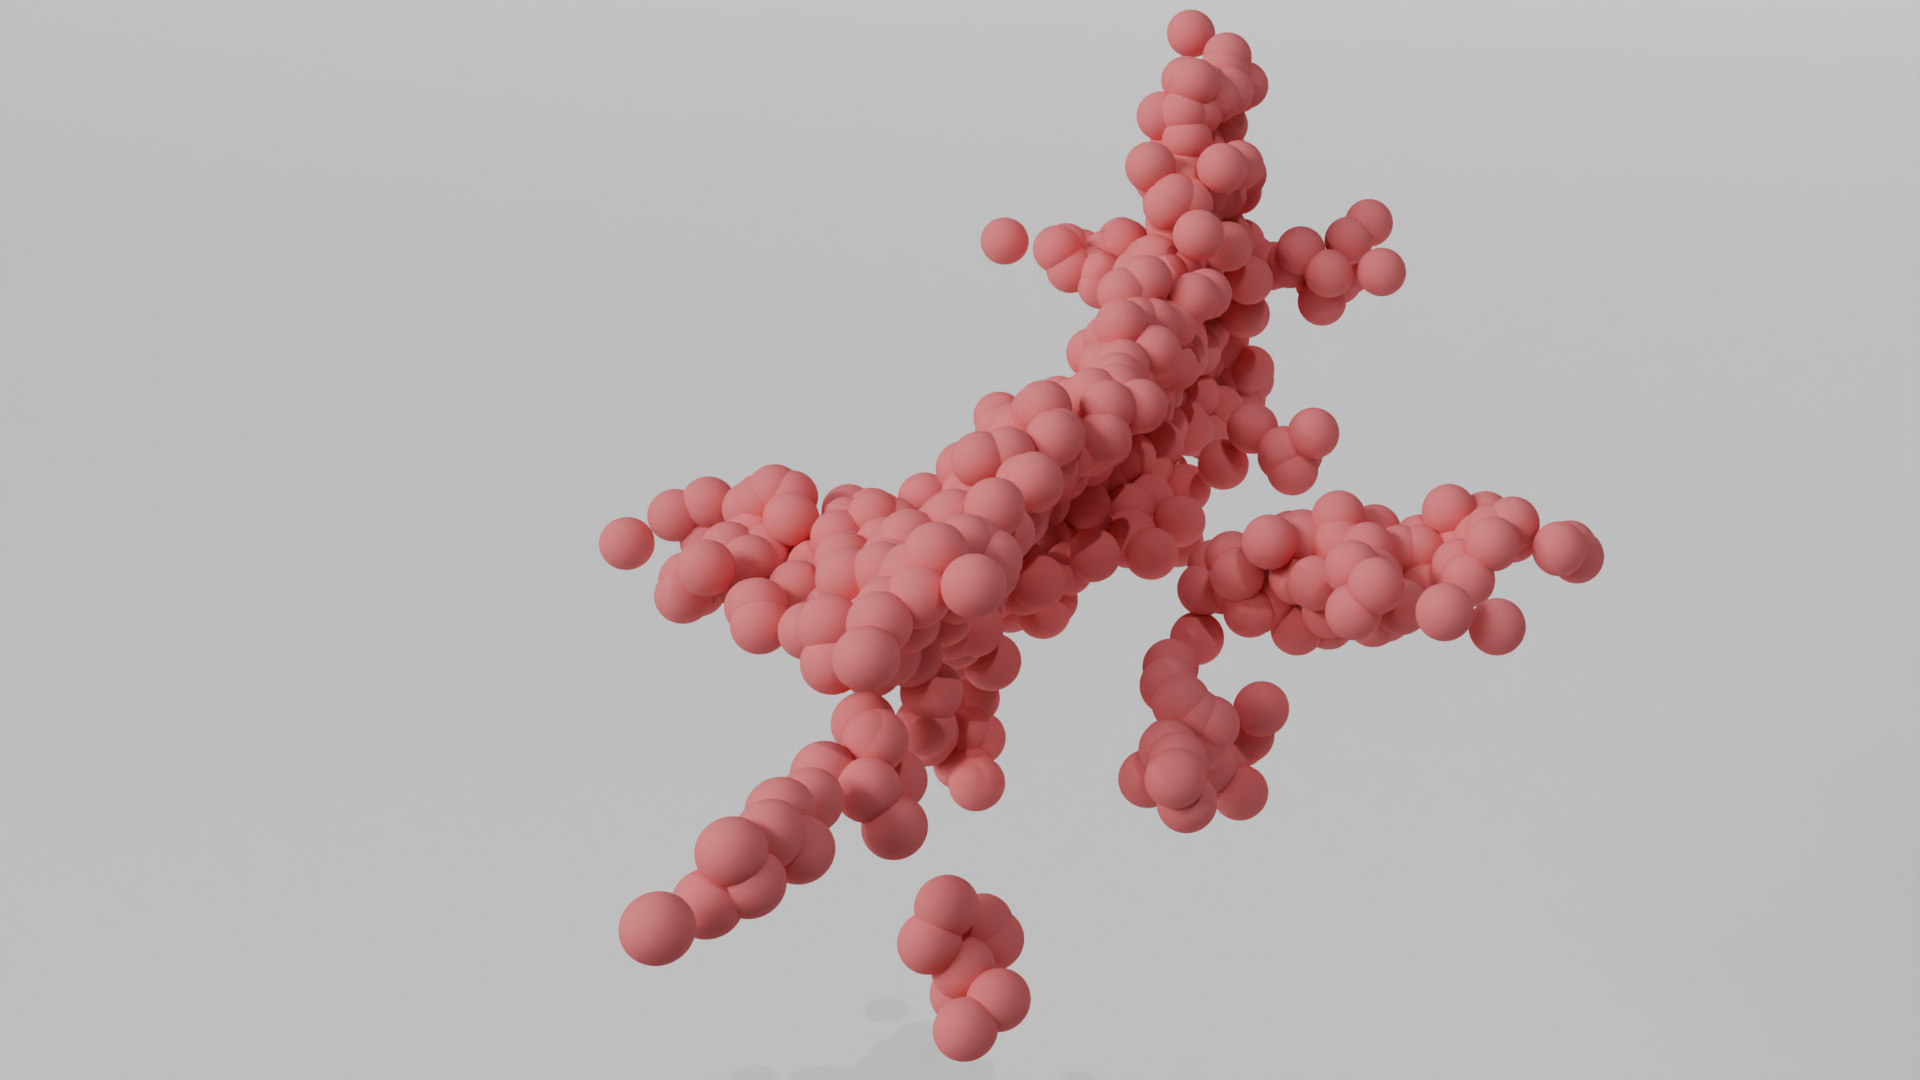
\includegraphics[width=\textwidth]{figures/part_ap3.png}
        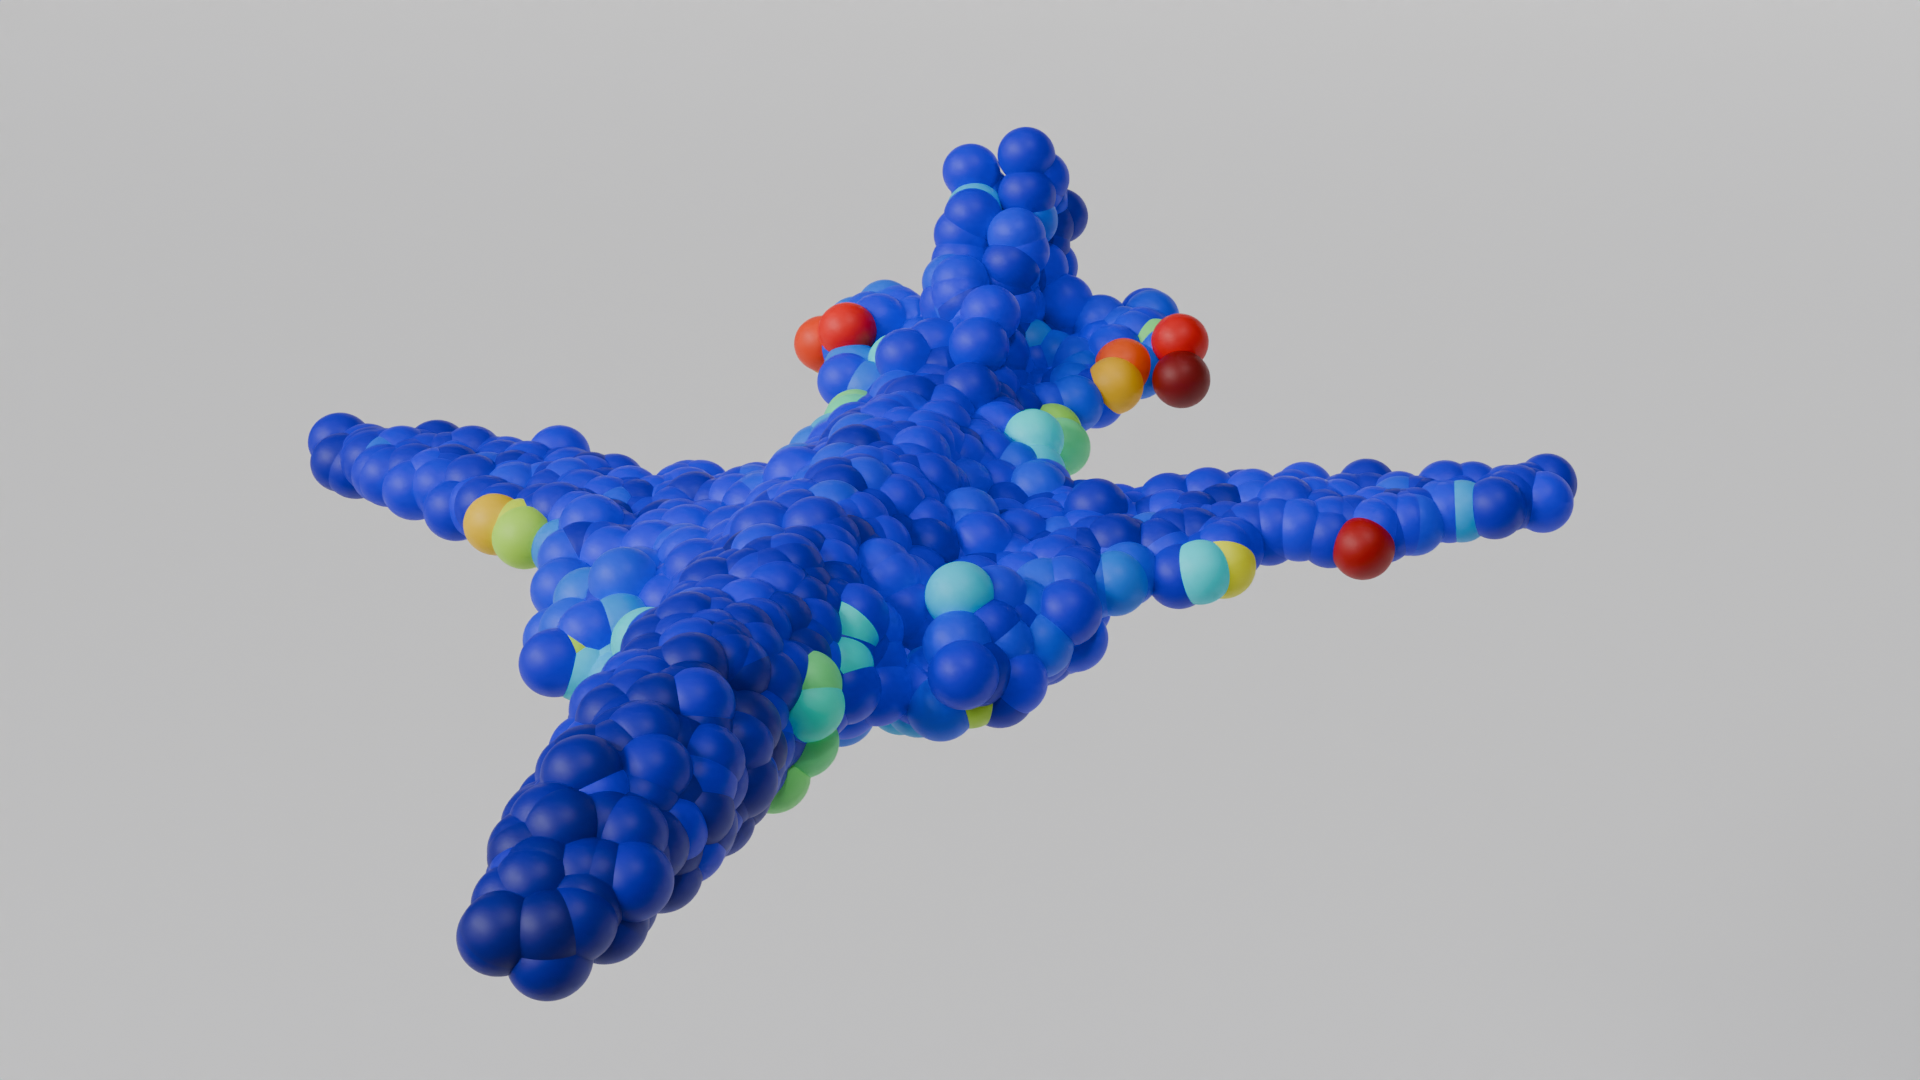
\includegraphics[width=\textwidth]{figures/dc_lin_ap3.png}
        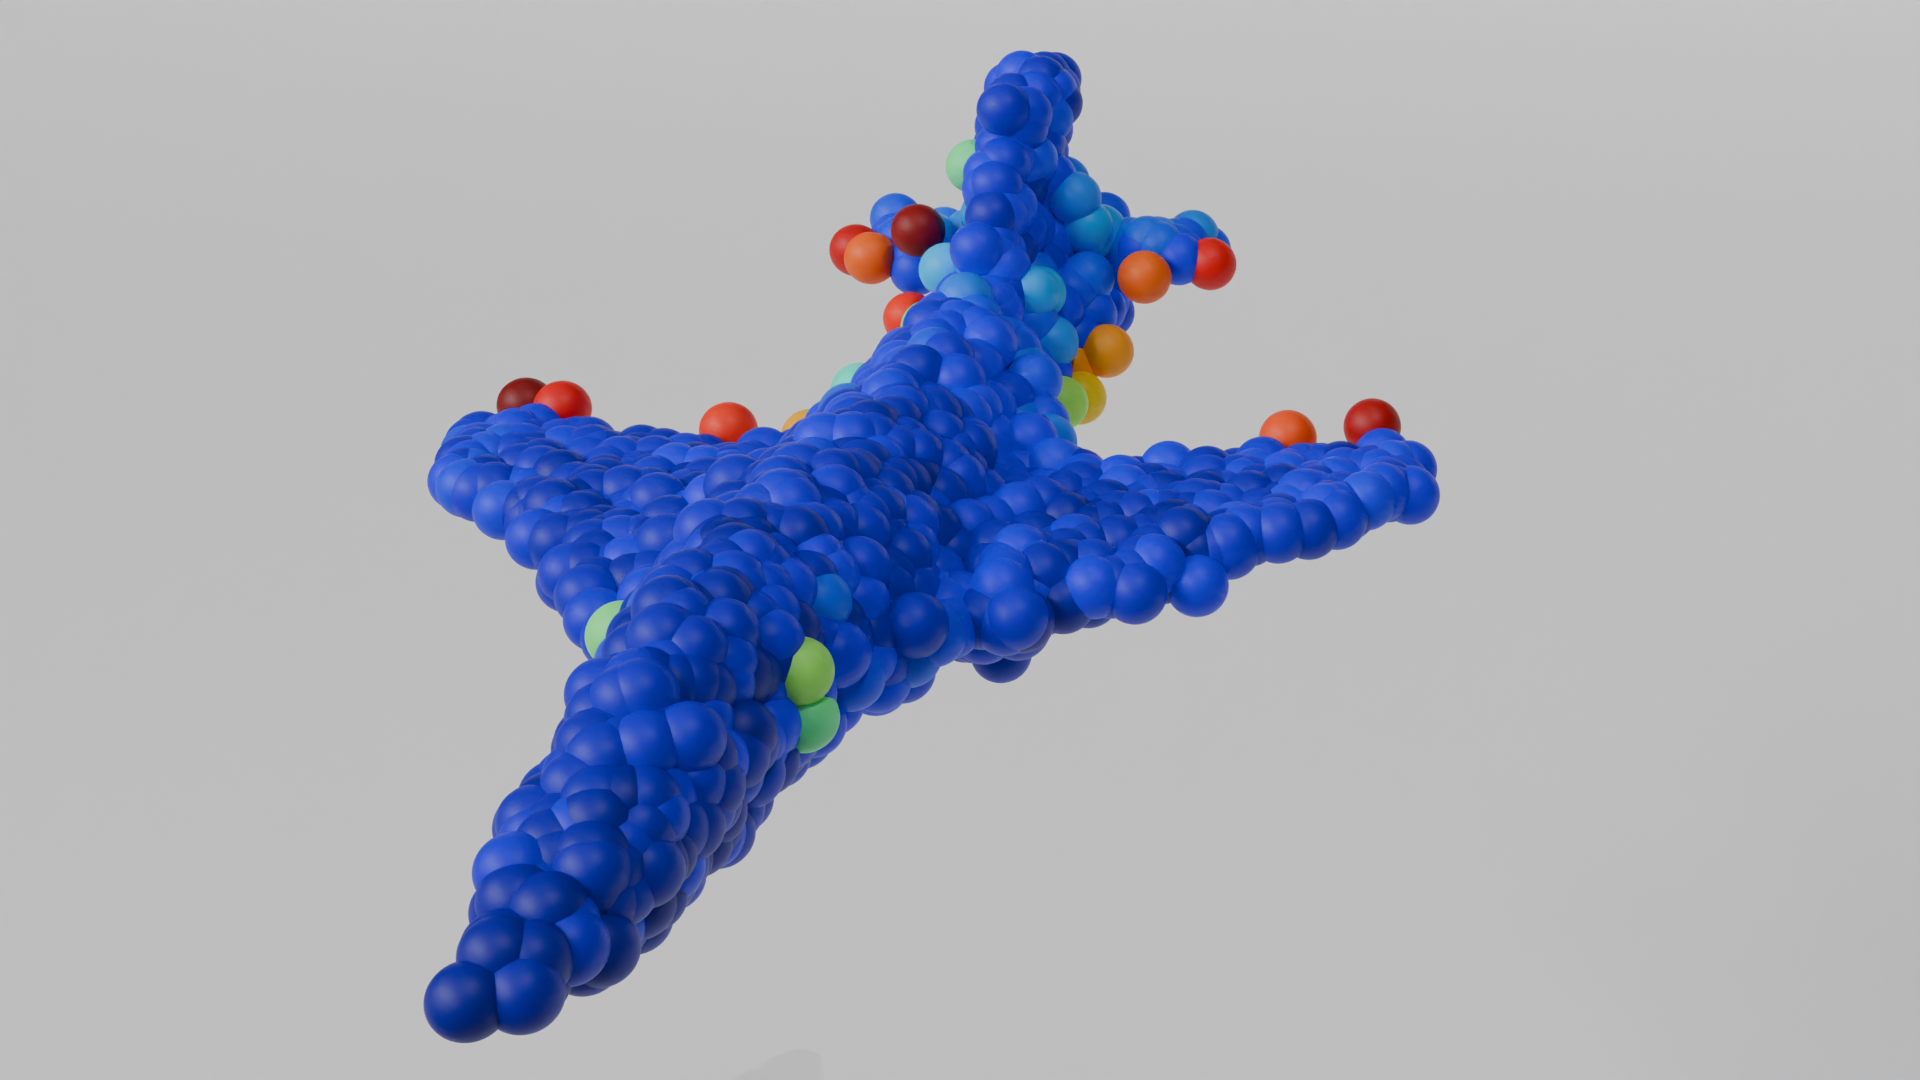
\includegraphics[width=\textwidth]{figures/do_lin_ap3.png}
        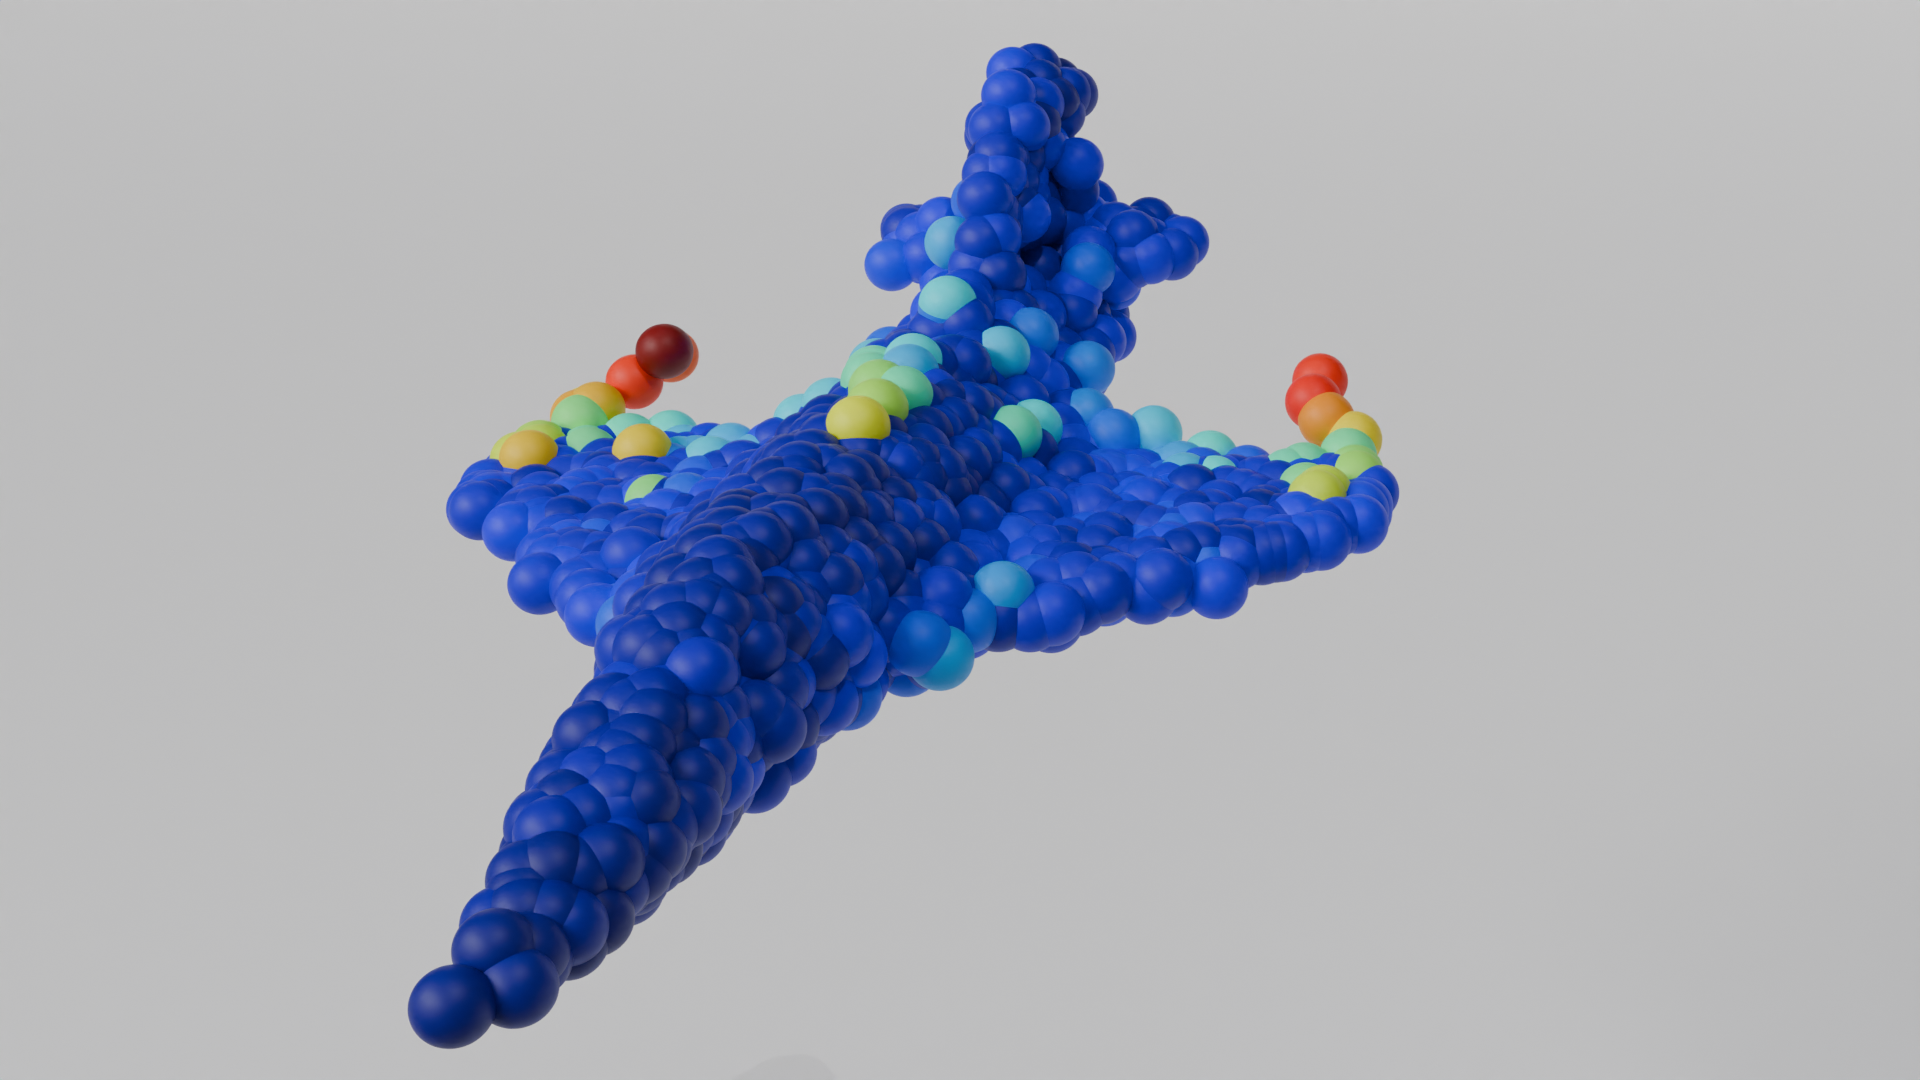
\includegraphics[width=\textwidth]{figures/ens_lin_ap3.png}
        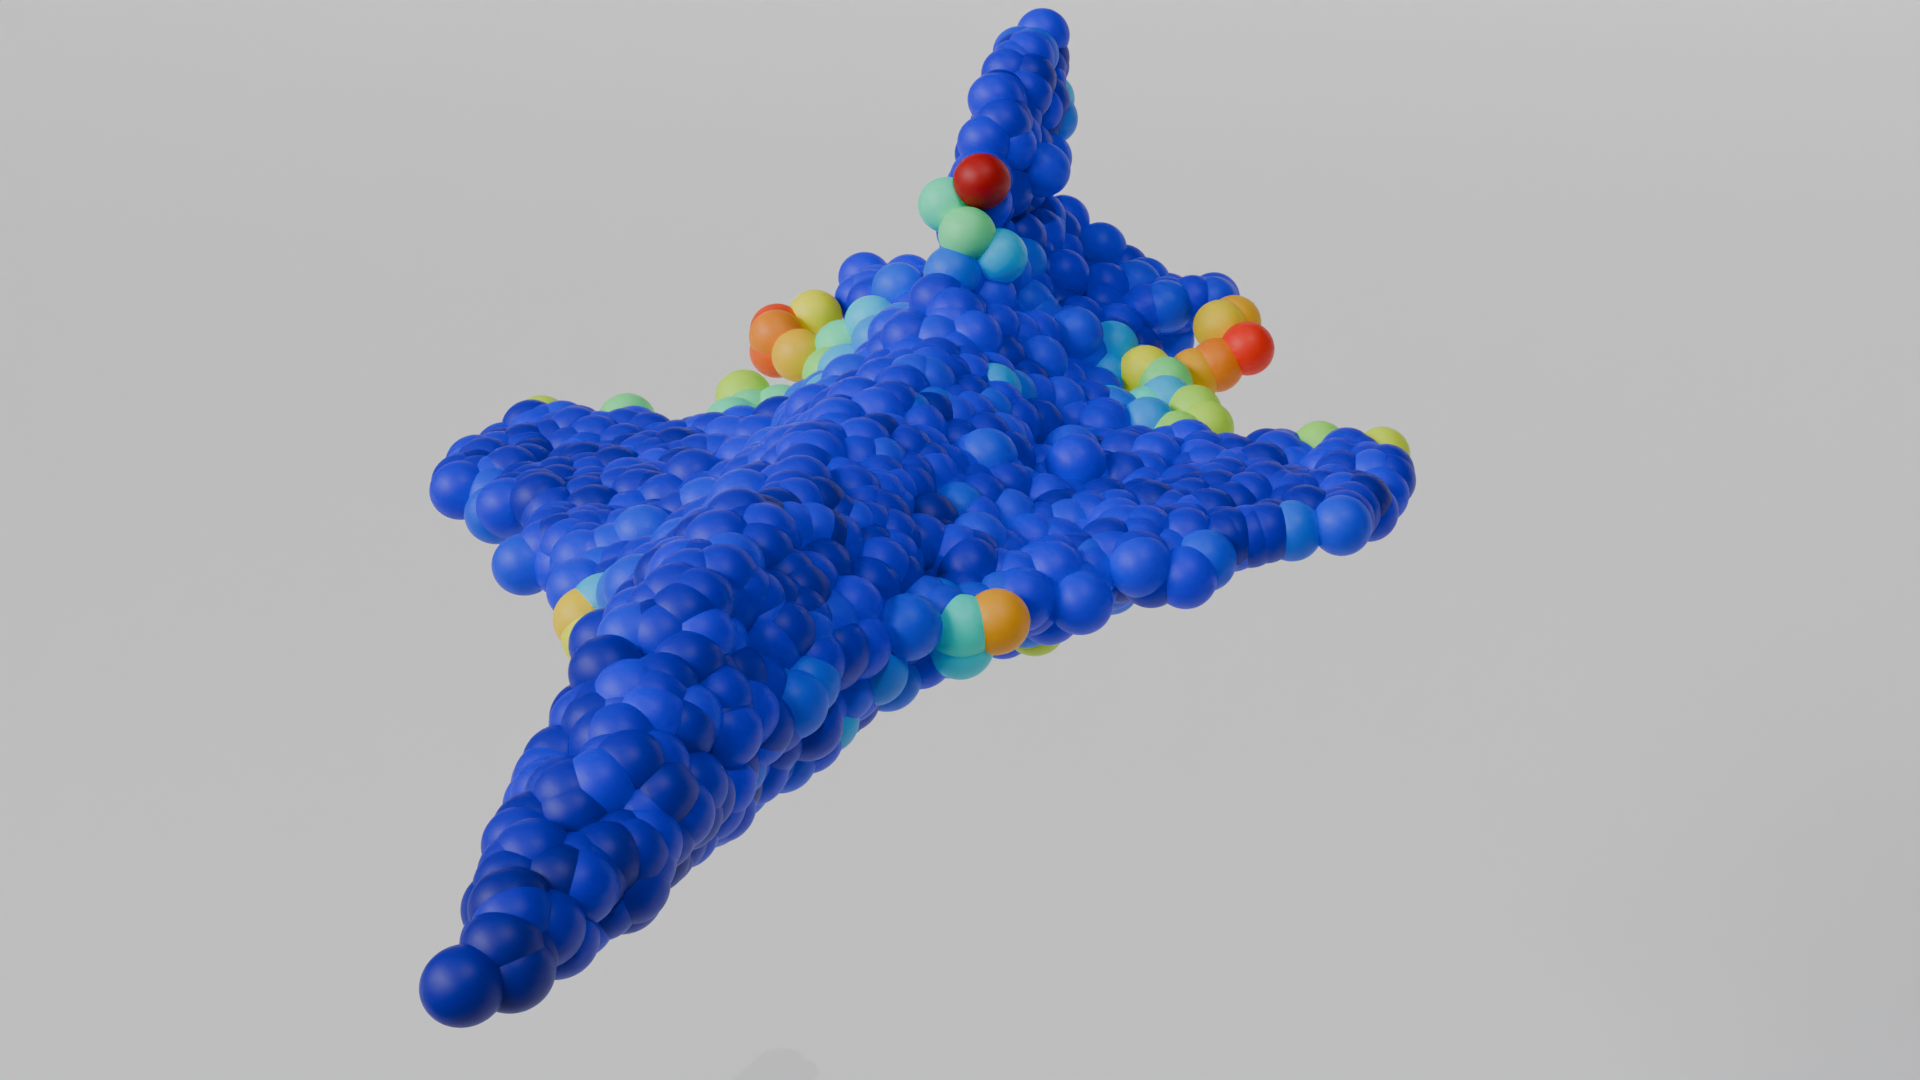
\includegraphics[width=\textwidth]{figures/iml_lin_ap3.png}
        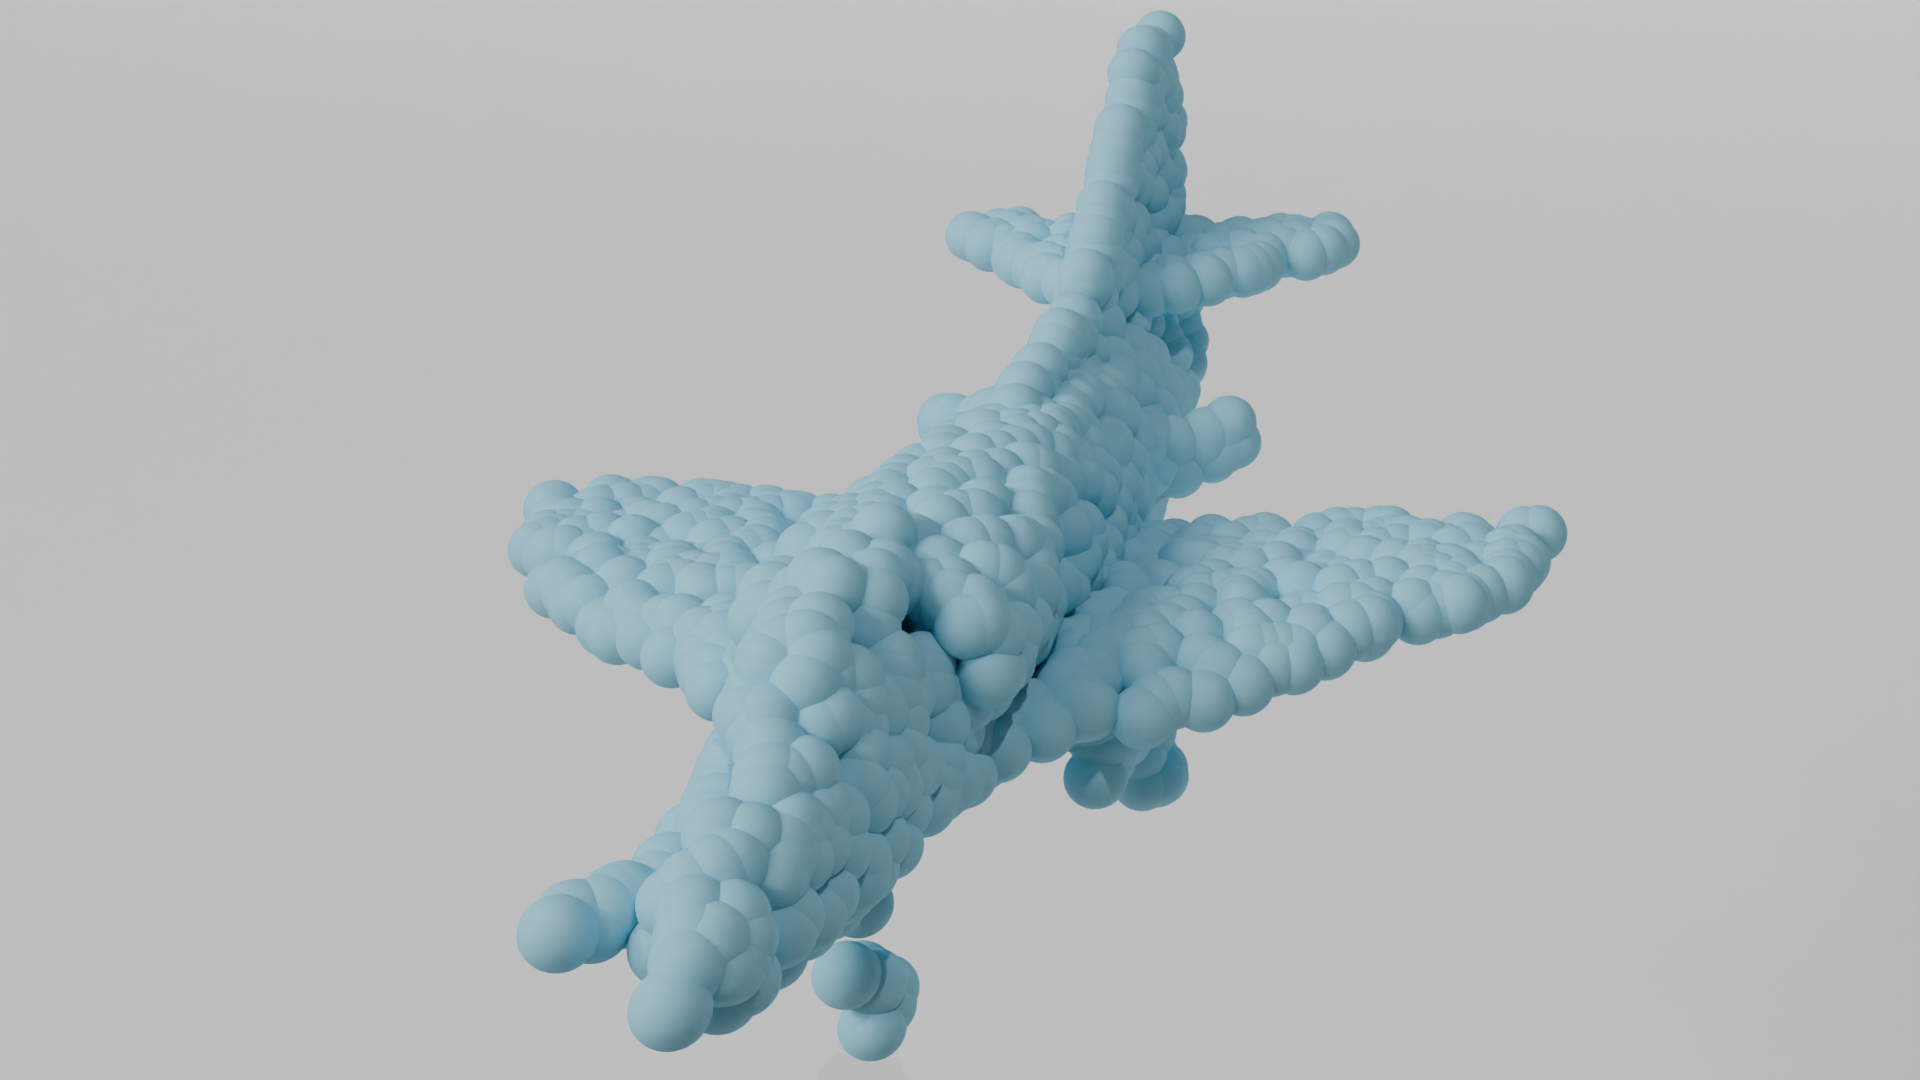
\includegraphics[width=\textwidth]{figures/com_ap3.png}
        \caption{Airplane 3}
    \end{subfigure}
    \caption{Grid test}
    \label{fig:airplane}
\end{figure}

\begin{figure}[htb]
      \centering
      \begin{subfigure}[t]{\dimexpr0.315\textwidth+20pt\relax}
        \makebox[20pt]{\raisebox{30pt}{\rotatebox[origin=c]{90}{\small Input}}}%
        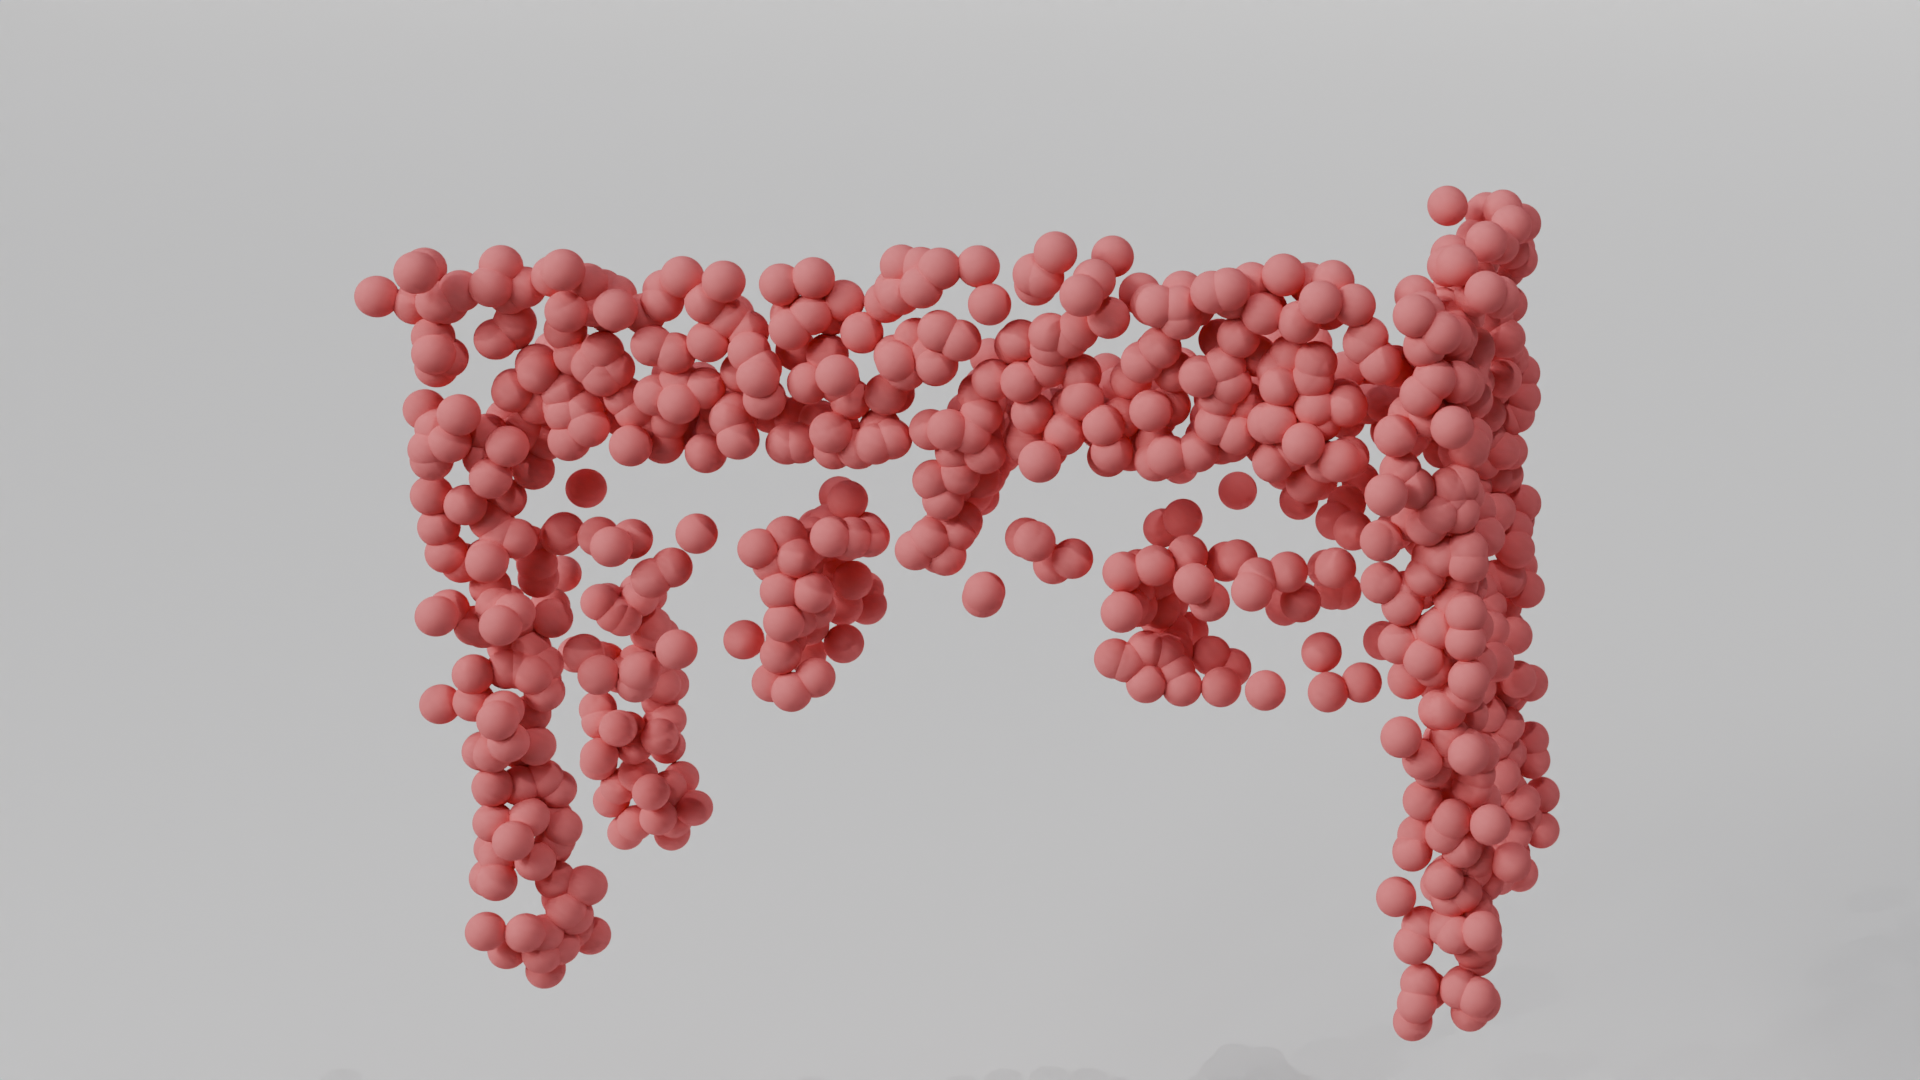
\includegraphics[width=\dimexpr\linewidth-20pt\relax]{figures/part_t1.png}
        \makebox[20pt]{\raisebox{30pt}{\rotatebox[origin=c]{90}{\small DropCon}}}%
        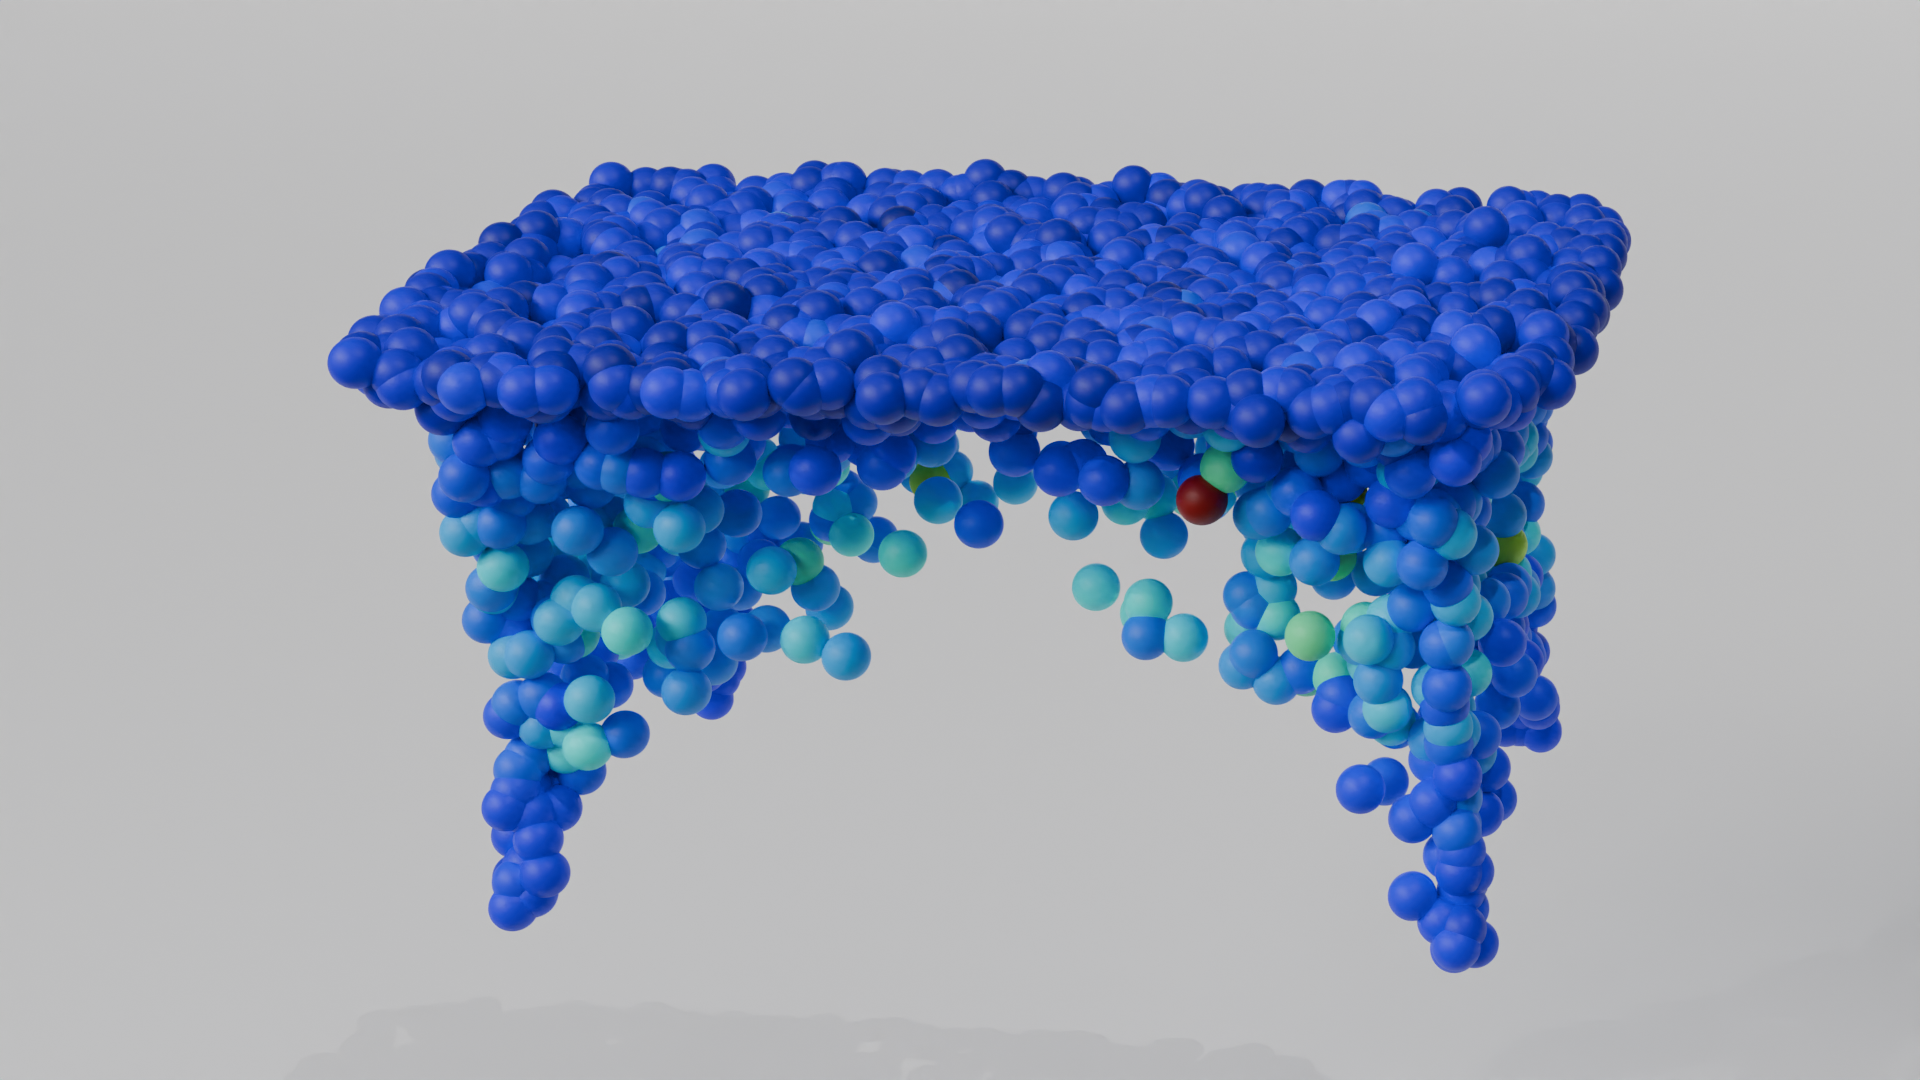
\includegraphics[width=\dimexpr\linewidth-20pt\relax]{figures/dc_lin_t1.png}
        \makebox[20pt]{\raisebox{30pt}{\rotatebox[origin=c]{90}{\small Dropout}}}%
        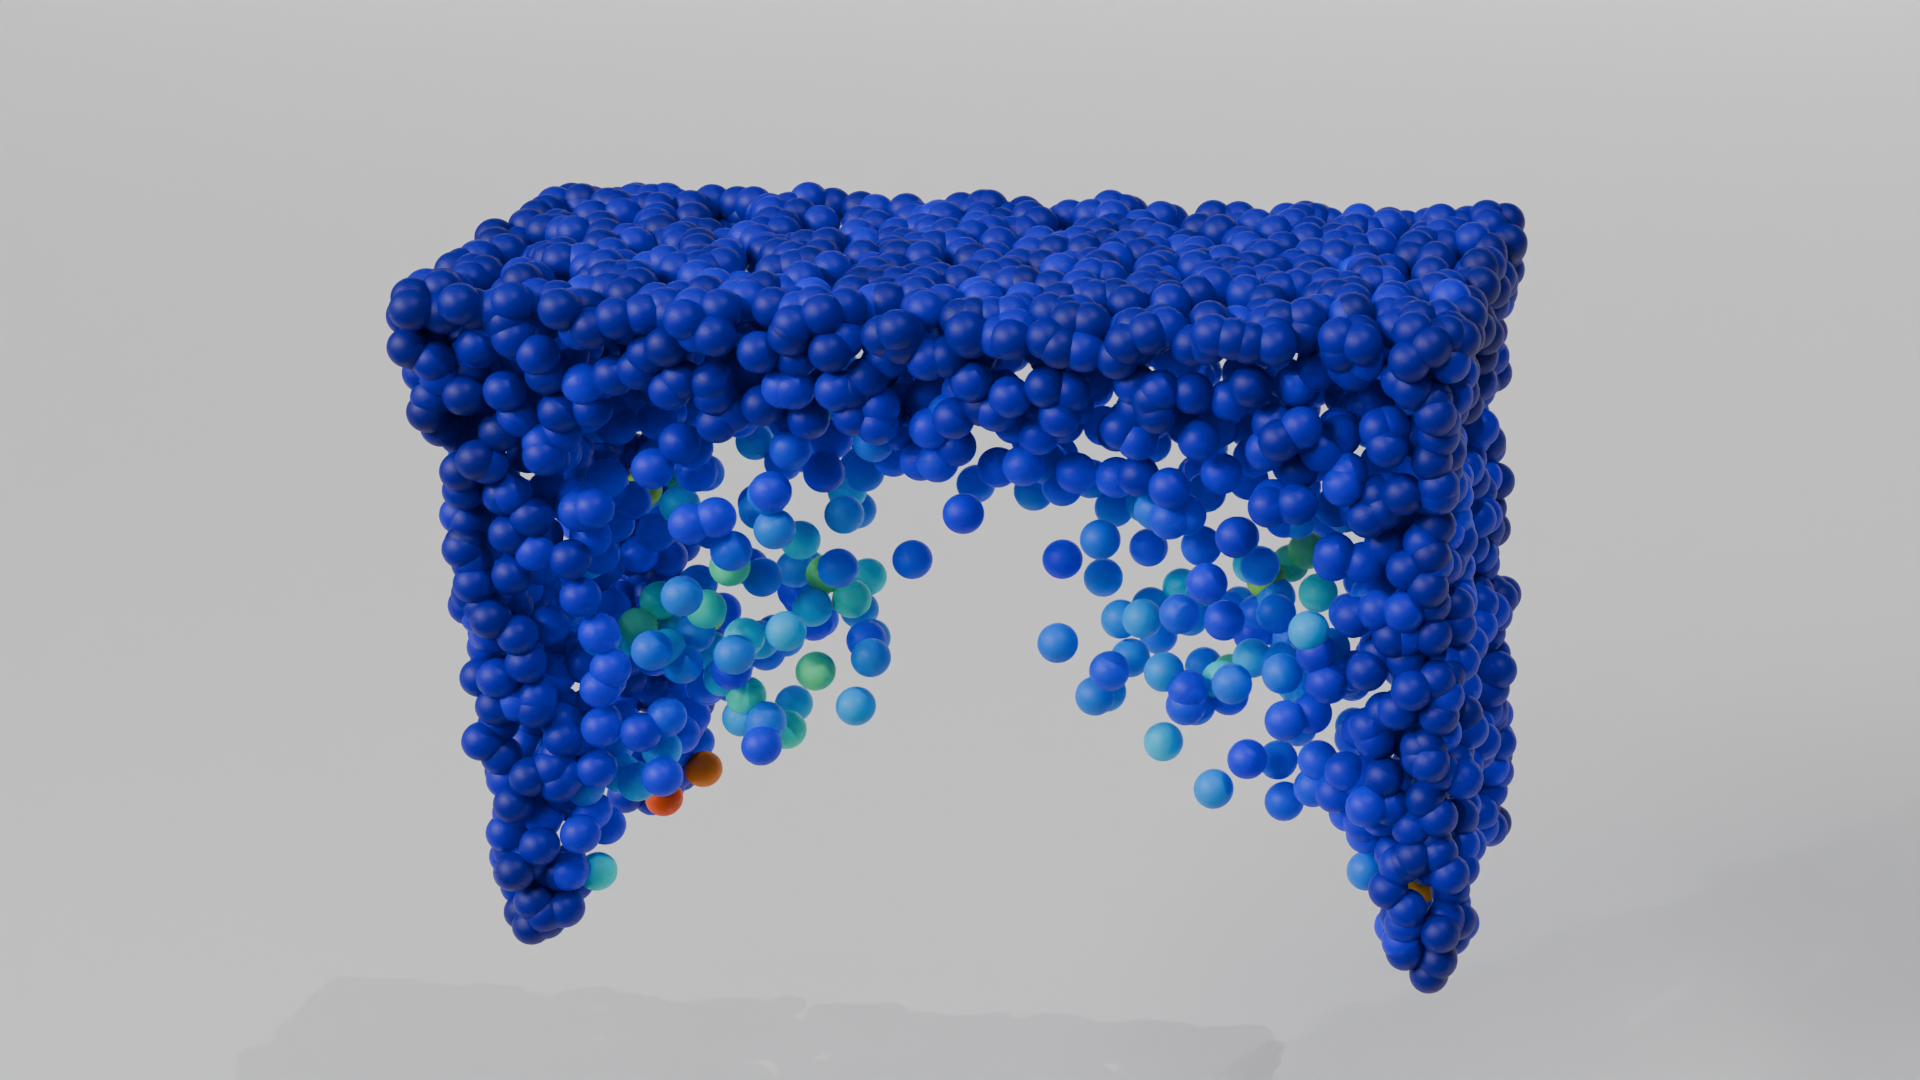
\includegraphics[width=\dimexpr\linewidth-20pt\relax]{figures/do_lin_t1.png}
        \makebox[20pt]{\raisebox{30pt}{\rotatebox[origin=c]{90}{\small Ensemble}}}%
        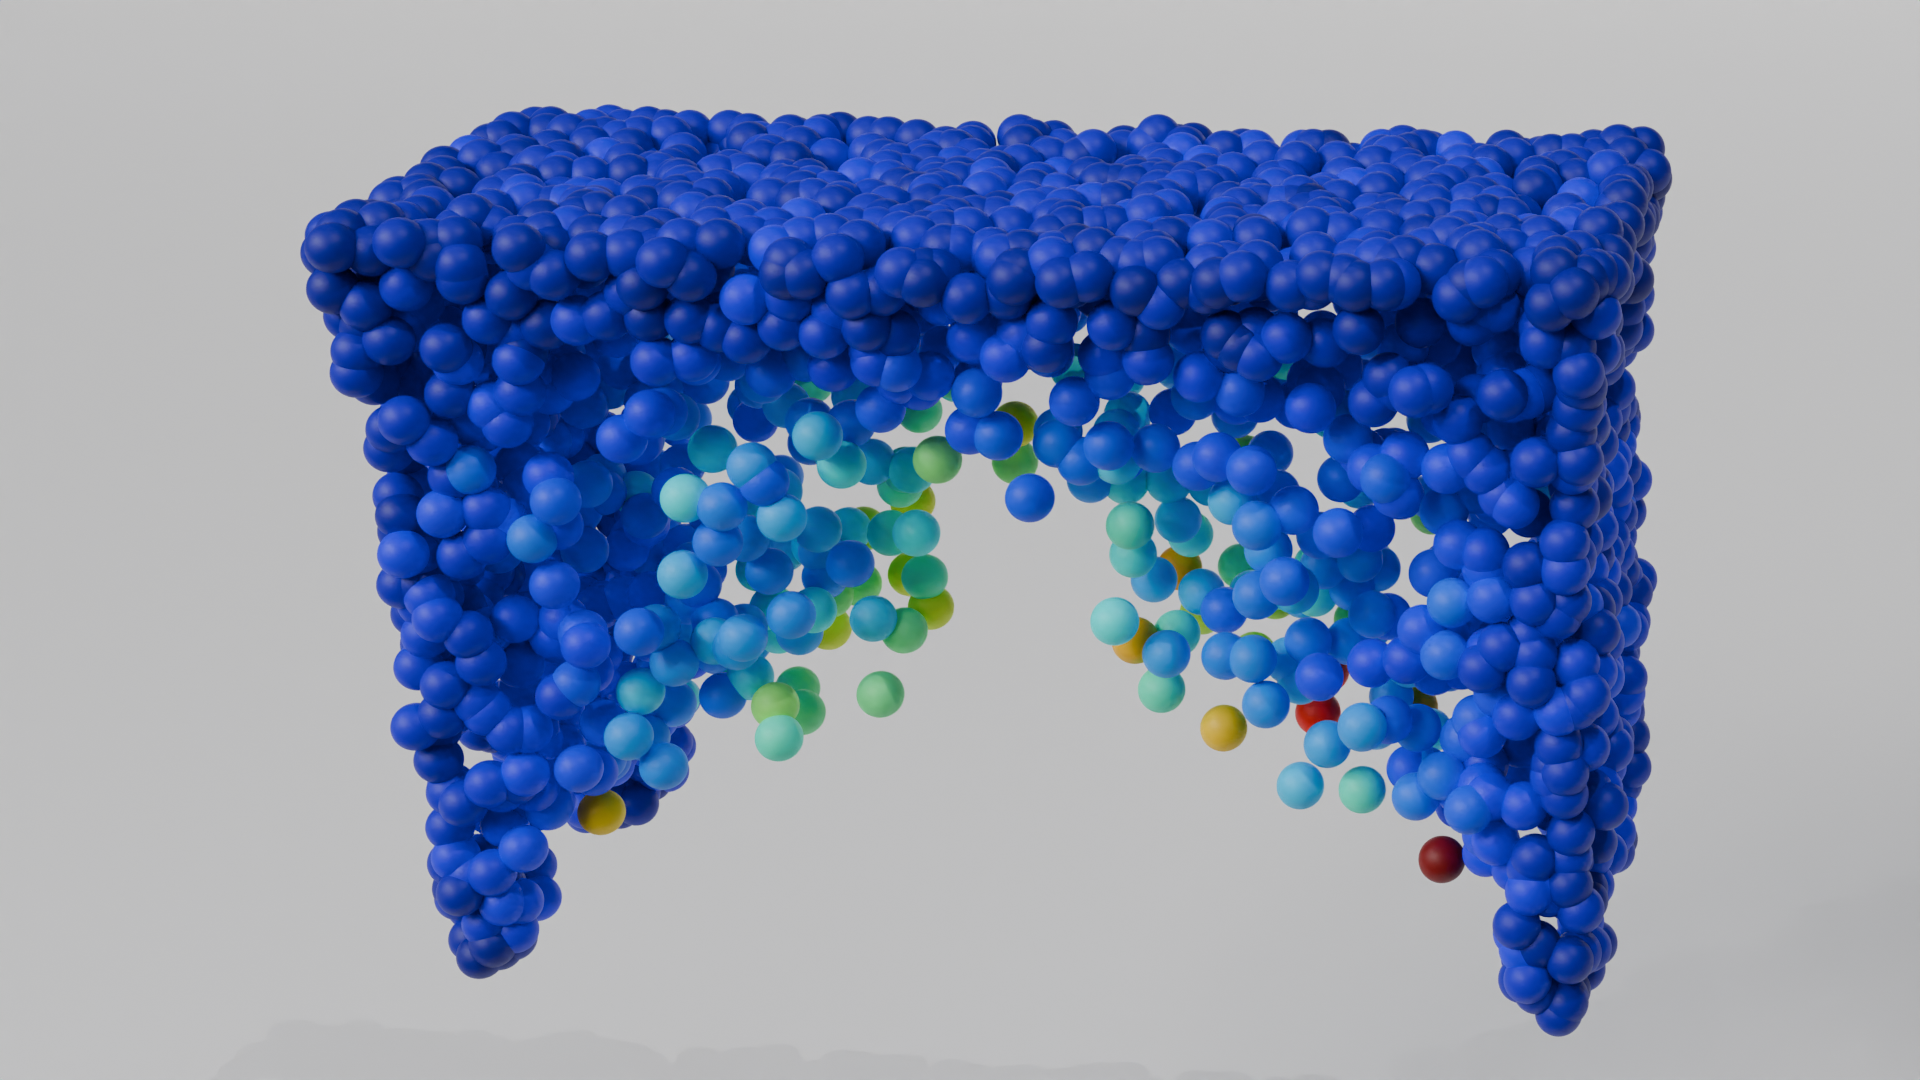
\includegraphics[width=\dimexpr\linewidth-20pt\relax]{figures/ens_lin_t1.png}
        \makebox[20pt]{\raisebox{30pt}{\rotatebox[origin=c]{90}{\small Implicit}}}%
        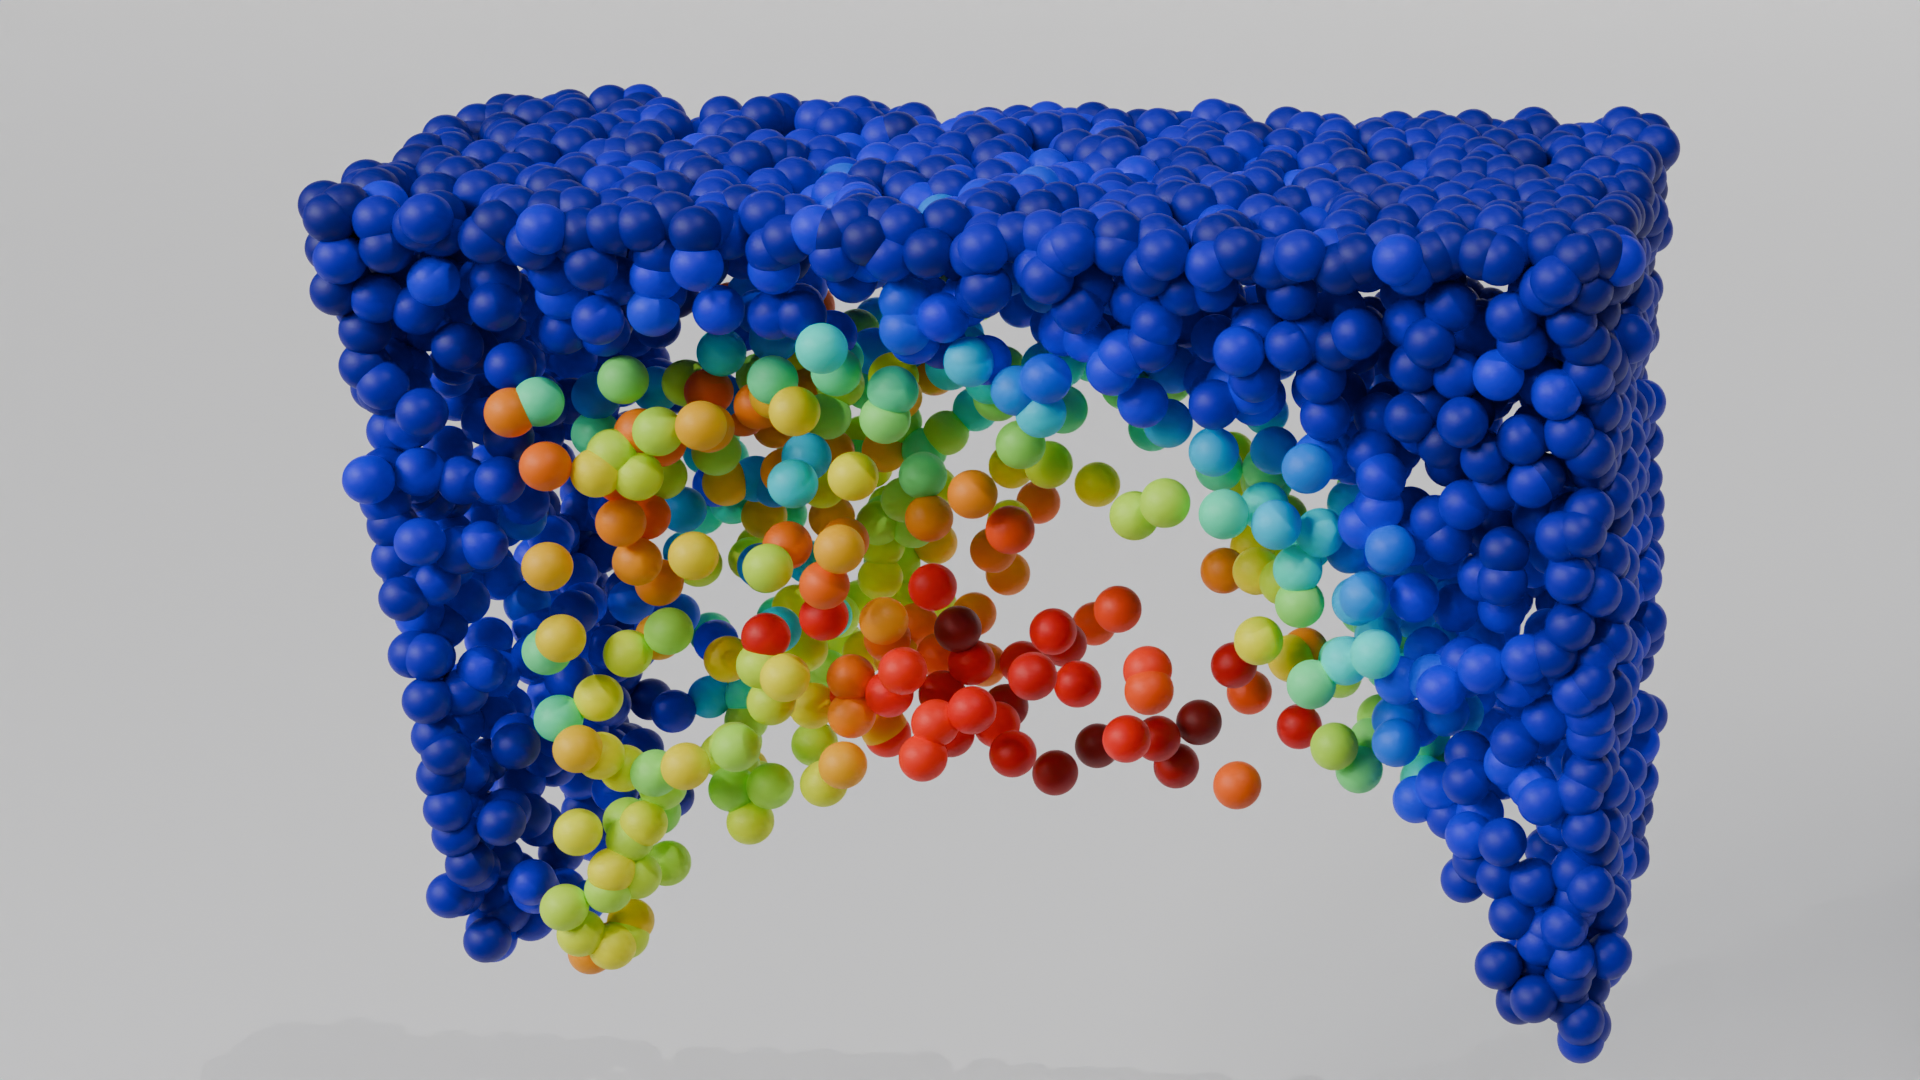
\includegraphics[width=\dimexpr\linewidth-20pt\relax]{figures/iml_lin_t1.png}
        \makebox[20pt]{\raisebox{30pt}{\rotatebox[origin=c]{90}{\small GT}}}%
        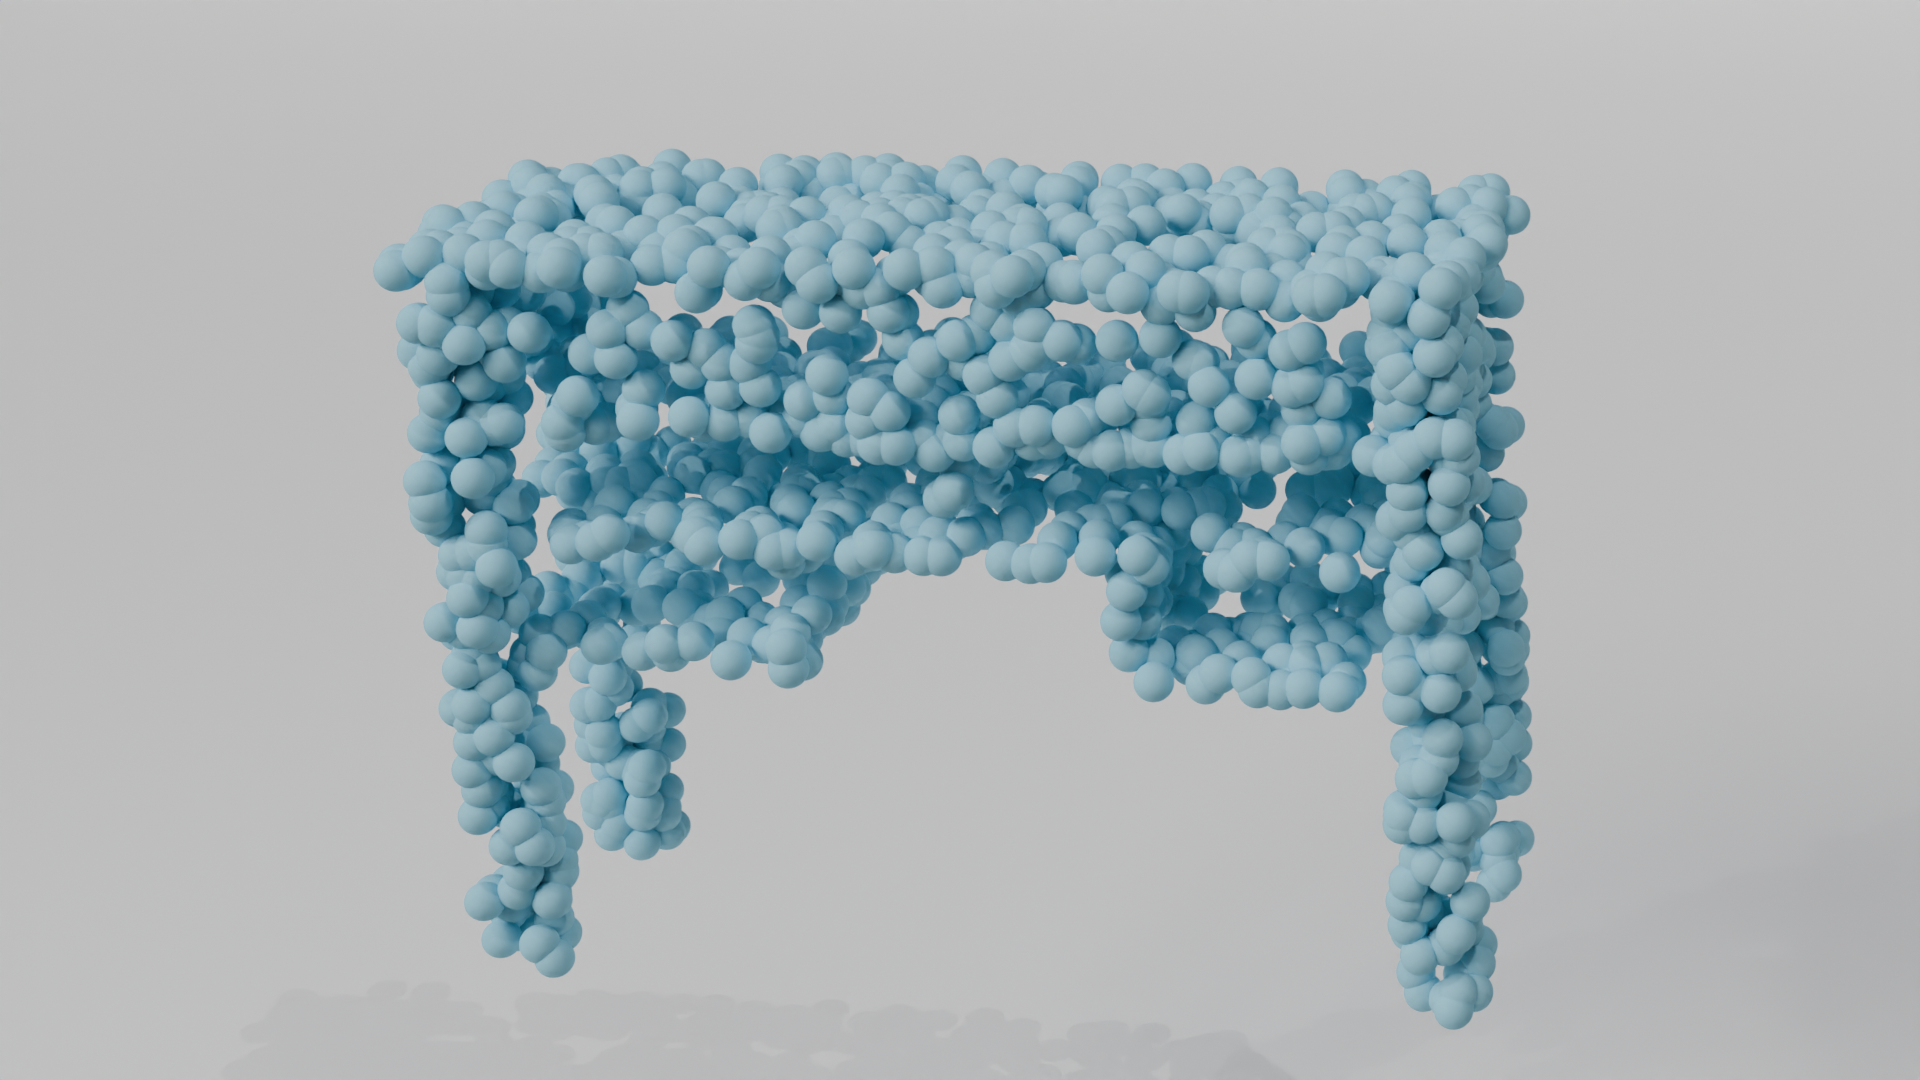
\includegraphics[width=\dimexpr\linewidth-20pt\relax]{figures/com_t1.png}
        \caption{Table 1}
    \end{subfigure}\hfill
    \begin{subfigure}[t]{0.315\textwidth}
        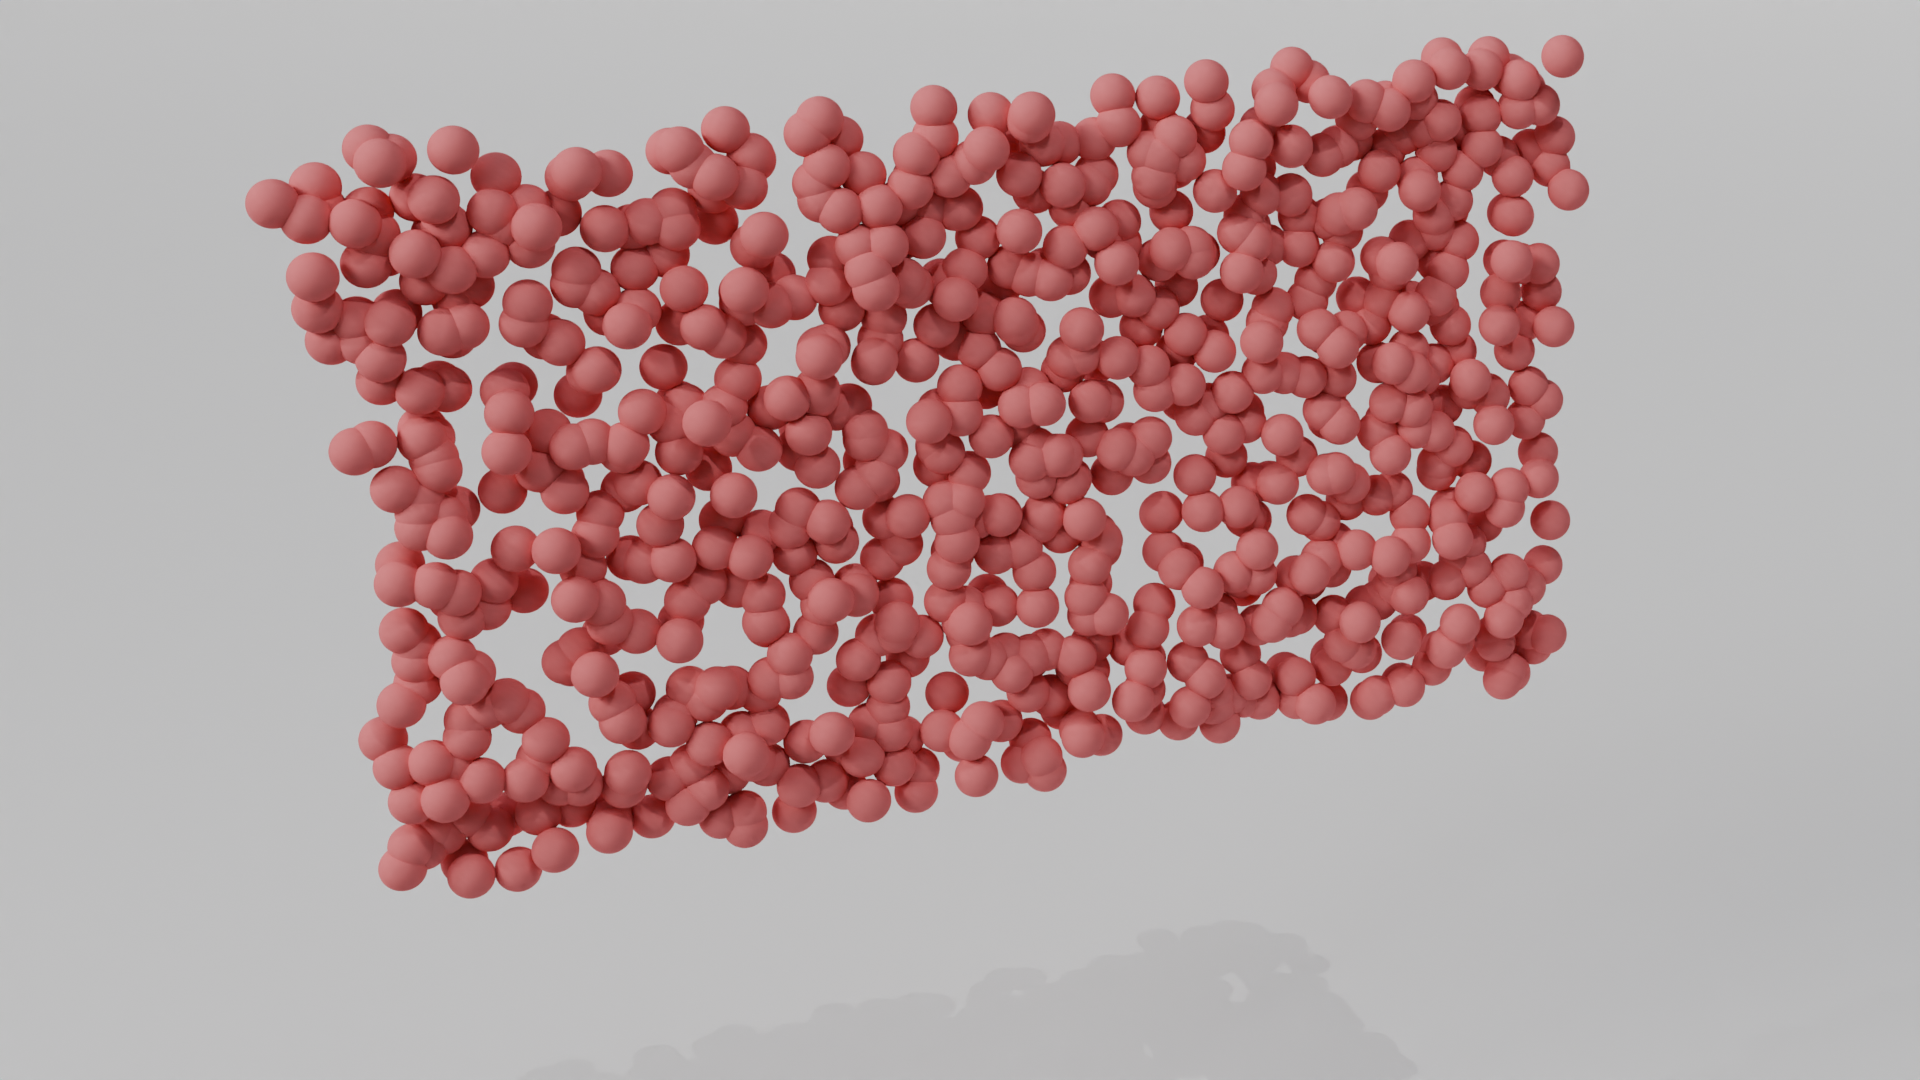
\includegraphics[width=\textwidth]{figures/part_t2.png}
        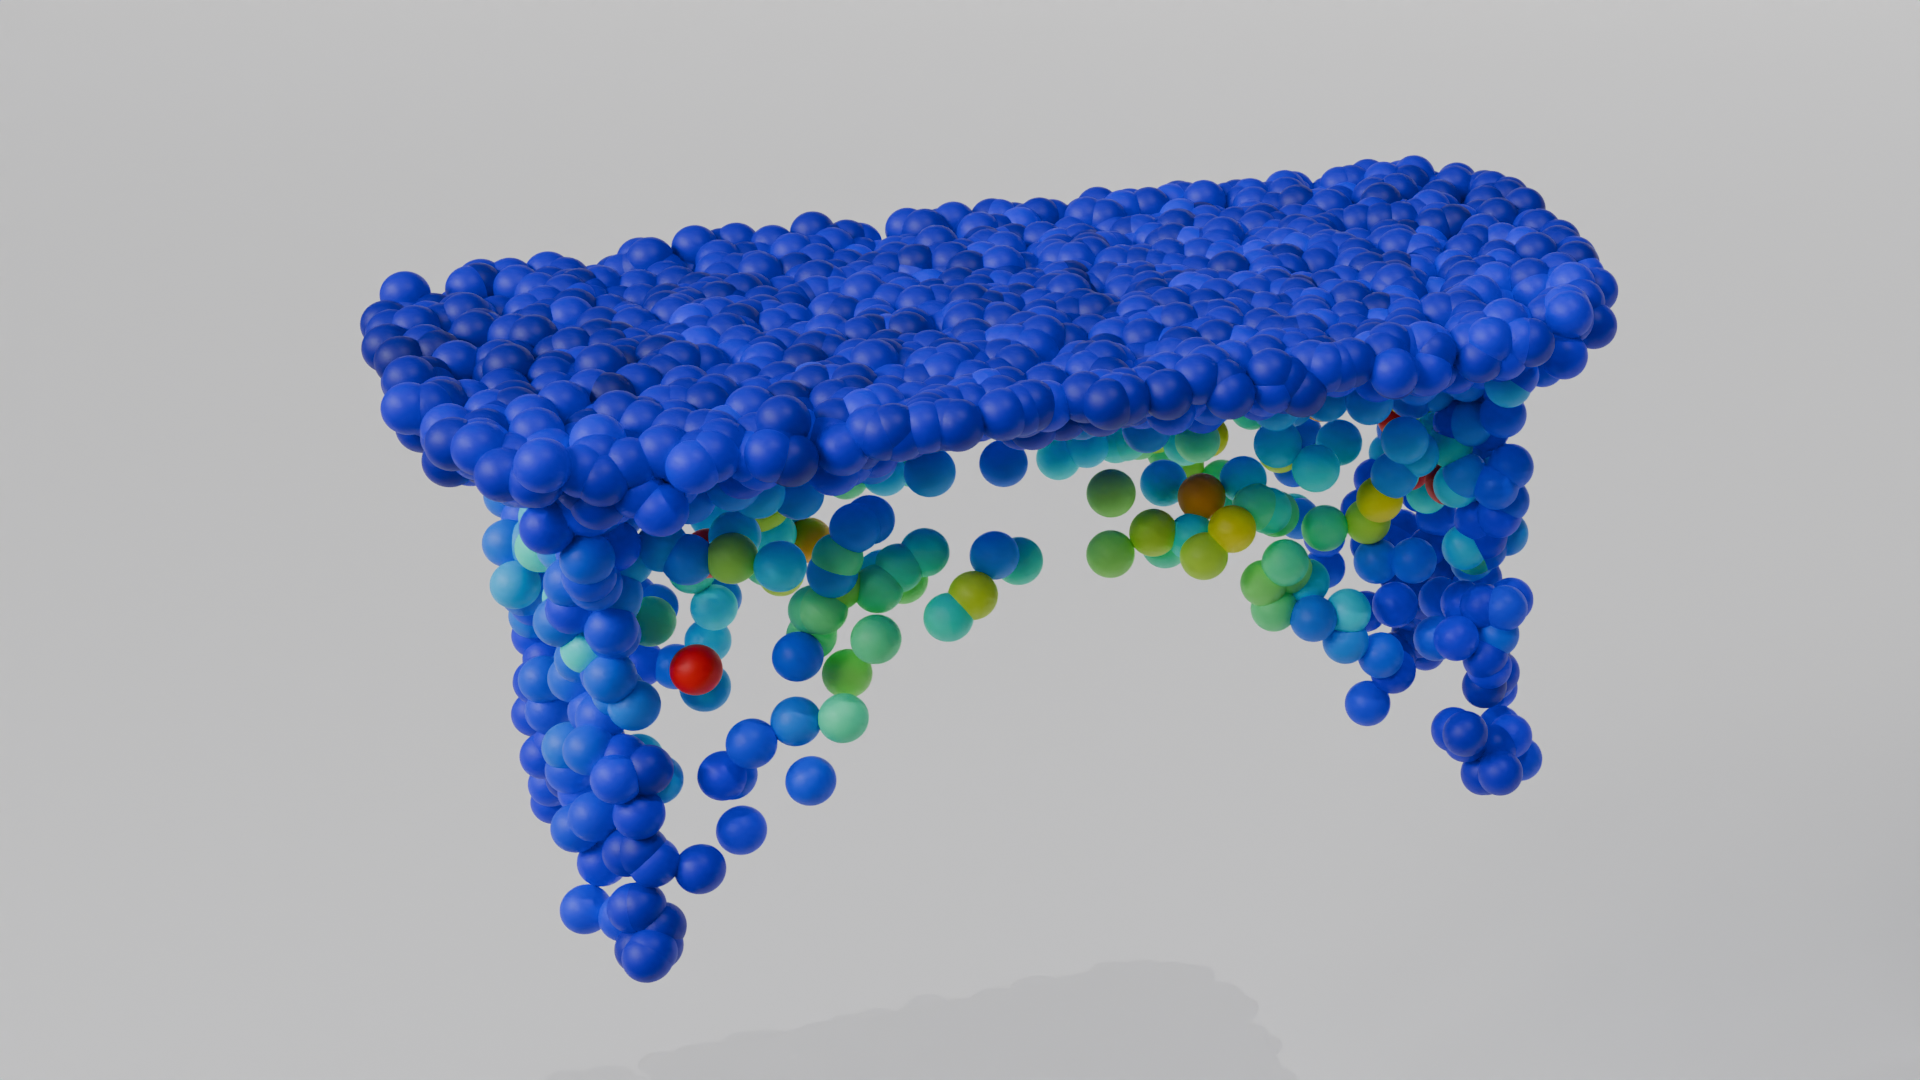
\includegraphics[width=\textwidth]{figures/dc_lin_t2.png}
        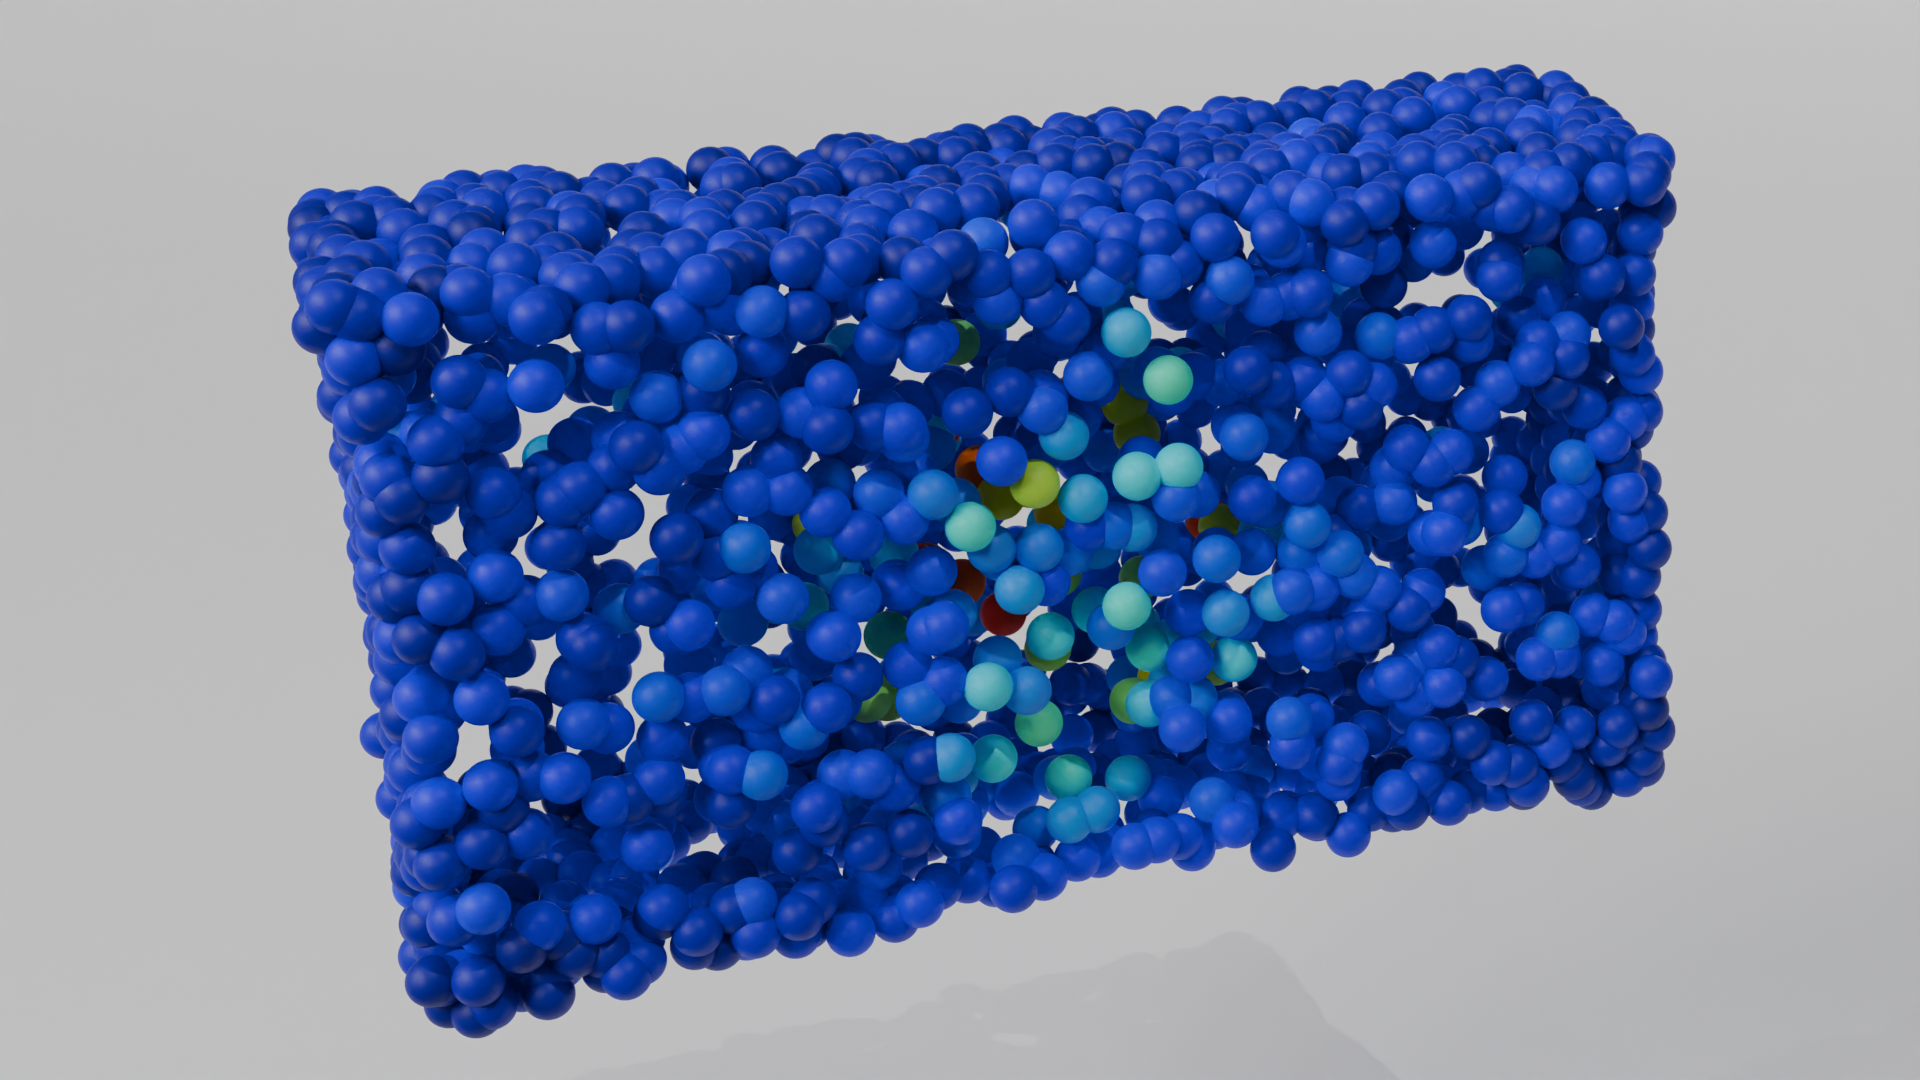
\includegraphics[width=\textwidth]{figures/do_lin_t2.png}
        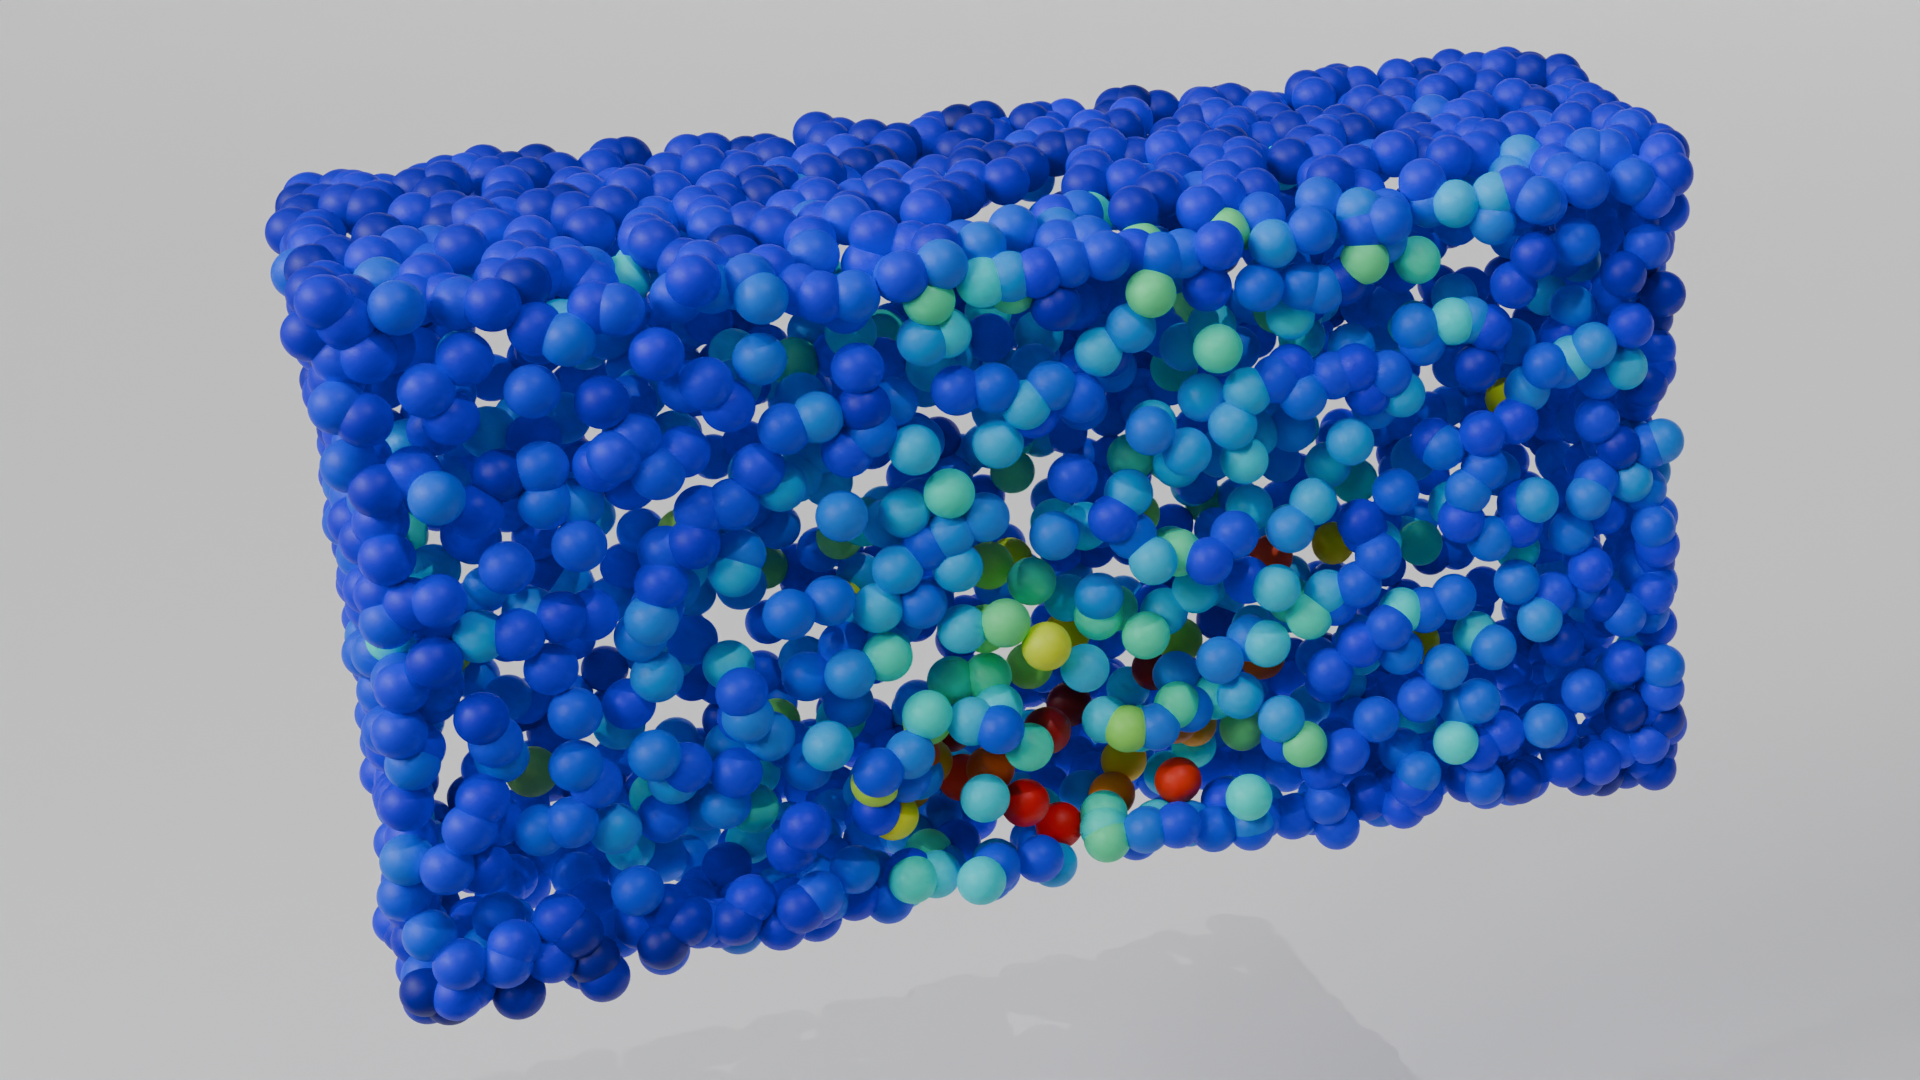
\includegraphics[width=\textwidth]{figures/ens_lin_t2.png}
        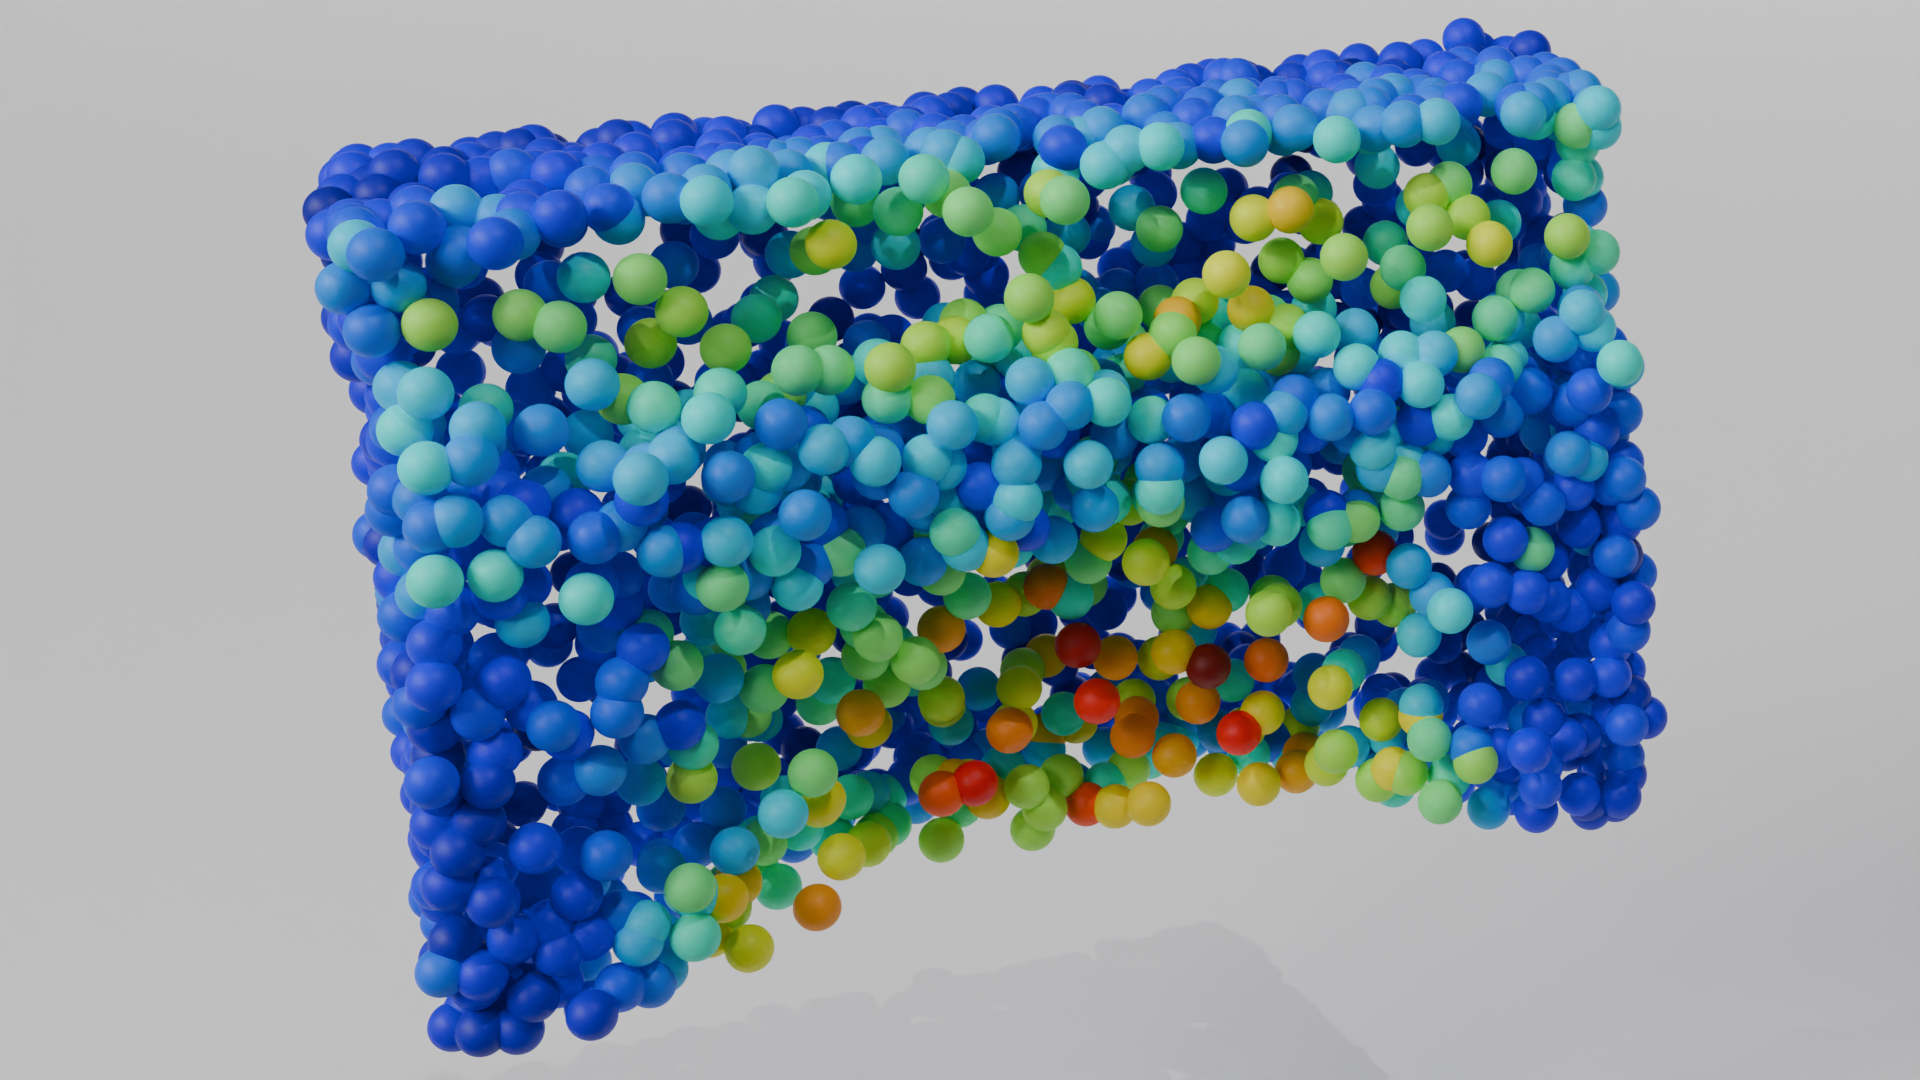
\includegraphics[width=\textwidth]{figures/iml_lin_t2.png}
        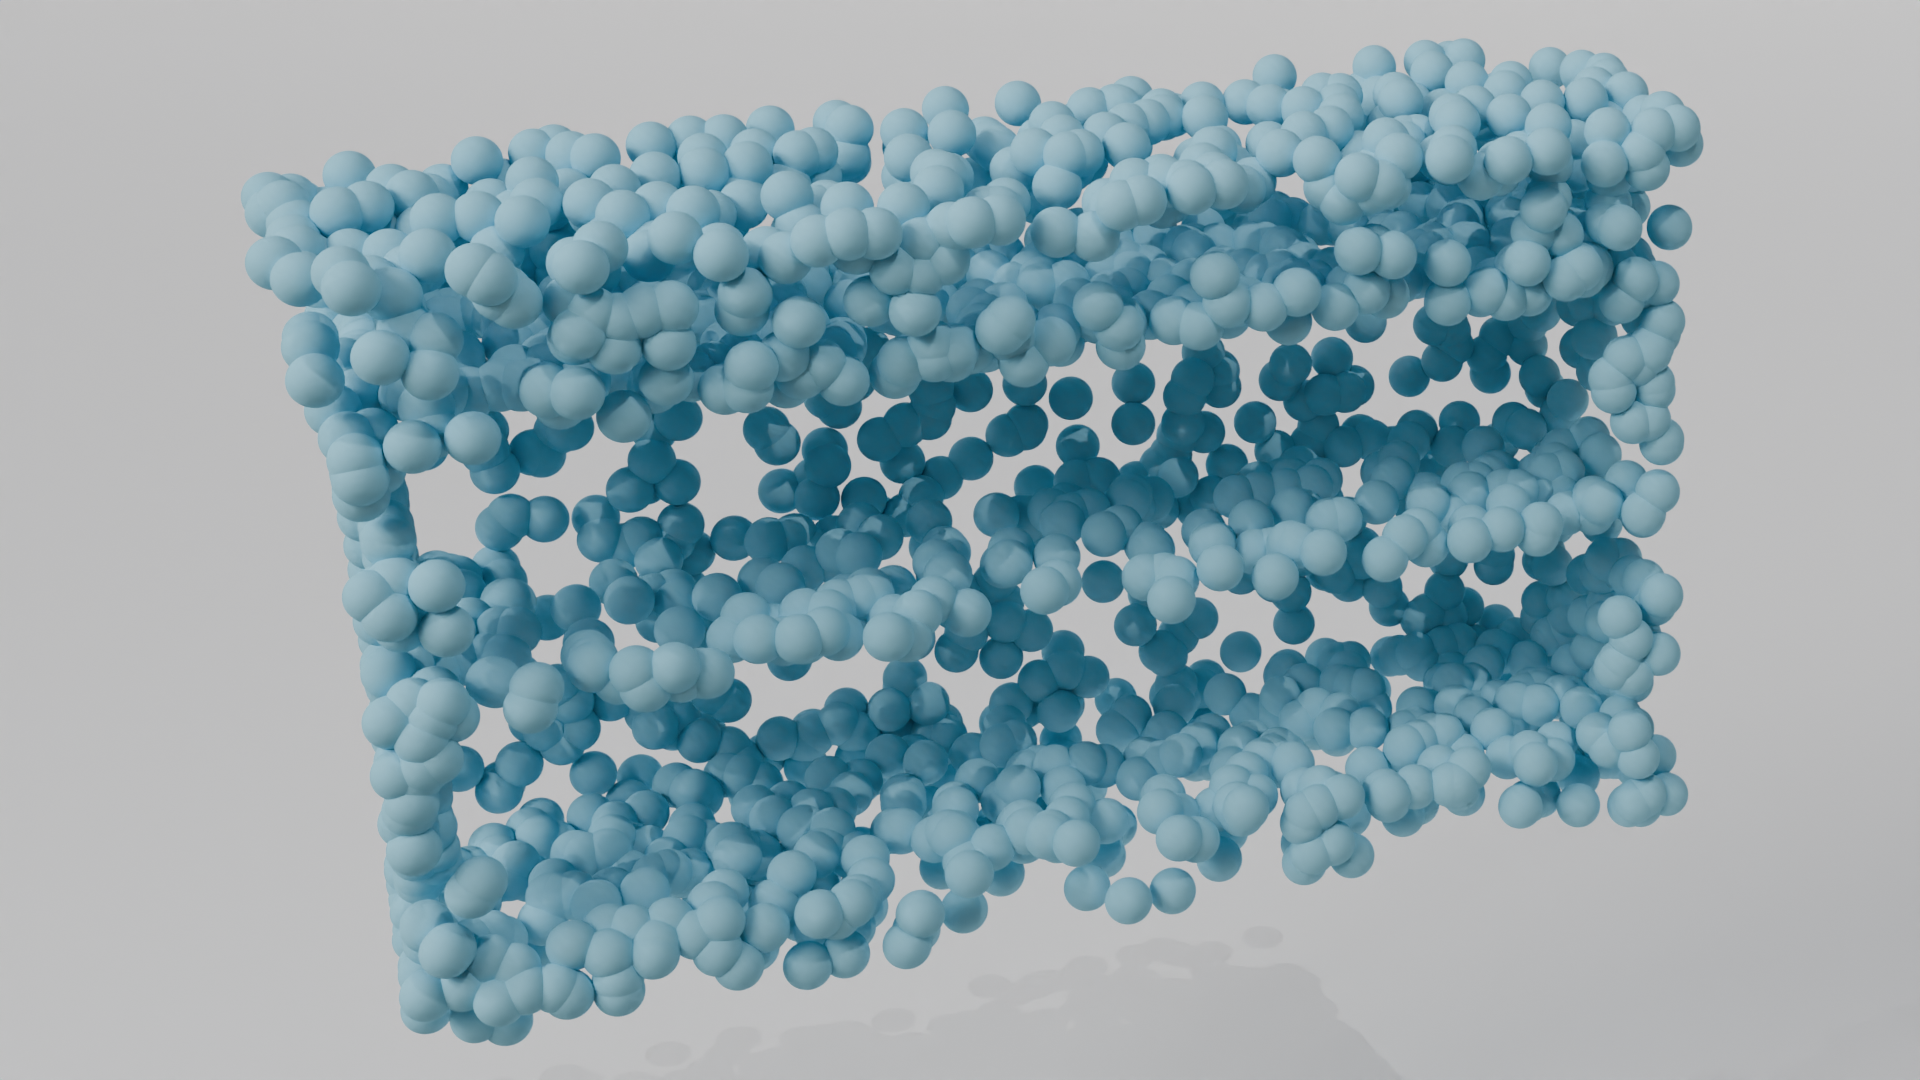
\includegraphics[width=\textwidth]{figures/com_t2.png}
        \caption{Table 2}
    \end{subfigure}\hfill
    \begin{subfigure}[t]{0.315\textwidth}
        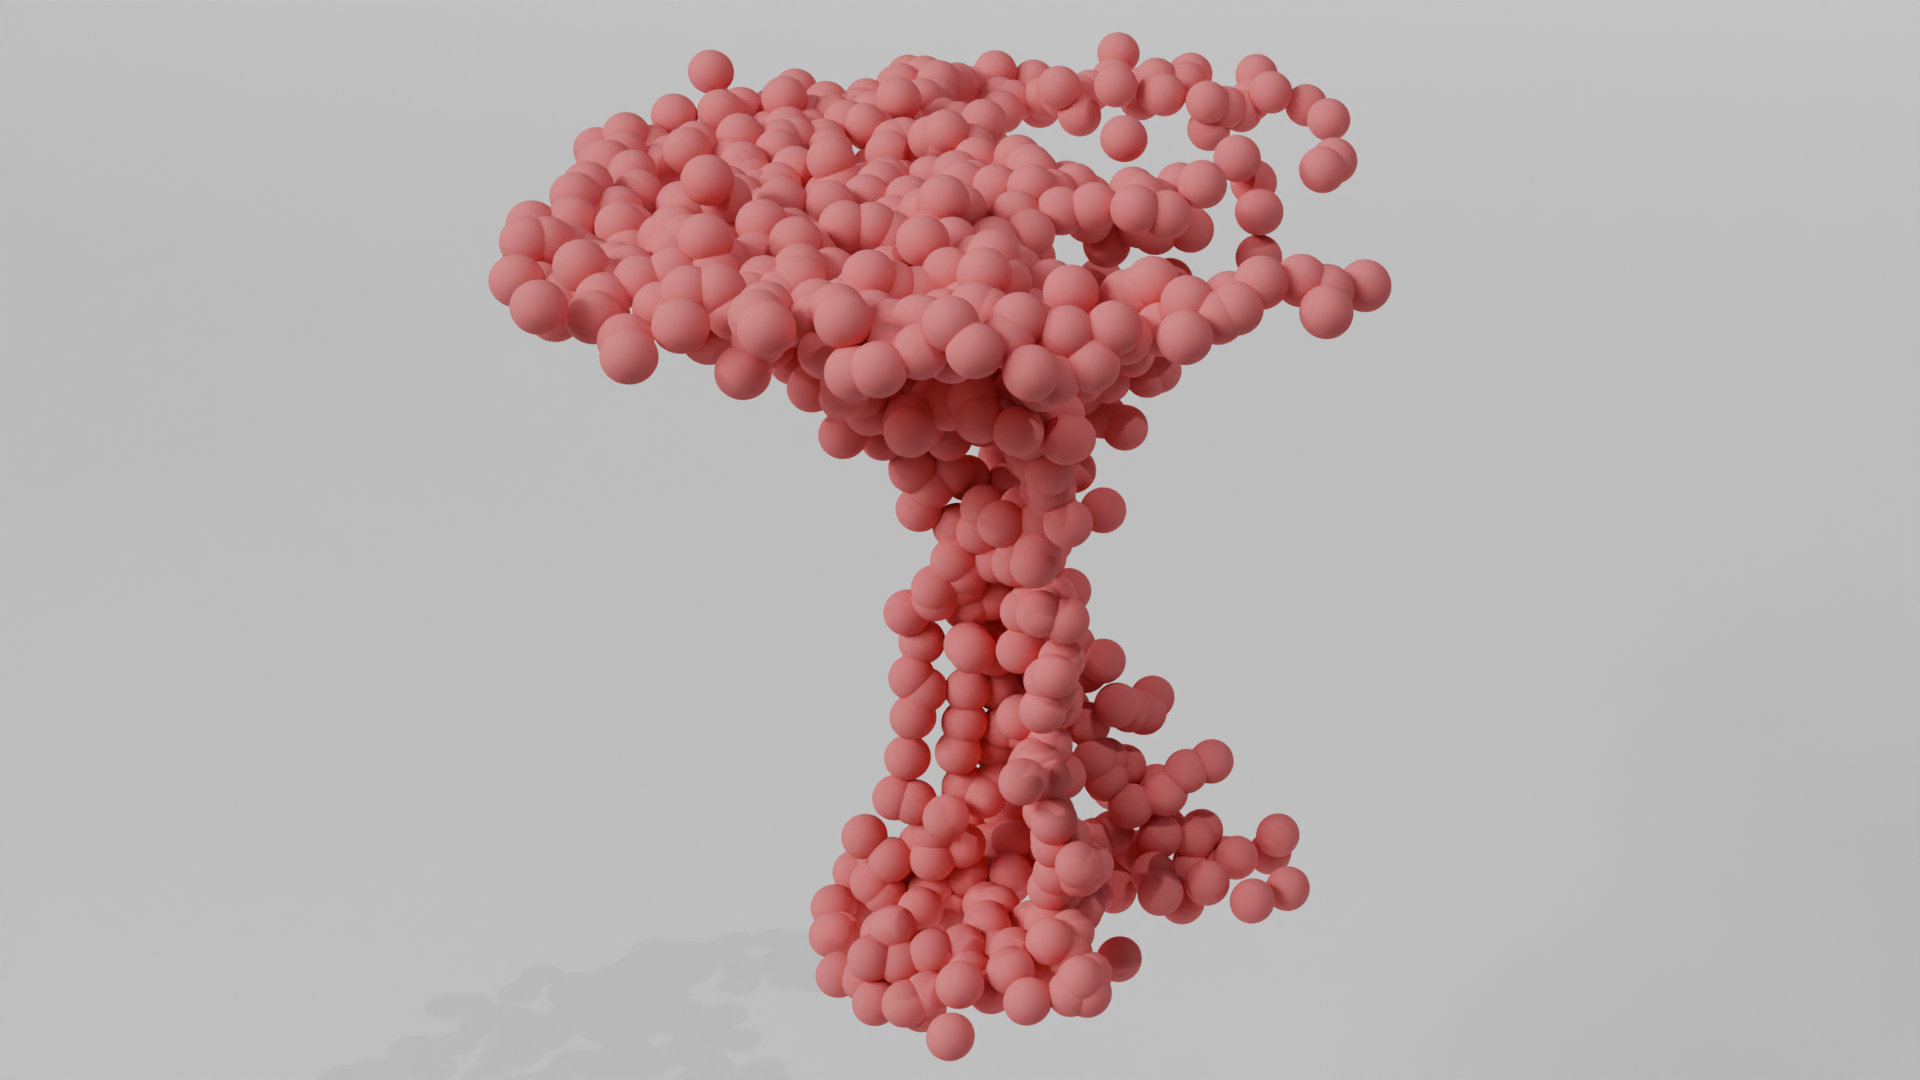
\includegraphics[width=\textwidth]{figures/part_t3.png}
        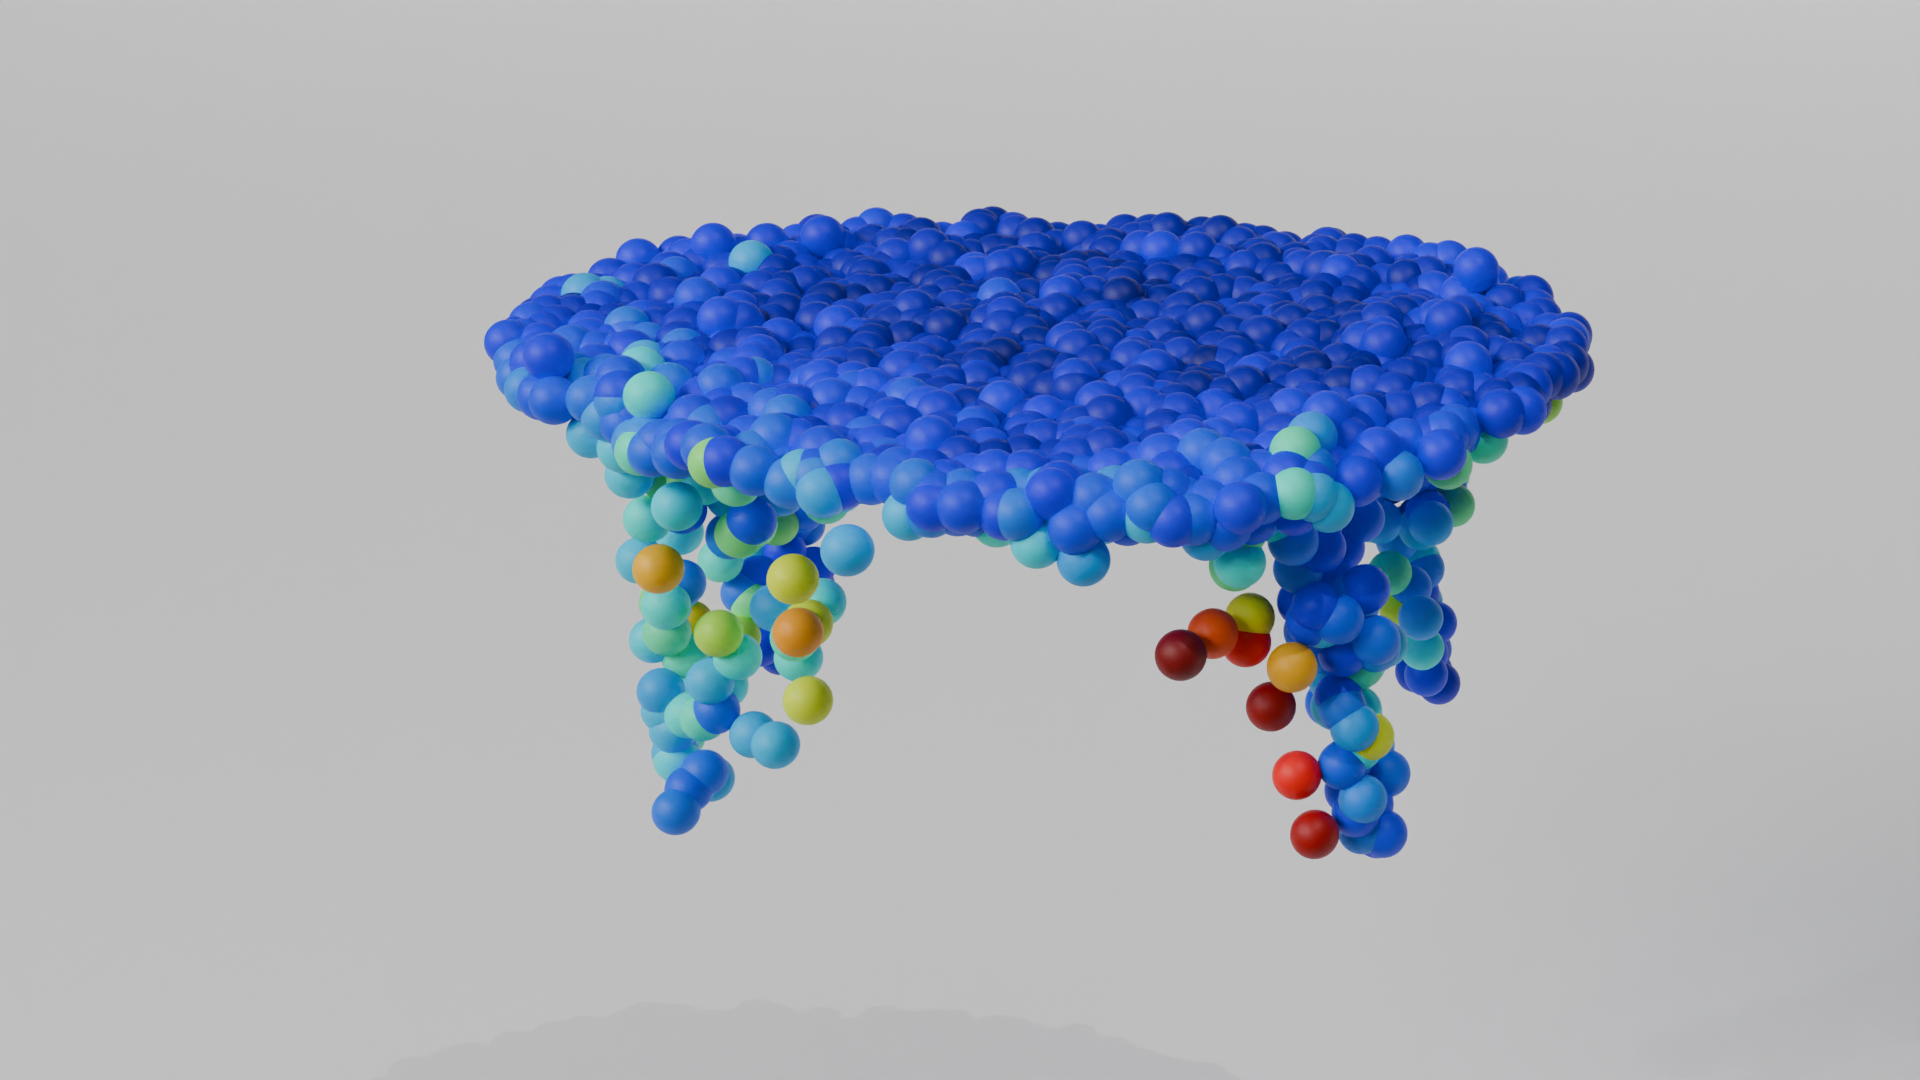
\includegraphics[width=\textwidth]{figures/dc_lin_t3.png}
        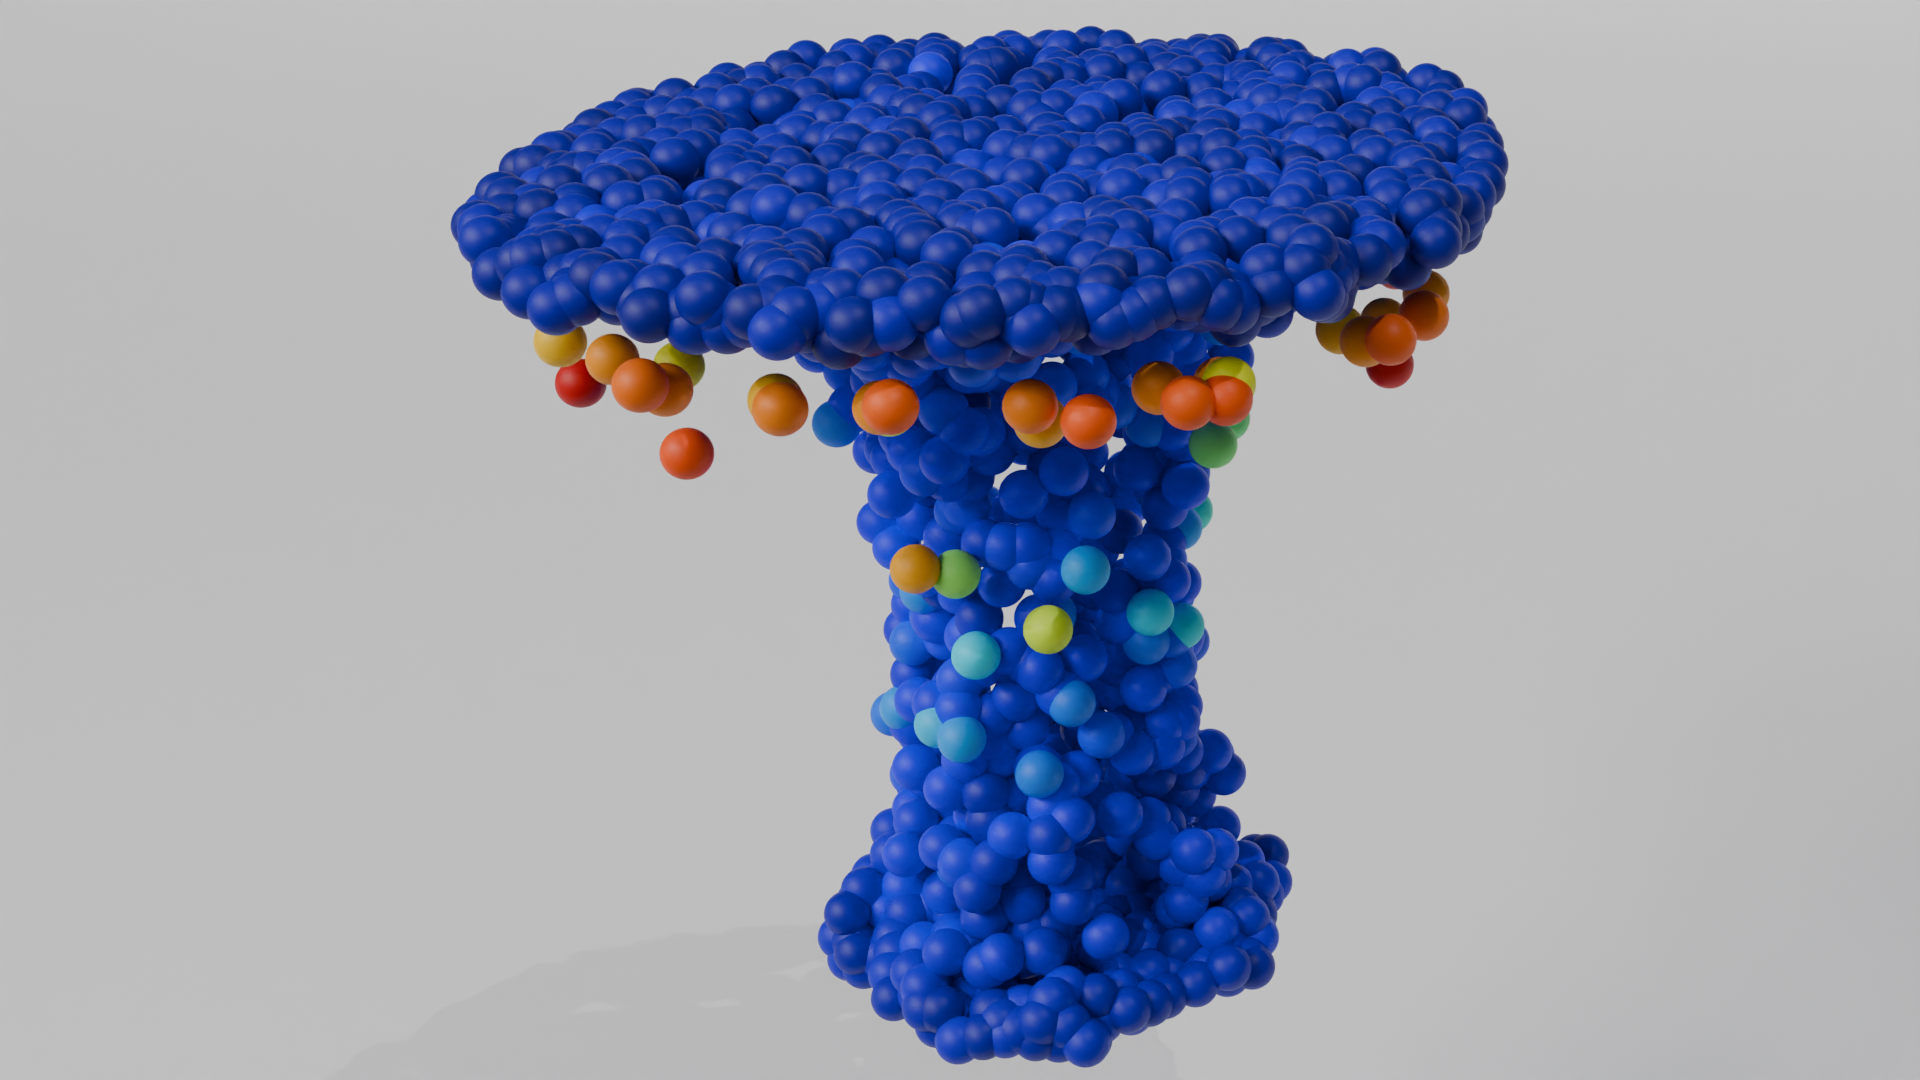
\includegraphics[width=\textwidth]{figures/do_lin_t3.png}
        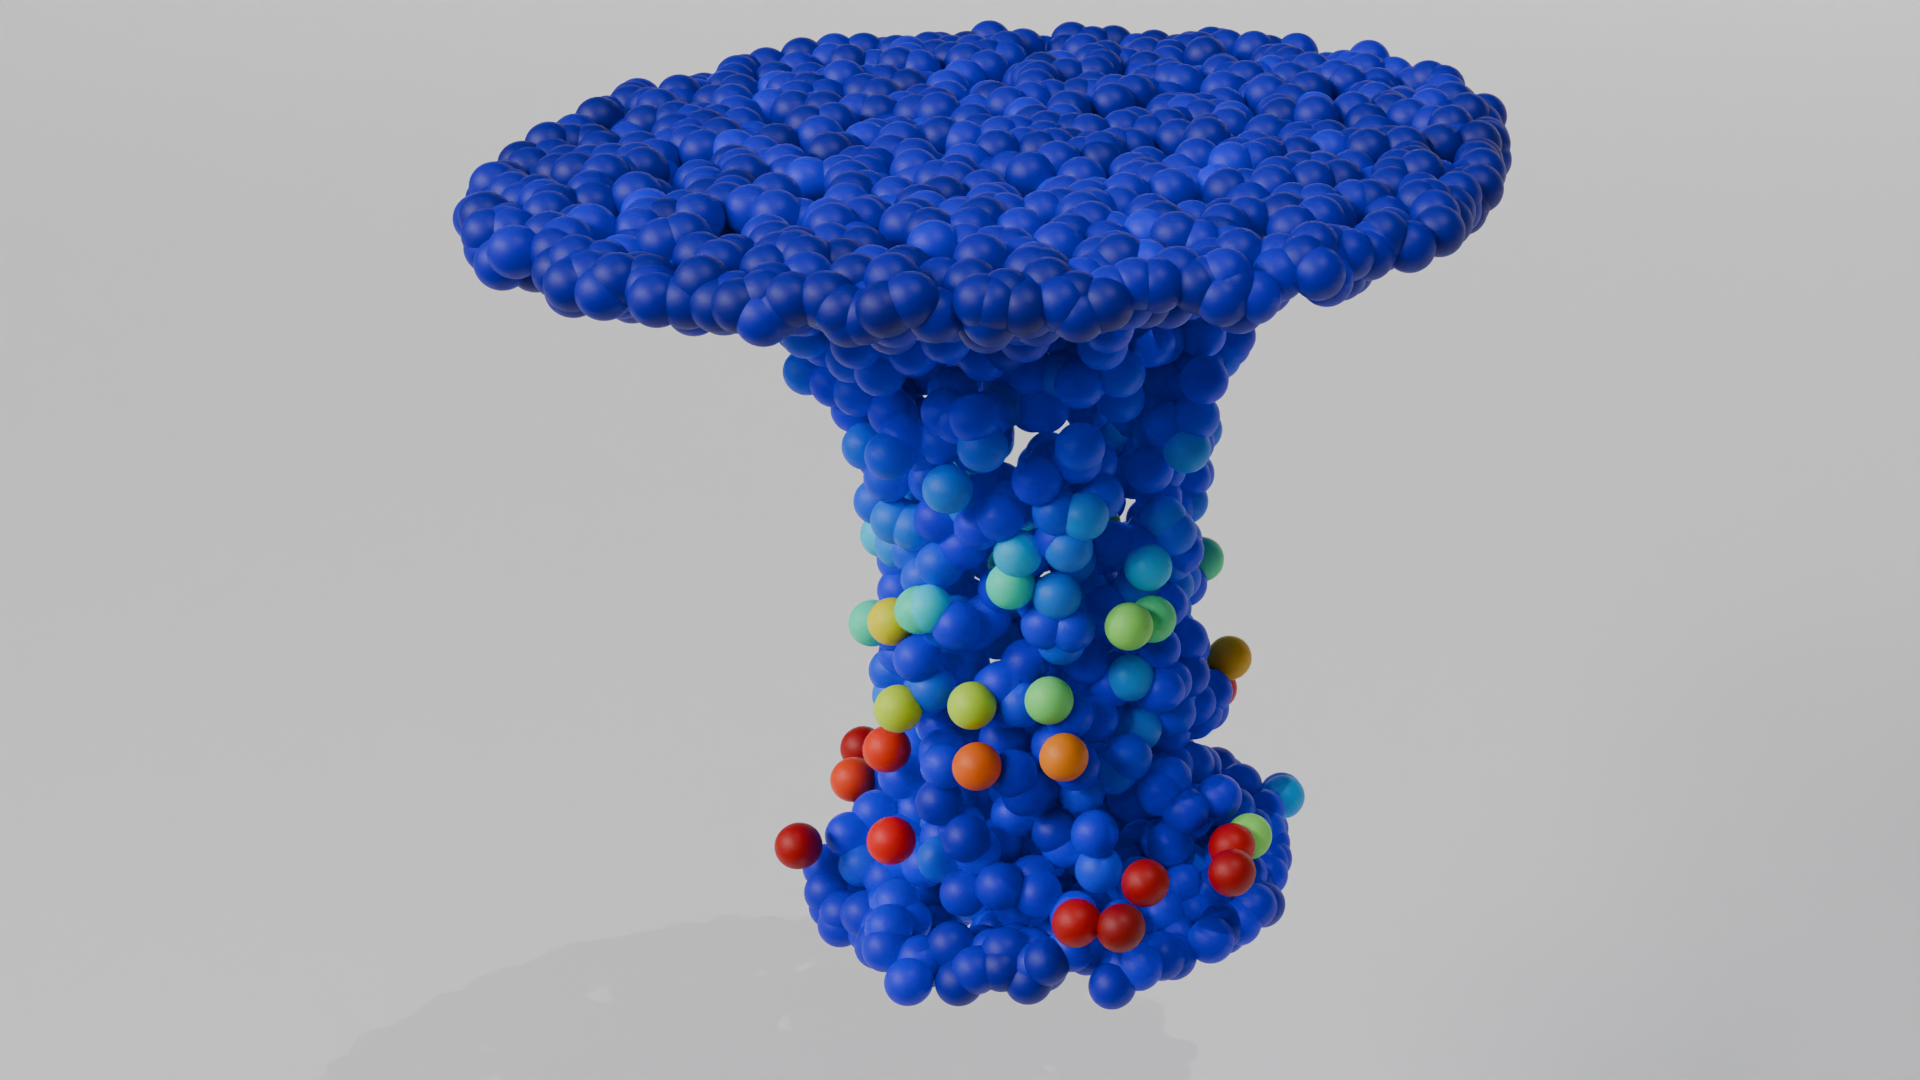
\includegraphics[width=\textwidth]{figures/ens_lin_t3.png}
        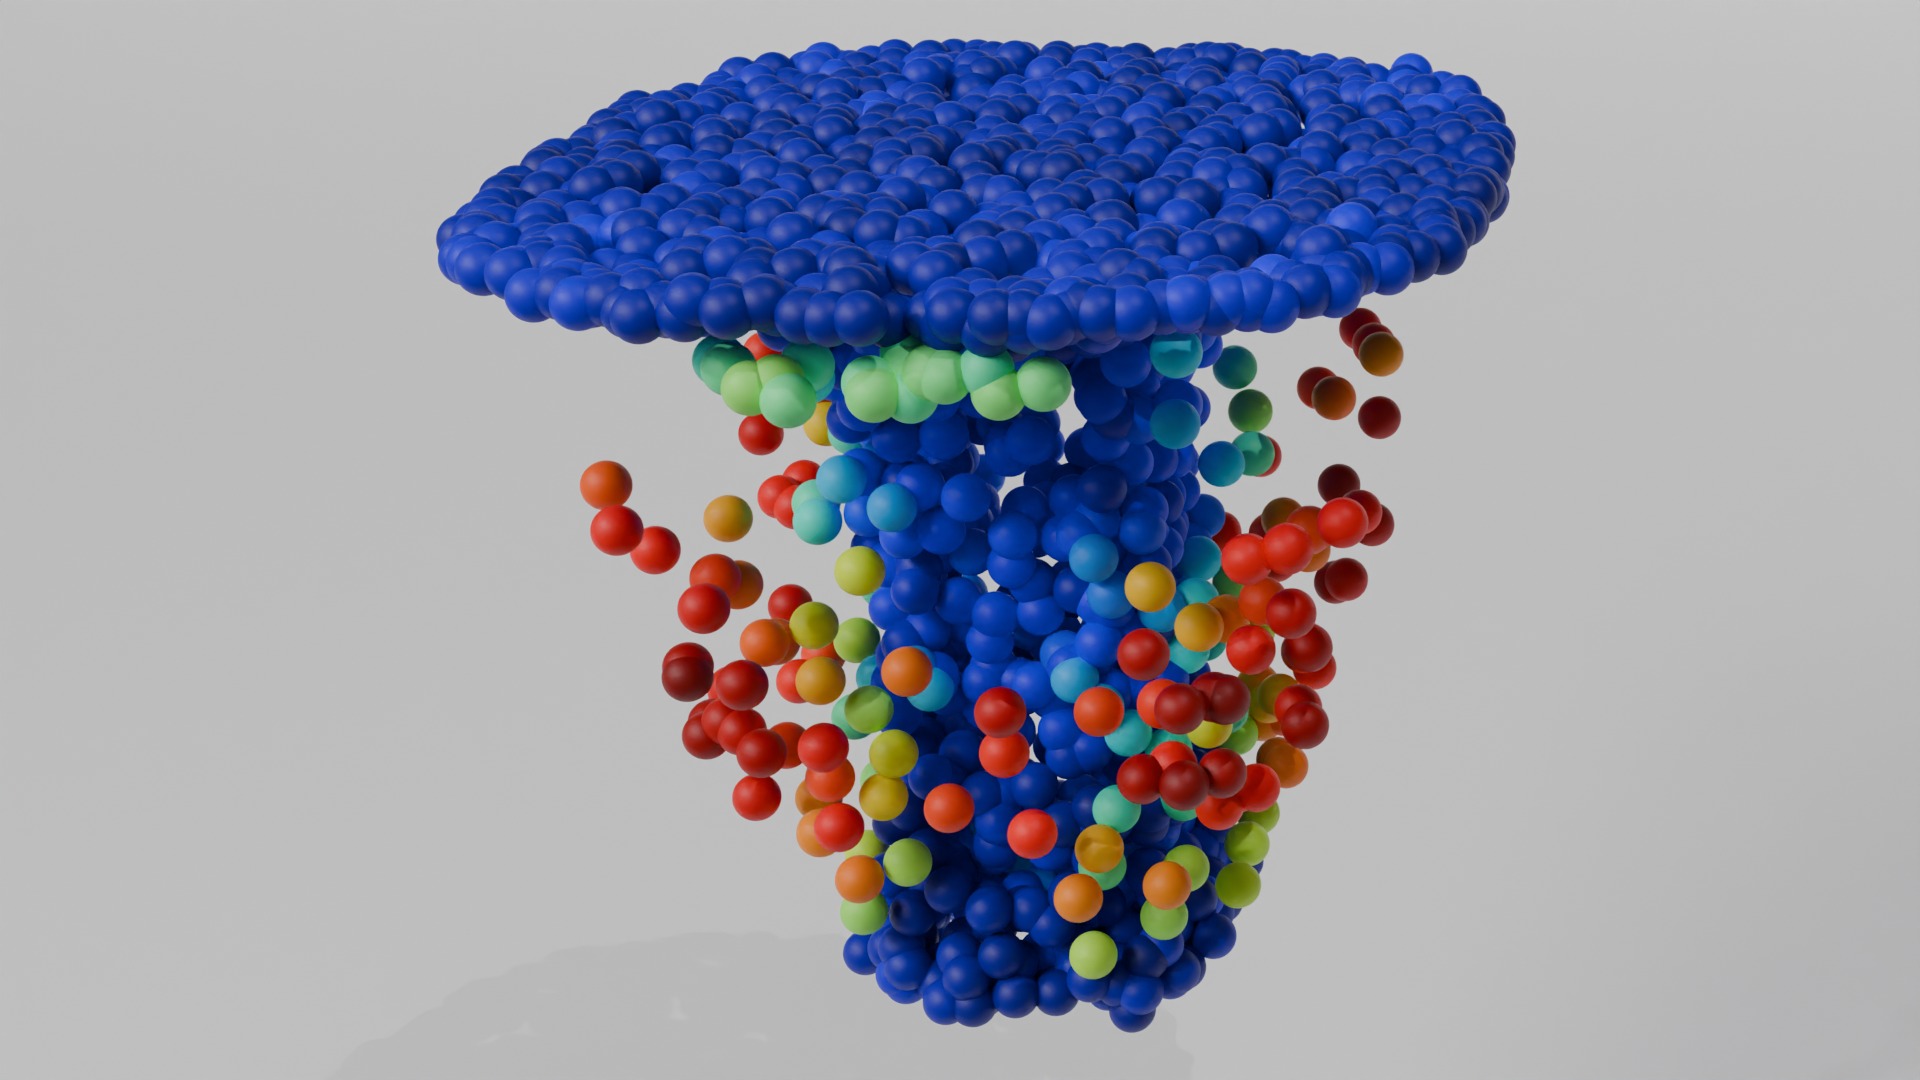
\includegraphics[width=\textwidth]{figures/iml_lin_t3.png}
        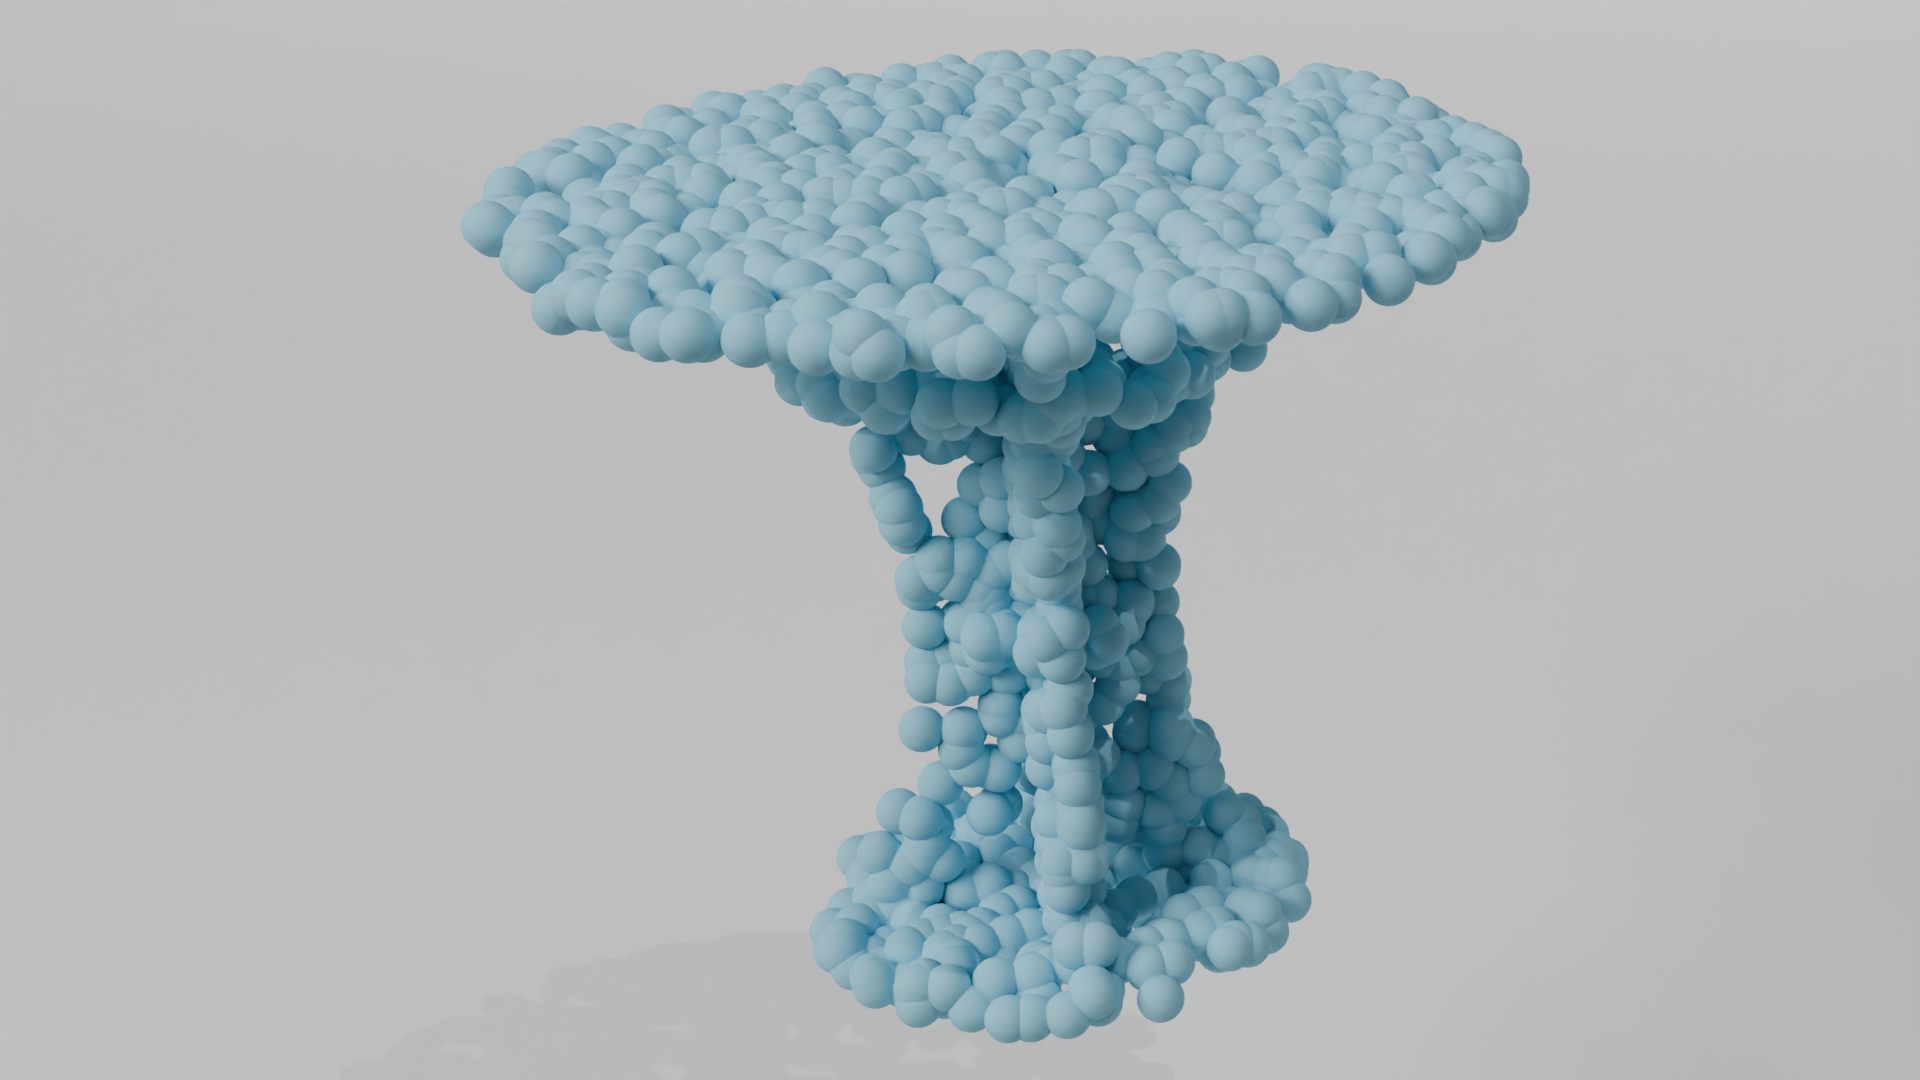
\includegraphics[width=\textwidth]{figures/com_t3.png}
        \caption{Table 3}
    \end{subfigure}
    \caption{Grid test}
    \label{fig:table}
\end{figure}